% Options for packages loaded elsewhere
\PassOptionsToPackage{unicode}{hyperref}
\PassOptionsToPackage{hyphens}{url}
\PassOptionsToPackage{dvipsnames,svgnames,x11names}{xcolor}
%
\documentclass[
  letterpaper,
  DIV=11,
  numbers=noendperiod]{scrreprt}

\usepackage{amsmath,amssymb}
\usepackage{iftex}
\ifPDFTeX
  \usepackage[T1]{fontenc}
  \usepackage[utf8]{inputenc}
  \usepackage{textcomp} % provide euro and other symbols
\else % if luatex or xetex
  \usepackage{unicode-math}
  \defaultfontfeatures{Scale=MatchLowercase}
  \defaultfontfeatures[\rmfamily]{Ligatures=TeX,Scale=1}
\fi
\usepackage{lmodern}
\ifPDFTeX\else  
    % xetex/luatex font selection
  \setmainfont[]{Lexend}
  \setmonofont[]{Fira Mono}
\fi
% Use upquote if available, for straight quotes in verbatim environments
\IfFileExists{upquote.sty}{\usepackage{upquote}}{}
\IfFileExists{microtype.sty}{% use microtype if available
  \usepackage[]{microtype}
  \UseMicrotypeSet[protrusion]{basicmath} % disable protrusion for tt fonts
}{}
\makeatletter
\@ifundefined{KOMAClassName}{% if non-KOMA class
  \IfFileExists{parskip.sty}{%
    \usepackage{parskip}
  }{% else
    \setlength{\parindent}{0pt}
    \setlength{\parskip}{6pt plus 2pt minus 1pt}}
}{% if KOMA class
  \KOMAoptions{parskip=half}}
\makeatother
\usepackage{xcolor}
\setlength{\emergencystretch}{3em} % prevent overfull lines
\setcounter{secnumdepth}{5}
% Make \paragraph and \subparagraph free-standing
\ifx\paragraph\undefined\else
  \let\oldparagraph\paragraph
  \renewcommand{\paragraph}[1]{\oldparagraph{#1}\mbox{}}
\fi
\ifx\subparagraph\undefined\else
  \let\oldsubparagraph\subparagraph
  \renewcommand{\subparagraph}[1]{\oldsubparagraph{#1}\mbox{}}
\fi

\usepackage{color}
\usepackage{fancyvrb}
\newcommand{\VerbBar}{|}
\newcommand{\VERB}{\Verb[commandchars=\\\{\}]}
\DefineVerbatimEnvironment{Highlighting}{Verbatim}{commandchars=\\\{\}}
% Add ',fontsize=\small' for more characters per line
\usepackage{framed}
\definecolor{shadecolor}{RGB}{241,243,245}
\newenvironment{Shaded}{\begin{snugshade}}{\end{snugshade}}
\newcommand{\AlertTok}[1]{\textcolor[rgb]{0.68,0.00,0.00}{#1}}
\newcommand{\AnnotationTok}[1]{\textcolor[rgb]{0.37,0.37,0.37}{#1}}
\newcommand{\AttributeTok}[1]{\textcolor[rgb]{0.40,0.45,0.13}{#1}}
\newcommand{\BaseNTok}[1]{\textcolor[rgb]{0.68,0.00,0.00}{#1}}
\newcommand{\BuiltInTok}[1]{\textcolor[rgb]{0.00,0.23,0.31}{#1}}
\newcommand{\CharTok}[1]{\textcolor[rgb]{0.13,0.47,0.30}{#1}}
\newcommand{\CommentTok}[1]{\textcolor[rgb]{0.37,0.37,0.37}{#1}}
\newcommand{\CommentVarTok}[1]{\textcolor[rgb]{0.37,0.37,0.37}{\textit{#1}}}
\newcommand{\ConstantTok}[1]{\textcolor[rgb]{0.56,0.35,0.01}{#1}}
\newcommand{\ControlFlowTok}[1]{\textcolor[rgb]{0.00,0.23,0.31}{#1}}
\newcommand{\DataTypeTok}[1]{\textcolor[rgb]{0.68,0.00,0.00}{#1}}
\newcommand{\DecValTok}[1]{\textcolor[rgb]{0.68,0.00,0.00}{#1}}
\newcommand{\DocumentationTok}[1]{\textcolor[rgb]{0.37,0.37,0.37}{\textit{#1}}}
\newcommand{\ErrorTok}[1]{\textcolor[rgb]{0.68,0.00,0.00}{#1}}
\newcommand{\ExtensionTok}[1]{\textcolor[rgb]{0.00,0.23,0.31}{#1}}
\newcommand{\FloatTok}[1]{\textcolor[rgb]{0.68,0.00,0.00}{#1}}
\newcommand{\FunctionTok}[1]{\textcolor[rgb]{0.28,0.35,0.67}{#1}}
\newcommand{\ImportTok}[1]{\textcolor[rgb]{0.00,0.46,0.62}{#1}}
\newcommand{\InformationTok}[1]{\textcolor[rgb]{0.37,0.37,0.37}{#1}}
\newcommand{\KeywordTok}[1]{\textcolor[rgb]{0.00,0.23,0.31}{#1}}
\newcommand{\NormalTok}[1]{\textcolor[rgb]{0.00,0.23,0.31}{#1}}
\newcommand{\OperatorTok}[1]{\textcolor[rgb]{0.37,0.37,0.37}{#1}}
\newcommand{\OtherTok}[1]{\textcolor[rgb]{0.00,0.23,0.31}{#1}}
\newcommand{\PreprocessorTok}[1]{\textcolor[rgb]{0.68,0.00,0.00}{#1}}
\newcommand{\RegionMarkerTok}[1]{\textcolor[rgb]{0.00,0.23,0.31}{#1}}
\newcommand{\SpecialCharTok}[1]{\textcolor[rgb]{0.37,0.37,0.37}{#1}}
\newcommand{\SpecialStringTok}[1]{\textcolor[rgb]{0.13,0.47,0.30}{#1}}
\newcommand{\StringTok}[1]{\textcolor[rgb]{0.13,0.47,0.30}{#1}}
\newcommand{\VariableTok}[1]{\textcolor[rgb]{0.07,0.07,0.07}{#1}}
\newcommand{\VerbatimStringTok}[1]{\textcolor[rgb]{0.13,0.47,0.30}{#1}}
\newcommand{\WarningTok}[1]{\textcolor[rgb]{0.37,0.37,0.37}{\textit{#1}}}

\providecommand{\tightlist}{%
  \setlength{\itemsep}{0pt}\setlength{\parskip}{0pt}}\usepackage{longtable,booktabs,array}
\usepackage{calc} % for calculating minipage widths
% Correct order of tables after \paragraph or \subparagraph
\usepackage{etoolbox}
\makeatletter
\patchcmd\longtable{\par}{\if@noskipsec\mbox{}\fi\par}{}{}
\makeatother
% Allow footnotes in longtable head/foot
\IfFileExists{footnotehyper.sty}{\usepackage{footnotehyper}}{\usepackage{footnote}}
\makesavenoteenv{longtable}
\usepackage{graphicx}
\makeatletter
\def\maxwidth{\ifdim\Gin@nat@width>\linewidth\linewidth\else\Gin@nat@width\fi}
\def\maxheight{\ifdim\Gin@nat@height>\textheight\textheight\else\Gin@nat@height\fi}
\makeatother
% Scale images if necessary, so that they will not overflow the page
% margins by default, and it is still possible to overwrite the defaults
% using explicit options in \includegraphics[width, height, ...]{}
\setkeys{Gin}{width=\maxwidth,height=\maxheight,keepaspectratio}
% Set default figure placement to htbp
\makeatletter
\def\fps@figure{htbp}
\makeatother

\KOMAoption{captions}{tableheading}
\makeatletter
\makeatother
\makeatletter
\makeatother
\makeatletter
\@ifpackageloaded{caption}{}{\usepackage{caption}}
\AtBeginDocument{%
\ifdefined\contentsname
  \renewcommand*\contentsname{Table of contents}
\else
  \newcommand\contentsname{Table of contents}
\fi
\ifdefined\listfigurename
  \renewcommand*\listfigurename{List of Figures}
\else
  \newcommand\listfigurename{List of Figures}
\fi
\ifdefined\listtablename
  \renewcommand*\listtablename{List of Tables}
\else
  \newcommand\listtablename{List of Tables}
\fi
\ifdefined\figurename
  \renewcommand*\figurename{Figure}
\else
  \newcommand\figurename{Figure}
\fi
\ifdefined\tablename
  \renewcommand*\tablename{Table}
\else
  \newcommand\tablename{Table}
\fi
}
\@ifpackageloaded{float}{}{\usepackage{float}}
\floatstyle{ruled}
\@ifundefined{c@chapter}{\newfloat{codelisting}{h}{lop}}{\newfloat{codelisting}{h}{lop}[chapter]}
\floatname{codelisting}{Listing}
\newcommand*\listoflistings{\listof{codelisting}{List of Listings}}
\makeatother
\makeatletter
\@ifpackageloaded{caption}{}{\usepackage{caption}}
\@ifpackageloaded{subcaption}{}{\usepackage{subcaption}}
\makeatother
\makeatletter
\@ifpackageloaded{tcolorbox}{}{\usepackage[skins,breakable]{tcolorbox}}
\makeatother
\makeatletter
\@ifundefined{shadecolor}{\definecolor{shadecolor}{rgb}{.97, .97, .97}}
\makeatother
\makeatletter
\makeatother
\makeatletter
\makeatother
\ifLuaTeX
  \usepackage{selnolig}  % disable illegal ligatures
\fi
\IfFileExists{bookmark.sty}{\usepackage{bookmark}}{\usepackage{hyperref}}
\IfFileExists{xurl.sty}{\usepackage{xurl}}{} % add URL line breaks if available
\urlstyle{same} % disable monospaced font for URLs
\hypersetup{
  pdftitle={Intro to Linux},
  pdfauthor={Matthew R. Gemmell},
  colorlinks=true,
  linkcolor={blue},
  filecolor={Maroon},
  citecolor={Blue},
  urlcolor={Blue},
  pdfcreator={LaTeX via pandoc}}

\title{Intro to Linux}
\author{Matthew R. Gemmell}
\date{2023-11-29}

\begin{document}
\maketitle
\ifdefined\Shaded\renewenvironment{Shaded}{\begin{tcolorbox}[breakable, enhanced, boxrule=0pt, frame hidden, borderline west={3pt}{0pt}{shadecolor}, interior hidden, sharp corners]}{\end{tcolorbox}}\fi

\renewcommand*\contentsname{Table of contents}
{
\hypersetup{linkcolor=}
\setcounter{tocdepth}{2}
\tableofcontents
}
\hypertarget{intro}{%
\chapter{Introduction}\label{intro}}

\begin{figure}

{\centering 
\includegraphics[width=0.3\textwidth,height=\textheight]{figures/NEOF.png}

}

\end{figure}

\begin{figure}

{\centering 
\includegraphics[width=0.2\textwidth,height=\textheight]{figures/linux_beginner.png}

}

\end{figure}

Bioinformatics is an increasingly important skill for biological
scientists. Many bioinformatic tools can only be run on Linux based
operating systems. This course aims to introduce you to Linux and is
aimed at beginners and novices to the command line.

Sessions will start with a brief presentation followed by self-paced
computer practicals guided by an online interactive book. The book will
contain theory, practice code, and exercises. Multiple choice questions
will help reinforce what you have learnt throughout the book.

At the end of the course learners will be able to:

\begin{itemize}
\tightlist
\item
  Explain how the user, shell, and kernel interact with each other in
  the Linux OS.
\item
  Navigate \& manipulate directories in the Linux environment.
\item
  List and view the contents of directories.
\item
  Carry out a variety of commands with files including printing them to
  terminal.
\item
  Utilise the text editor nano to create, edit, and save files.
\item
  Understand the structure of fastq files.
\end{itemize}

There are additional materials in chapters 12-14 which include some
advanced Linux commands and introductions to other programming languages
used by bioinformaticians.

Commands are in the following font, colour, and box. They should be run
in the command line.

\begin{Shaded}
\begin{Highlighting}[]
\BuiltInTok{echo} \StringTok{"This is a command example"} 
\end{Highlighting}
\end{Shaded}

In some chapters there are video walk-throughs. These are optional and
give you a guided visual walk-through of running the practice code in
the chapter. These are found in an expandable box at the start of the
chapters 4,5,6, and 8.

Additionally, please use the \protect\hyperlink{cheatsheet}{cheatsheet}
as a reminder of all the commands you will be learning.

\hypertarget{table-of-contents}{%
\section*{Table of contents}\label{table-of-contents}}
\addcontentsline{toc}{section}{Table of contents}

\markright{Table of contents}

\begin{longtable}[]{@{}
  >{\centering\arraybackslash}p{(\columnwidth - 2\tabcolsep) * \real{0.5109}}
  >{\centering\arraybackslash}p{(\columnwidth - 2\tabcolsep) * \real{0.4891}}@{}}
\toprule\noalign{}
\endhead
\bottomrule\noalign{}
\endlastfoot
\begin{minipage}[t]{\linewidth}\centering
\protect\hyperlink{linuxintro}{\textbf{What is Linux?}}

\begin{figure}

{\centering 

\protect\hyperlink{linuxintro}{
\includegraphics[width=1.47917in,height=\textheight]{figures/linux_beginner.png}}

}

\end{figure}
\end{minipage} & \begin{minipage}[t]{\linewidth}\centering
\protect\hyperlink{cluster}{\textbf{Logging in to our teaching VNC}}

\begin{figure}

{\centering 

\protect\hyperlink{cluster}{
\includegraphics[width=1.96875in,height=\textheight]{figures/start.png}}

}

\end{figure}
\end{minipage} \\
\begin{minipage}[t]{\linewidth}\centering
\protect\hyperlink{dirsandfiles}{\textbf{Directories and files}}

\begin{figure}

{\centering 

\protect\hyperlink{dirsandfiles}{
\includegraphics[width=1.30208in,height=\textheight]{figures/directory.png}}

}

\end{figure}
\end{minipage} & \begin{minipage}[t]{\linewidth}\centering
\protect\hyperlink{tipsandtricks}{\textbf{Tips and tricks}}

\begin{figure}

{\centering 

\protect\hyperlink{tipsandtricks}{
\includegraphics[width=3.14583in,height=\textheight]{figures/skateboard_trick.png}}

}

\end{figure}
\end{minipage} \\
\begin{minipage}[t]{\linewidth}\centering
\protect\hyperlink{manipulatingdirectories}{\textbf{Manipulating
Directories}}

\begin{figure}

{\centering 

\protect\hyperlink{manipulatingdirectories}{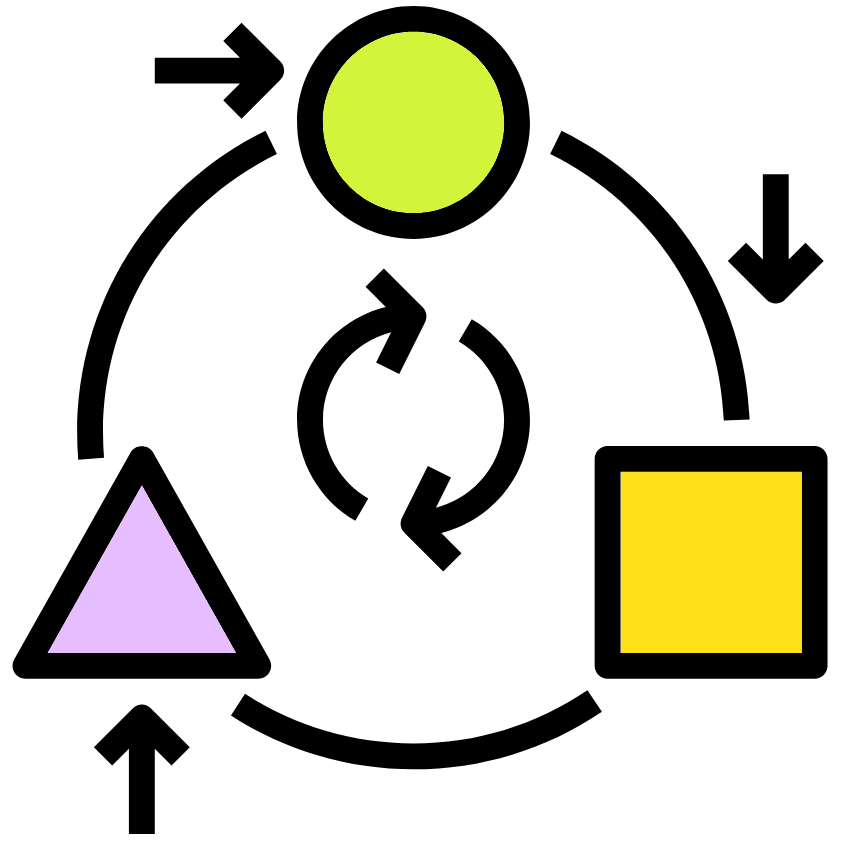
\includegraphics[width=1.5625in,height=\textheight]{figures/transform.png}}

}

\end{figure}
\end{minipage} & \begin{minipage}[t]{\linewidth}\centering
\protect\hyperlink{filereadingandprocessing}{\textbf{File reading and
processing}}

\begin{figure}

{\centering 

\protect\hyperlink{filereadingandprocessing}{
\includegraphics[width=2.13542in,height=\textheight]{figures/files.png}}

}

\end{figure}
\end{minipage} \\
\begin{minipage}[t]{\linewidth}\centering
\protect\hyperlink{advancedlinux}{\textbf{Advanced Linux}}

\begin{figure}

{\centering 

\protect\hyperlink{advancedlinux}{
\includegraphics[width=1.47917in,height=\textheight]{figures/linux_intermdiary.png}}

}

\end{figure}
\end{minipage} & \begin{minipage}[t]{\linewidth}\centering
\protect\hyperlink{bfxlanguages}{\textbf{Other Bioinformatics
programming languages}}

\begin{figure}

{\centering 

\protect\hyperlink{bfxlanguages}{
\includegraphics[width=1.65625in,height=\textheight]{figures/languages.png}}

}

\end{figure}
\end{minipage} \\
\begin{minipage}[t]{\linewidth}\centering
\protect\hyperlink{cheatsheet}{\textbf{Appendix}}

\begin{figure}

{\centering 

\protect\hyperlink{cheatsheet}{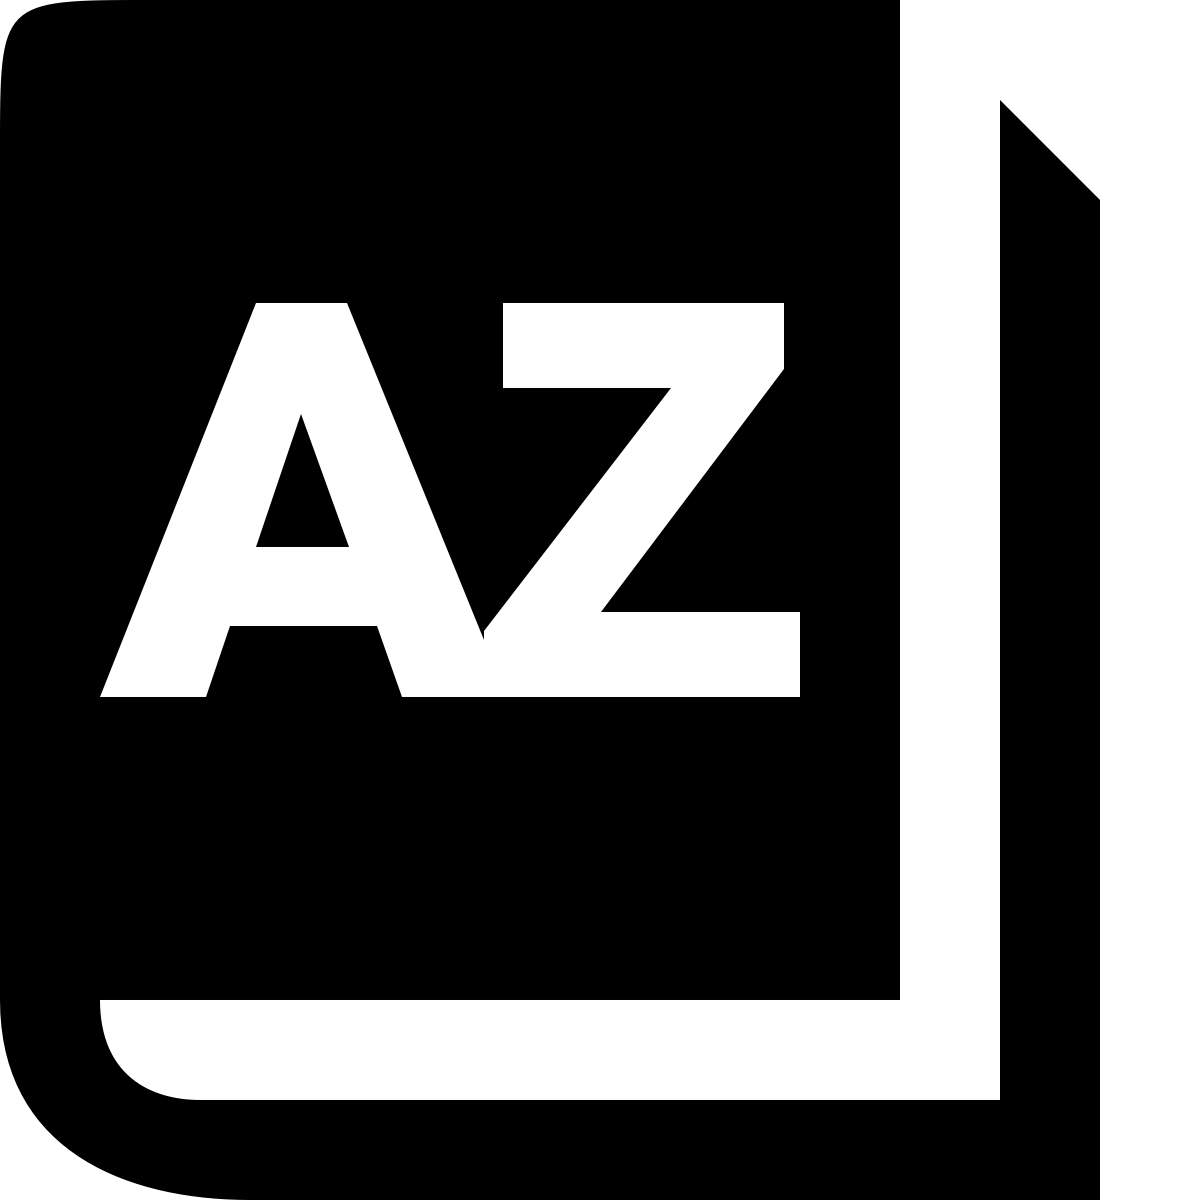
\includegraphics[width=1.5625in,height=\textheight]{figures/cheatsheet.png}}

}

\end{figure}
\end{minipage} & \\
\end{longtable}

This work is licensed under a Creative Commons
Attribution-NonCommercial-ShareAlike 4.0 International License.

\part{Start}

\part{Part 1}

\hypertarget{linuxintro}{%
\chapter{Linux}\label{linuxintro}}

\begin{figure}

{\centering 
\includegraphics[width=0.2\textwidth,height=\textheight]{figures/linux_beginner.png}

}

\end{figure}

Linux is a multitasking, multiuser Unix-like computer operating system
(OS). Linux can run many different applications (multitasking) and it
can be used by many different people (multiuser) on the same computer at
the same time.

It is utilised by many programmers, including Bioinformaticians. It is a
relatively easy OS to run commands and develop software for. The vast
majority of programs and tools for computational analysis of biological
data will work in Linux.

There are three parts of the Linux OS:

\begin{itemize}
\tightlist
\item
  \textbf{The kernel}: This is the hub of the operating systems. This is
  the ``behind the scenes'' part of the OS which allocates time and
  memory to programs. This controls the hardware.
\item
  \textbf{The shell}: This acts as the interface between the user and
  the kernel. When a user runs commands, the shell will interpret these
  commands for the kernel. The shell can be any program that constitutes
  the user interface e.g.~command line, internet browser, start menu
  etc.
\item
  \textbf{Programs}: Programs allow the OS to perform specific tasks.
  Examples of programs include Internet browsers, genome assembly tools,
  text editors etc.
\end{itemize}

\begin{figure}

{\centering 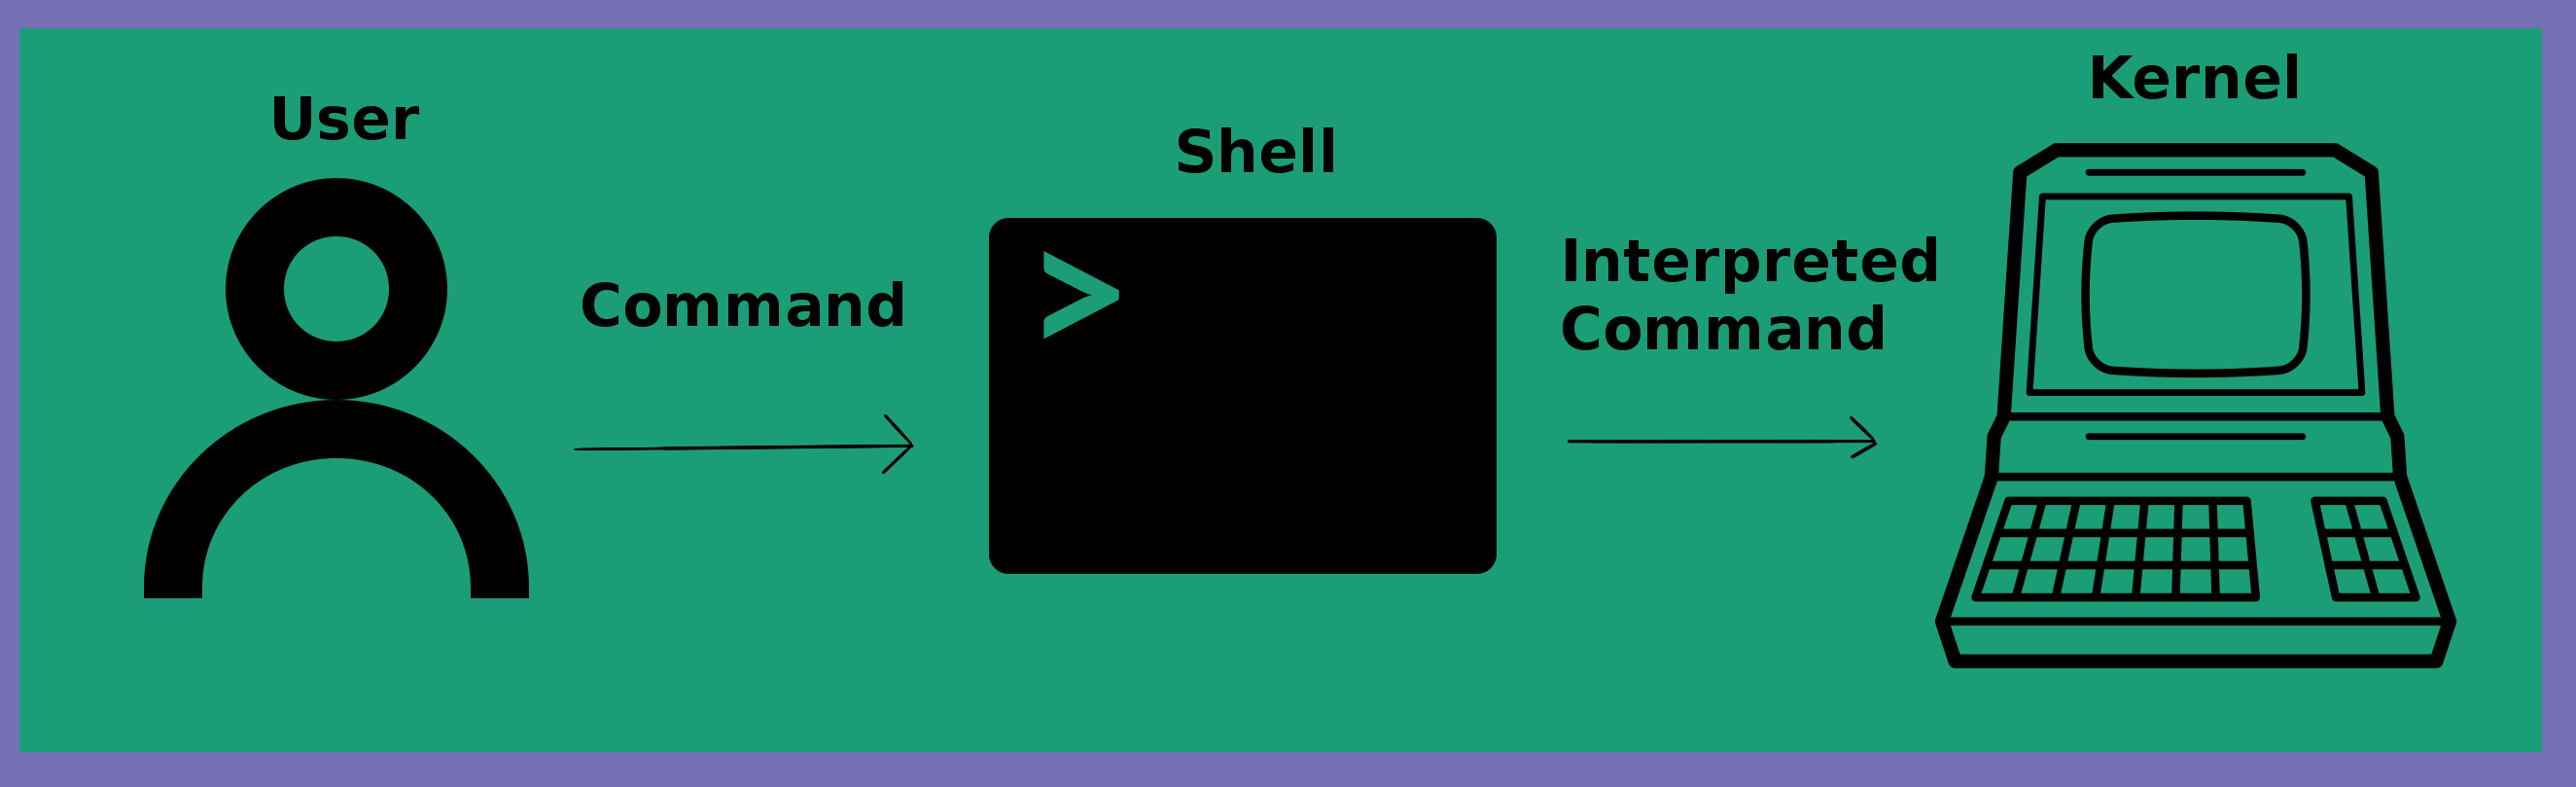
\includegraphics[width=0.8\textwidth,height=\textheight]{figures/linux_user_to_kernel.png}

}

\end{figure}

It is important to learn the Linux language so you can run commands on
the command line. This is because:

\begin{itemize}
\tightlist
\item
  Many bioinformatic tools do not have a graphical user interface (gui)
  and so must be run on the command line.
\item
  There are many powerful commands that can be run on the Linux command
  line.
\item
  It is quicker and more reproducible to run commands through a shell
  than through a gui.
\end{itemize}

\hypertarget{starting}{%
\chapter{Starting}\label{starting}}

\begin{figure}

{\centering 
\includegraphics[width=0.2\textwidth,height=\textheight]{figures/start.png}

}

\end{figure}

\hypertarget{cluster}{%
\section{Logon instructions}\label{cluster}}

For this workshop we will be using Virtual Network Computing (VNC).
Connect to the VNC with a browser by using the webVNC link you were
sent.

You will now be in a logged-in Linux VNC desktop with two terminals. You
will see something as below (there may be only one terminal which is
fine). If you do not see something similar please ask for assistance.

\begin{figure}

{\centering 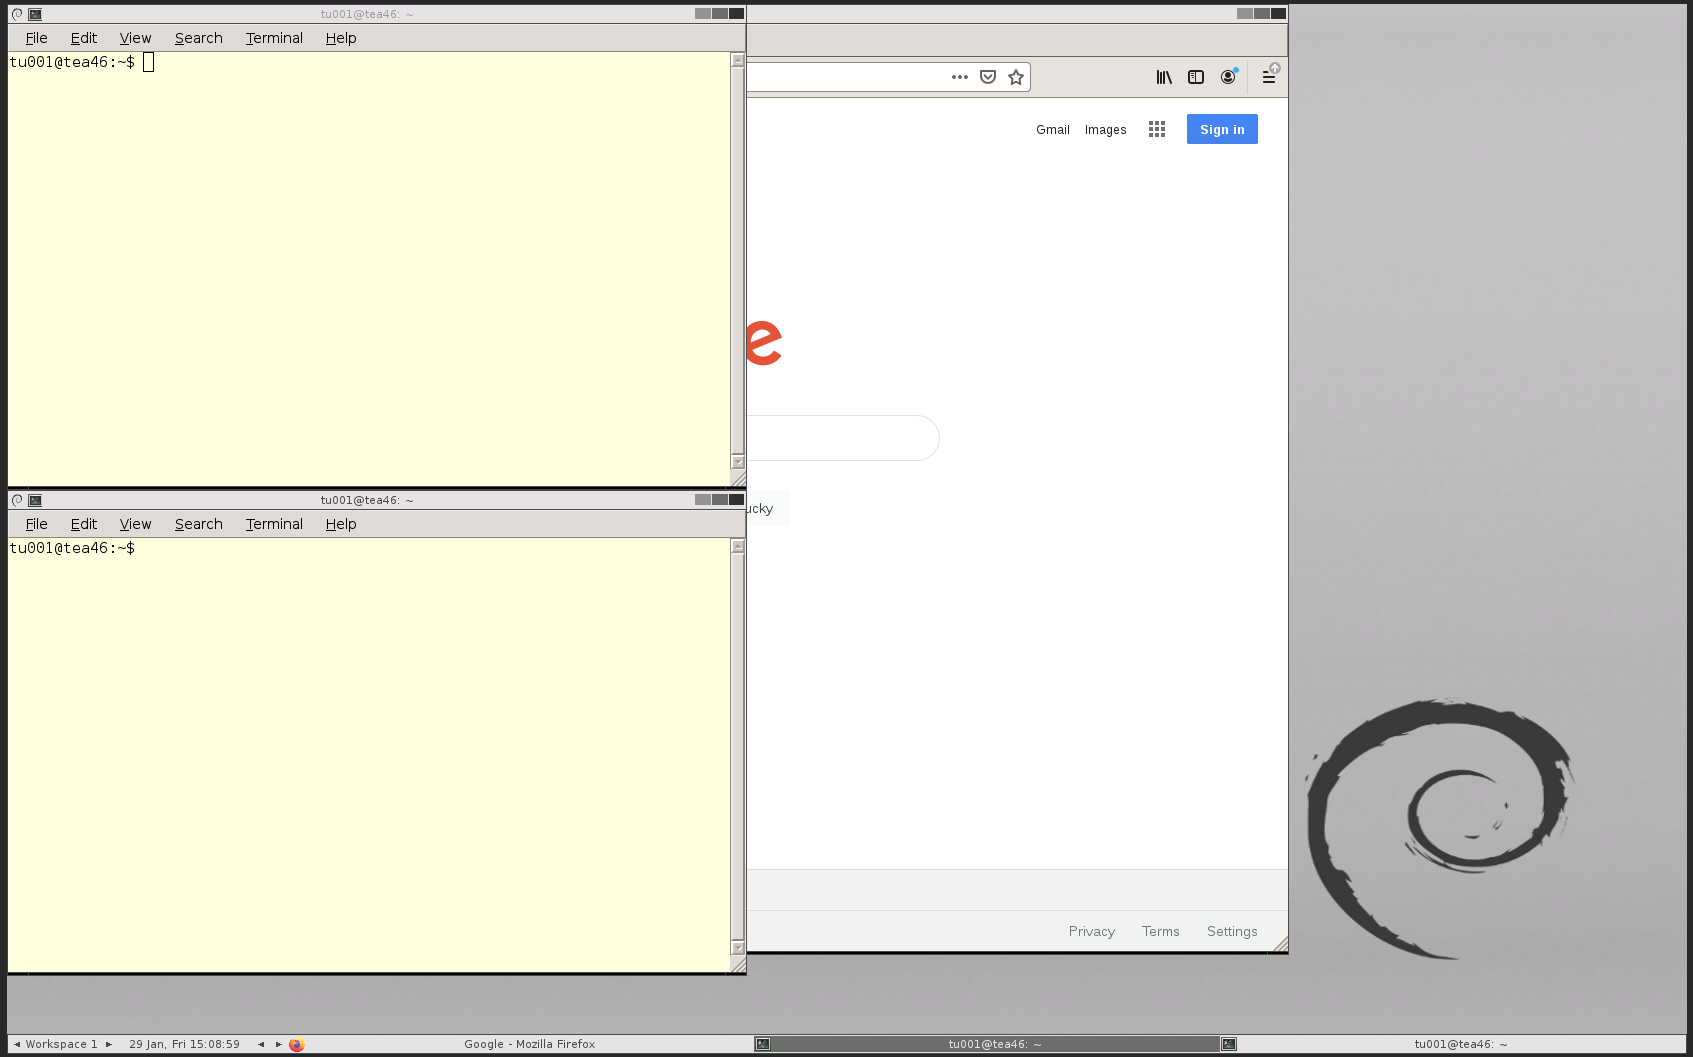
\includegraphics[width=0.8\textwidth,height=\textheight]{figures/logon_pic.png}

}

\end{figure}

If the VNC is taking up too much/little space of your browser you can
use the zoom of your browser to adjust the size. Ensure you can see one
whole terminal.

These instructions will not work outside of this workshop. If you would
like to install your own Linux OS on your desktop or laptop we would
recommend Mint Linux

The following link is a guide to install Mint Linux:\\
https://linuxmint-installation-guide.readthedocs.io/en/latest/

\hypertarget{the-terminal-window}{%
\section{The Terminal Window}\label{the-terminal-window}}

In our case the terminal window looks like the picture below. We are
using the terminal window as our shell to interpret our commands to the
kernel. Depending on your system and preferences it may look different.

\begin{figure}

{\centering 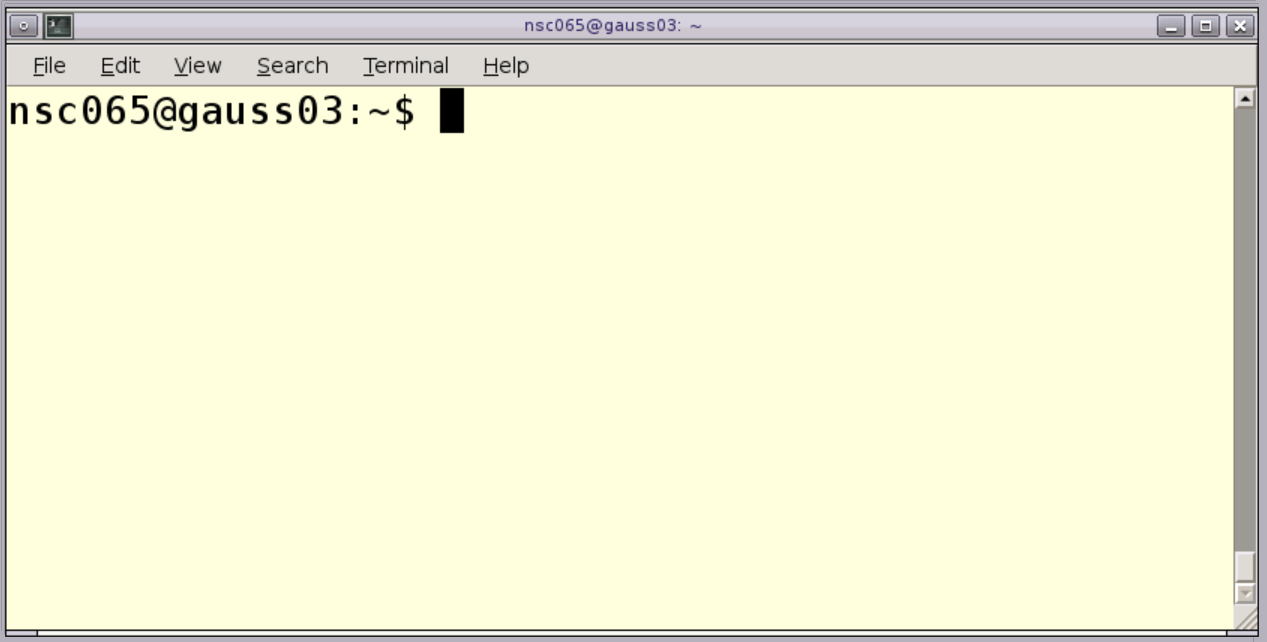
\includegraphics[width=0.8\textwidth,height=\textheight]{figures/terminal_window.png}

}

\end{figure}

Already there is useful information for us on the terminal window.

\begin{itemize}
\tightlist
\item
  \textbf{nsc006}: This is the login name, also known as the username.
  In this case nsc006 is a demonstrator's account. Your screen should
  show a different account name which will be your username for the
  Linux machine/cluster you are logged into.
\item
  \textbf{gauss03}: This is the machine name the user is logged into.
\item
  \textbf{\textasciitilde{}}: This represents the current directory of
  the user, or the directory a command was run in. In the Linux OS and
  others \textbf{`\textasciitilde{}'} is a shortcut to the user's home
  directory.
\item
  Everything after the \textbf{`\$'} is where commands are typed into
  the terminal. This is also referred to as the command line.
\end{itemize}

To open a new terminal window, right click on the main screen, choose
\texttt{Applications} -\textgreater{} \texttt{Shell} -\textgreater{}
\texttt{bash}

\hypertarget{commands}{%
\section{Commands}\label{commands}}

Commands are typed into the terminal and then run by pressing
\textbf{``enter''}''

\begin{figure}

{\centering 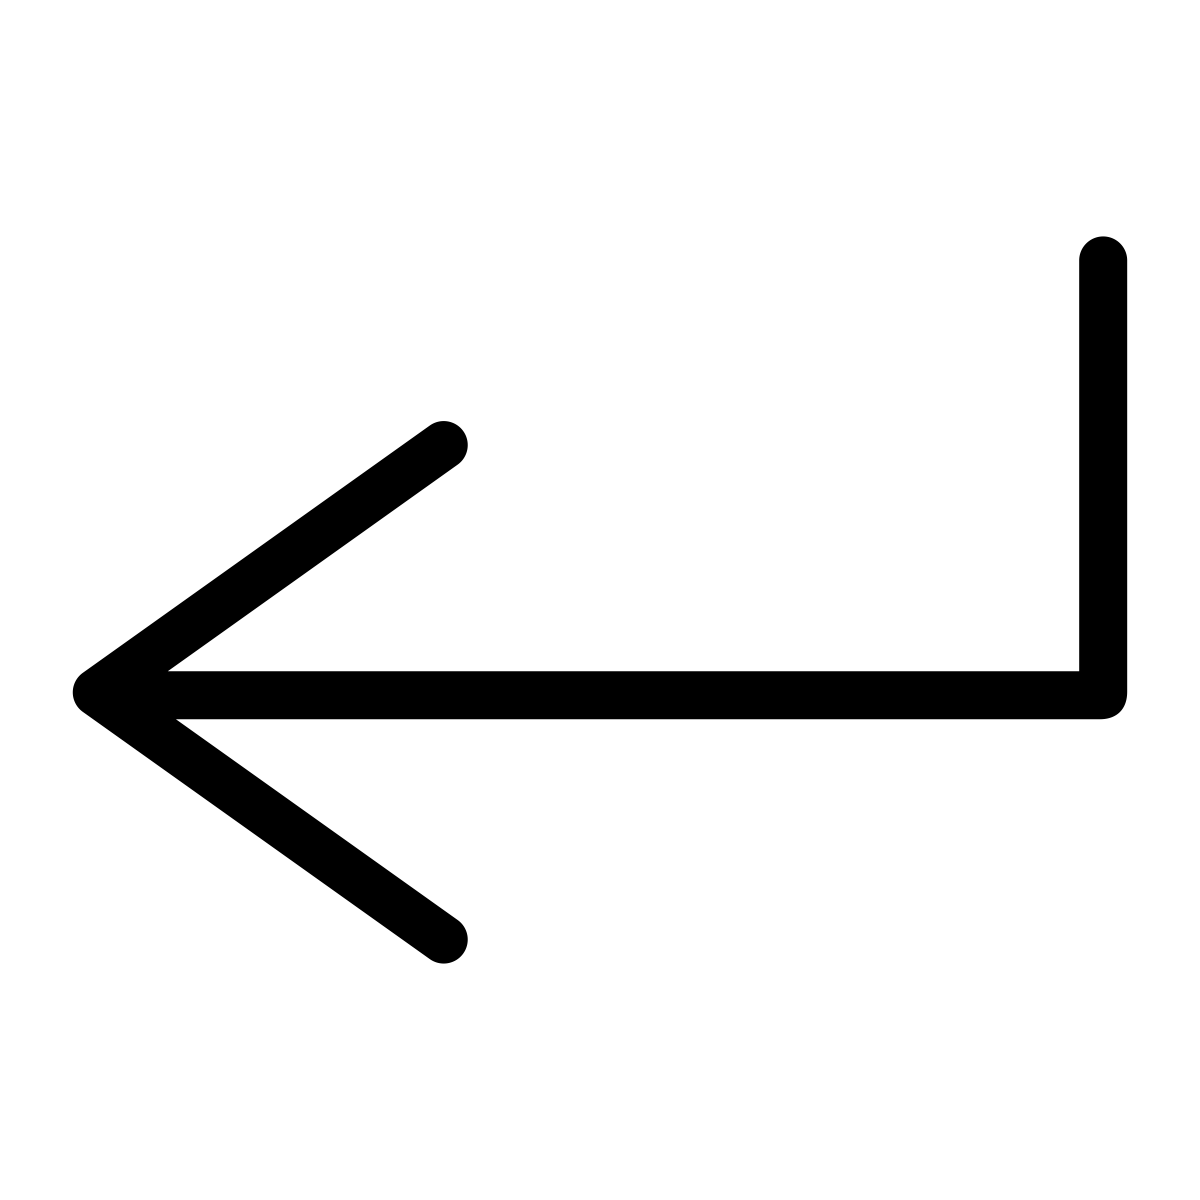
\includegraphics[width=0.2\textwidth,height=\textheight]{figures/enter_symbol.png}

}

\end{figure}

To run a command select your terminal by clicking on it or using
\textbf{``alt+shift''}.

Now run the below command:

\begin{Shaded}
\begin{Highlighting}[]
\BuiltInTok{echo} \StringTok{"Hello World"}
\end{Highlighting}
\end{Shaded}

In this case \texttt{echo} is a command that prints out the term ``Hello
World''.

Now try:

\begin{Shaded}
\begin{Highlighting}[]
\BuiltInTok{echo} \StringTok{"Bye World"}
\end{Highlighting}
\end{Shaded}

There are many different Linux commands and we will run through a few.
With a large variety it can be hard to remember all the commands and how
they work.

Three convenient resources are:

\begin{enumerate}
\def\labelenumi{\arabic{enumi}.}
\tightlist
\item
  \textbf{Search engines} (e.g.~Google): There are many forums where
  people ask for help with command line issues. If you have an issue and
  are not sure what to do, most likely someone else has had the same
  issue and asked for help on a forum. The tricky part of this is
  knowing the specific terminology to use when searching. Forums where
  people ask bioinformatics questions include SEQanswers, Stack overflow
  and biostars.
\item
  \textbf{Cheat sheets}: It is never wrong to ``cheat'' when coding.
  Cheat sheets with many commands and good descriptions are very useful.
  Here is a good example of one:
  \url{https://files.fosswire.com/2007/08/fwunixref.pdf}
\item
  \textbf{Manual pages}: Linux commands have many different parameters
  and options. If you ever need to figure out what they all are and what
  they do you can use the \texttt{man} command.
\end{enumerate}

E.g. The below command will show the manual page for the echo command:

\begin{Shaded}
\begin{Highlighting}[]
\FunctionTok{man}\NormalTok{ echo}
\end{Highlighting}
\end{Shaded}

The below command will show the manual page for the \texttt{man}
command:

\begin{Shaded}
\begin{Highlighting}[]
\FunctionTok{man}\NormalTok{ man}
\end{Highlighting}
\end{Shaded}

\textbf{Note}: The \texttt{man} page acts like using the command
\textbf{less} (we will get into more specifics later). Important notes
for now are to use the \textbf{arrow keys} to go \textbf{up} and
\textbf{down} the page and press \textbf{q} to exit the manual

\textbf{Note}: There is a cheat sheet at the end of this document with
all the commands covered in this practical.

\hypertarget{dirsandfiles}{%
\chapter{Directories and Files}\label{dirsandfiles}}

\begin{figure}

{\centering 
\includegraphics[width=0.2\textwidth,height=\textheight]{figures/directory.png}

}

\end{figure}

Chapter 4 video walk-through

\hypertarget{acquiring-workshop-data}{%
\section{Acquiring Workshop data}\label{acquiring-workshop-data}}

The first step to carry out is to copy the data for the workshop to your
home directory.

\hypertarget{changing-directories}{%
\subsection{Changing directories}\label{changing-directories}}

Before copying you will change directory to your home directory.

\begin{itemize}
\tightlist
\item
  \texttt{cd} is the command to Change Directory. It is followed by the
  directory you want to change to.
\item
  \textbf{``\textasciitilde{}''} represents your home directory.
\end{itemize}

Change directory to your home directory by running the following command
in your terminal:

\begin{Shaded}
\begin{Highlighting}[]
\BuiltInTok{cd}\NormalTok{ \textasciitilde{} }
\end{Highlighting}
\end{Shaded}

In Linux the default of \texttt{cd} is to change directory to your home
directory. Therefore the following command will do the same as the
above.

\begin{Shaded}
\begin{Highlighting}[]
\BuiltInTok{cd}
\end{Highlighting}
\end{Shaded}

To determine your current working directory you can either look at the
part of the terminal which displays it or you can use the command
\texttt{pwd} (print working directory). Enter the following command:

\begin{Shaded}
\begin{Highlighting}[]
\BuiltInTok{pwd}
\end{Highlighting}
\end{Shaded}

In this case it will not show a \textbf{``\textasciitilde{}''} but the
full path of your home directory. E.g. \textbf{``/pub14/tea/nsc206/''}.

\begin{itemize}
\tightlist
\item
  The first \textbf{``/''} is the root of the system. Every directory,
  subdirectory, file and program of the machine is within the root.
\item
  \textbf{``pub14/''}: A directory within the root.
\item
  \textbf{``tea/''}: A subdirectory of \textbf{``pub14/''} and a
  sub-subdirectory of the root (\textbf{``/''}).
\item
  \textbf{``nsc206''}: The home directory of user nsc206. It is a
  subdirectory of \textbf{``tea/''} which is a subdirectory of
  \textbf{``pub14/''} which is a subdirectory of the root
  (\textbf{``/''}).
\end{itemize}

\hypertarget{copying}{%
\subsection{Copying}\label{copying}}

Now that we are in our home directory we can copy the data we need to
it.

To do this we can use the command \texttt{cp}. This command is followed
by the directory/file we want to copy then by the directory we want to
copy it to.

To copy a directory we need to add the option \texttt{-r} which means
recursively copy this directory and all its contents. Otherwise
\texttt{cp} can only be used to copy files.

Use the below command to copy the workshop data to your current
directory. The \textbf{``.''} refers to your current directory.

\begin{Shaded}
\begin{Highlighting}[]
\FunctionTok{cp} \AttributeTok{{-}r}\NormalTok{ /pub14/tea/nsc206/NEOF/Linux/ .}
\end{Highlighting}
\end{Shaded}

Now change directory into your newly copied directory.

\begin{Shaded}
\begin{Highlighting}[]
\BuiltInTok{cd}\NormalTok{ Linux}
\end{Highlighting}
\end{Shaded}

Print to screen the path of your current working directory.

\begin{Shaded}
\begin{Highlighting}[]
\BuiltInTok{pwd}
\end{Highlighting}
\end{Shaded}

\hypertarget{directory-structure}{%
\section{Directory structure}\label{directory-structure}}

You can think of the directory structure in two different ways.

\hypertarget{the-directory-tree}{%
\subsection{The Directory tree}\label{the-directory-tree}}

This starts as the root (\textbf{``/''}) which branches out into
directories and files. Directories contain files and subdirectories
which contain files and subdirectories etc.

Below is an example of visualising the location of the
\textbf{``Linux''} directory within the user ncs006's home directory as
a tree. This only includes a subset of directories.

\begin{figure}

{\centering 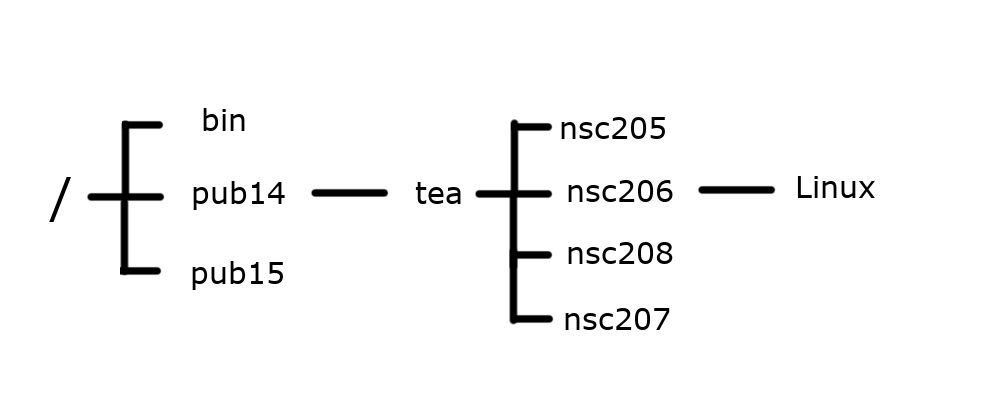
\includegraphics[width=1\textwidth,height=\textheight]{figures/linux_tree_structure.png}

}

\end{figure}

\hypertarget{boxes}{%
\subsection{Boxes}\label{boxes}}

Another analogy to the directory structure is boxes and items. In this
case there is one large box that contains all the boxes and items, this
is the root (\textbf{``/''}). In the root are items and boxes which hold
items and boxes etc.

Below is an example of visualising the location of the
\textbf{``Linux''} directory within the user ncs006's home directory as
boxes. This only includes a subset of directories.

\begin{figure}

{\centering 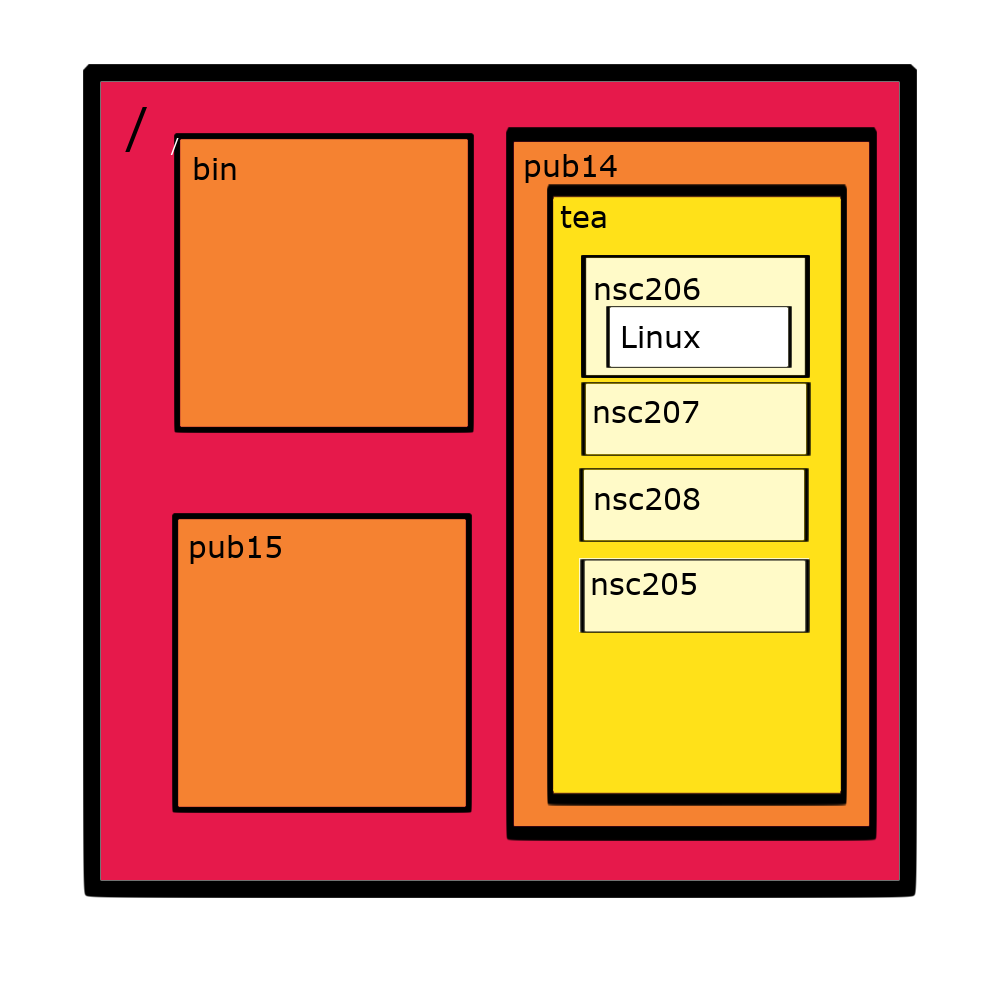
\includegraphics[width=0.6\textwidth,height=\textheight]{figures/linux_box_structure.png}

}

\end{figure}

\hypertarget{paths}{%
\section{Paths}\label{paths}}

\begin{figure}

{\centering 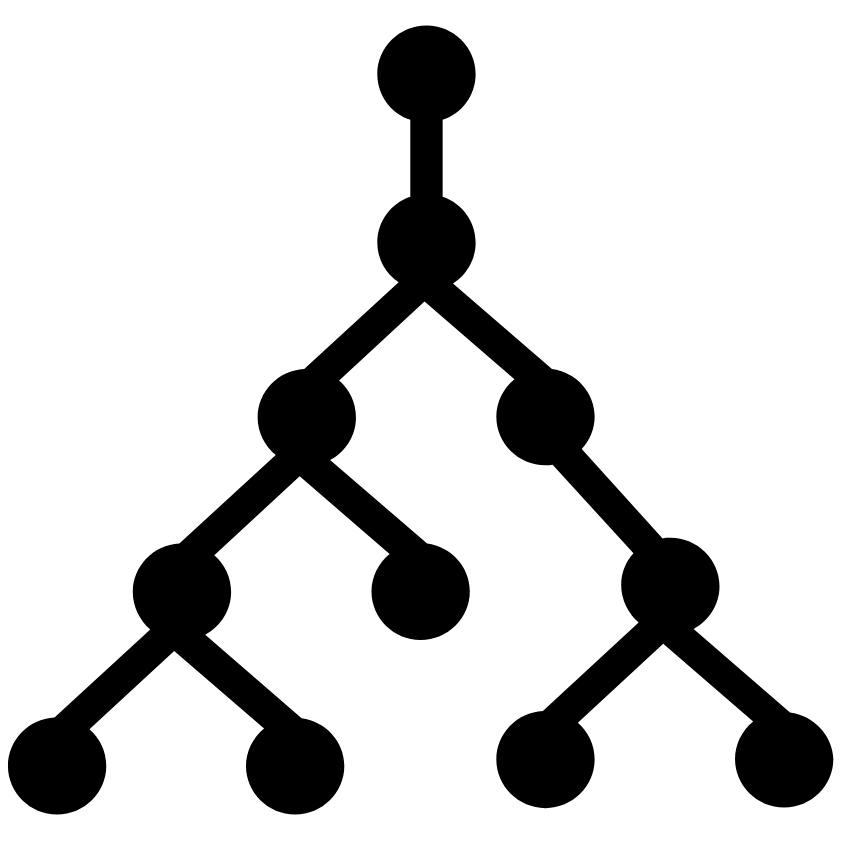
\includegraphics[width=0.2\textwidth,height=\textheight]{figures/paths.png}

}

\end{figure}

On the command line directories and files are referred to by paths
e.g.~\textbf{``/pub14/tea/nsc206/Linux/''} is a path.

Paths are case sensitive. The path \textbf{``directory/file.txt''} is
different than \textbf{``diRectory/File.txt''}.

Spaces should always be avoided in path names. It is highly recommended
to \textbf{``\_''} instead. This is because spaces are used to separate
options and parameters in commands.

There are multiple ways to refer to a path. The two main ways are
through \textbf{absolute paths} and \textbf{relative paths}.

\hypertarget{absolute-paths}{%
\subsection{Absolute paths}\label{absolute-paths}}

Absolute paths are paths that start from the root e.g.

\begin{itemize}
\tightlist
\item
  \textbf{``/pub14/tea/nsc206/Linux/''}
\item
  \textbf{``\textasciitilde/Linux/''} (In this case \textasciitilde{} is
  a shortcut which includes the root)
\item
  \textbf{``/pub14/tea/nsc206/file.txt''}
\end{itemize}

\hypertarget{relative-paths}{%
\subsection{Relative paths}\label{relative-paths}}

Relative paths are paths that are relative to another location besides
the root e.g.

\begin{itemize}
\tightlist
\item
  \textbf{``.''} (This means the current working directory).
\item
  \textbf{``..''} (This refers to one directory up e.g.~if the current
  directory was \textbf{``/pub14/tea/nsc206/''}, the \textbf{``..''}
  directory would be \textbf{``/pub14/tea/''}).
\item
  \textbf{``1\_directory/''}, would refer to the directory
  \textbf{``1\_directory/''} in your current directory
\end{itemize}

\hypertarget{change-directory-examples}{%
\subsection{Change directory examples}\label{change-directory-examples}}

Below is a subset of valid methods to change directory into your
\textbf{``Linux/''} directory

\textbf{Note}:change \textbf{nsc2xx} to your specific user name as shown
on the command line prompt.

Method 1

\begin{Shaded}
\begin{Highlighting}[]
\BuiltInTok{cd}\NormalTok{ /pub14/tea/nsc2xx/Linux/}
\end{Highlighting}
\end{Shaded}

Method 2

\begin{Shaded}
\begin{Highlighting}[]
\BuiltInTok{cd}\NormalTok{ \textasciitilde{}}
\BuiltInTok{cd}\NormalTok{ Linux/}
\end{Highlighting}
\end{Shaded}

Method 3

\begin{Shaded}
\begin{Highlighting}[]
\BuiltInTok{cd}\NormalTok{ /pub14/tea/nsc2xx/Linux/1\_directory/}
\BuiltInTok{cd}\NormalTok{ ..}
\end{Highlighting}
\end{Shaded}

Method 4

\begin{Shaded}
\begin{Highlighting}[]
\BuiltInTok{cd}\NormalTok{ /pub14/}
\BuiltInTok{cd}\NormalTok{ tea/}
\BuiltInTok{cd}\NormalTok{ nsc2xx/}
\BuiltInTok{cd}\NormalTok{ Linux/}
\end{Highlighting}
\end{Shaded}

\hypertarget{listing-directory-content}{%
\section{Listing Directory content}\label{listing-directory-content}}

\begin{figure}

{\centering 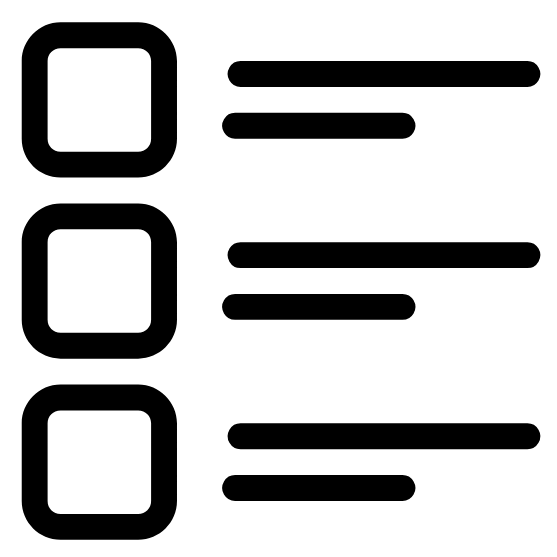
\includegraphics[width=0.2\textwidth,height=\textheight]{figures/List.png}

}

\end{figure}

To list the contents (files and directories) within a directory you can
use the \texttt{ls} command.

The output of \texttt{ls} will include file names that are coloured
black and directory names that are coloured blue in our VNC terminals.

Before carrying out the below commands make sure you are in your
\textbf{``Linux''} directory with the \texttt{pwd} command.

List the contents in your current directory:

\begin{Shaded}
\begin{Highlighting}[]
\FunctionTok{ls}
\end{Highlighting}
\end{Shaded}

List the contents in your home directory:

\begin{Shaded}
\begin{Highlighting}[]
\FunctionTok{ls}\NormalTok{ ..}
\end{Highlighting}
\end{Shaded}

List the contents in the root directory and put each separate
file/directory on a separate line. In the below command the \texttt{-1}
is a parameter that indicates there will be only 1 piece of content on
each line. Note: \texttt{-2}, \texttt{-3} etc are not parameters that
work with \texttt{ls}.

\begin{Shaded}
\begin{Highlighting}[]
\FunctionTok{ls} \AttributeTok{{-}1}\NormalTok{ /}
\end{Highlighting}
\end{Shaded}

\textbf{Reminder}: you can use the \texttt{man} command to look at more
options for commands.

\texttt{ls} is my most typed command. I am consistently using it to see
what directories and files are in my current directory and other
directories. I suggest you do the same.

\hypertarget{mcqs-files-directories}{%
\section{MCQs: Files \& Directories}\label{mcqs-files-directories}}

\begin{figure}

{\centering 
\includegraphics[width=0.2\textwidth,height=\textheight]{figures/question_bubble.png}

}

\end{figure}

Please attempt to answer the below Multiple-Choice Questions to
reinforce what you have learnt in this chapter.

\begin{enumerate}
\def\labelenumi{\arabic{enumi}.}
\tightlist
\item
  What command lists the contents of directories?
\end{enumerate}

\begin{itemize}
\item
  \begin{enumerate}
  \def\labelenumi{(\Alph{enumi})}
  \tightlist
  \item
    \textbf{\texttt{cp}}\strut \\
  \end{enumerate}
\item
  \begin{enumerate}
  \def\labelenumi{(\Alph{enumi})}
  \setcounter{enumi}{1}
  \tightlist
  \item
    \textbf{\texttt{cd}}\strut \\
  \end{enumerate}
\item
  \begin{enumerate}
  \def\labelenumi{(\Alph{enumi})}
  \setcounter{enumi}{2}
  \tightlist
  \item
    \textbf{\texttt{ls}}
  \end{enumerate}
\end{itemize}

\begin{enumerate}
\def\labelenumi{\arabic{enumi}.}
\setcounter{enumi}{1}
\tightlist
\item
  What command changes directory?
\end{enumerate}

\begin{itemize}
\item
  \begin{enumerate}
  \def\labelenumi{(\Alph{enumi})}
  \tightlist
  \item
    \textbf{\texttt{cp}}\strut \\
  \end{enumerate}
\item
  \begin{enumerate}
  \def\labelenumi{(\Alph{enumi})}
  \setcounter{enumi}{1}
  \tightlist
  \item
    \textbf{\texttt{cd}}\strut \\
  \end{enumerate}
\item
  \begin{enumerate}
  \def\labelenumi{(\Alph{enumi})}
  \setcounter{enumi}{2}
  \tightlist
  \item
    \textbf{\texttt{ls}}
  \end{enumerate}
\end{itemize}

\begin{enumerate}
\def\labelenumi{\arabic{enumi}.}
\setcounter{enumi}{2}
\tightlist
\item
  What command copies files and directories?
\end{enumerate}

\begin{itemize}
\item
  \begin{enumerate}
  \def\labelenumi{(\Alph{enumi})}
  \tightlist
  \item
    \textbf{\texttt{cp}}\strut \\
  \end{enumerate}
\item
  \begin{enumerate}
  \def\labelenumi{(\Alph{enumi})}
  \setcounter{enumi}{1}
  \tightlist
  \item
    \textbf{\texttt{cd}}\strut \\
  \end{enumerate}
\item
  \begin{enumerate}
  \def\labelenumi{(\Alph{enumi})}
  \setcounter{enumi}{2}
  \tightlist
  \item
    \textbf{\texttt{ls}}
  \end{enumerate}
\end{itemize}

\begin{enumerate}
\def\labelenumi{\arabic{enumi}.}
\setcounter{enumi}{3}
\tightlist
\item
  Choose the option that represents the root directory.
\end{enumerate}

\begin{itemize}
\item
  \begin{enumerate}
  \def\labelenumi{(\Alph{enumi})}
  \tightlist
  \item
    \textbf{\texttt{\textasciitilde{}}}\strut \\
  \end{enumerate}
\item
  \begin{enumerate}
  \def\labelenumi{(\Alph{enumi})}
  \setcounter{enumi}{1}
  \tightlist
  \item
    \textbf{\texttt{/}}\strut \\
  \end{enumerate}
\item
  \begin{enumerate}
  \def\labelenumi{(\Alph{enumi})}
  \setcounter{enumi}{2}
  \tightlist
  \item
    \textbf{\texttt{..}}
  \end{enumerate}
\end{itemize}

\begin{enumerate}
\def\labelenumi{\arabic{enumi}.}
\setcounter{enumi}{4}
\tightlist
\item
  Choose the option that represents your home directory.
\end{enumerate}

\begin{itemize}
\item
  \begin{enumerate}
  \def\labelenumi{(\Alph{enumi})}
  \tightlist
  \item
    \textbf{\texttt{\textasciitilde{}}}\strut \\
  \end{enumerate}
\item
  \begin{enumerate}
  \def\labelenumi{(\Alph{enumi})}
  \setcounter{enumi}{1}
  \tightlist
  \item
    \textbf{\texttt{/}}\strut \\
  \end{enumerate}
\item
  \begin{enumerate}
  \def\labelenumi{(\Alph{enumi})}
  \setcounter{enumi}{2}
  \tightlist
  \item
    \textbf{\texttt{..}}
  \end{enumerate}
\end{itemize}

\begin{enumerate}
\def\labelenumi{\arabic{enumi}.}
\setcounter{enumi}{5}
\tightlist
\item
  Choose the option that represents one directory above.
\end{enumerate}

\begin{itemize}
\item
  \begin{enumerate}
  \def\labelenumi{(\Alph{enumi})}
  \tightlist
  \item
    \textbf{\texttt{\textasciitilde{}}}\strut \\
  \end{enumerate}
\item
  \begin{enumerate}
  \def\labelenumi{(\Alph{enumi})}
  \setcounter{enumi}{1}
  \tightlist
  \item
    \textbf{\texttt{/}}\strut \\
  \end{enumerate}
\item
  \begin{enumerate}
  \def\labelenumi{(\Alph{enumi})}
  \setcounter{enumi}{2}
  \tightlist
  \item
    \textbf{\texttt{..}}
  \end{enumerate}
\end{itemize}

\begin{enumerate}
\def\labelenumi{\arabic{enumi}.}
\setcounter{enumi}{6}
\tightlist
\item
  Which path is an absolute path?
\end{enumerate}

\begin{itemize}
\item
  \begin{enumerate}
  \def\labelenumi{(\Alph{enumi})}
  \tightlist
  \item
    \textbf{./Linux/}\\
  \end{enumerate}
\item
  \begin{enumerate}
  \def\labelenumi{(\Alph{enumi})}
  \setcounter{enumi}{1}
  \tightlist
  \item
    \textbf{/pub14/tea/nsc206/Linux/}
  \end{enumerate}
\end{itemize}

\begin{enumerate}
\def\labelenumi{\arabic{enumi}.}
\setcounter{enumi}{7}
\tightlist
\item
  Which path is a relative path?
\end{enumerate}

\begin{itemize}
\item
  \begin{enumerate}
  \def\labelenumi{(\Alph{enumi})}
  \tightlist
  \item
    \textbf{./Linux}\\
  \end{enumerate}
\item
  \begin{enumerate}
  \def\labelenumi{(\Alph{enumi})}
  \setcounter{enumi}{1}
  \tightlist
  \item
    \textbf{/pub14/tea/nsc206/Linux/}
  \end{enumerate}
\end{itemize}

\hypertarget{tipsandtricks}{%
\chapter{Tips and tricks}\label{tipsandtricks}}

\begin{figure}

{\centering 
\includegraphics[width=0.3\textwidth,height=\textheight]{figures/skateboard_trick.png}

}

\end{figure}

Chapter 5 viedo walk-through

\hypertarget{tab-complete}{%
\section{Tab complete}\label{tab-complete}}

Tab complete is a method to quickly type commands and file paths without
error. In bioinformatics tab complete is your best friend. The tab key
looks like:

\begin{figure}

{\centering 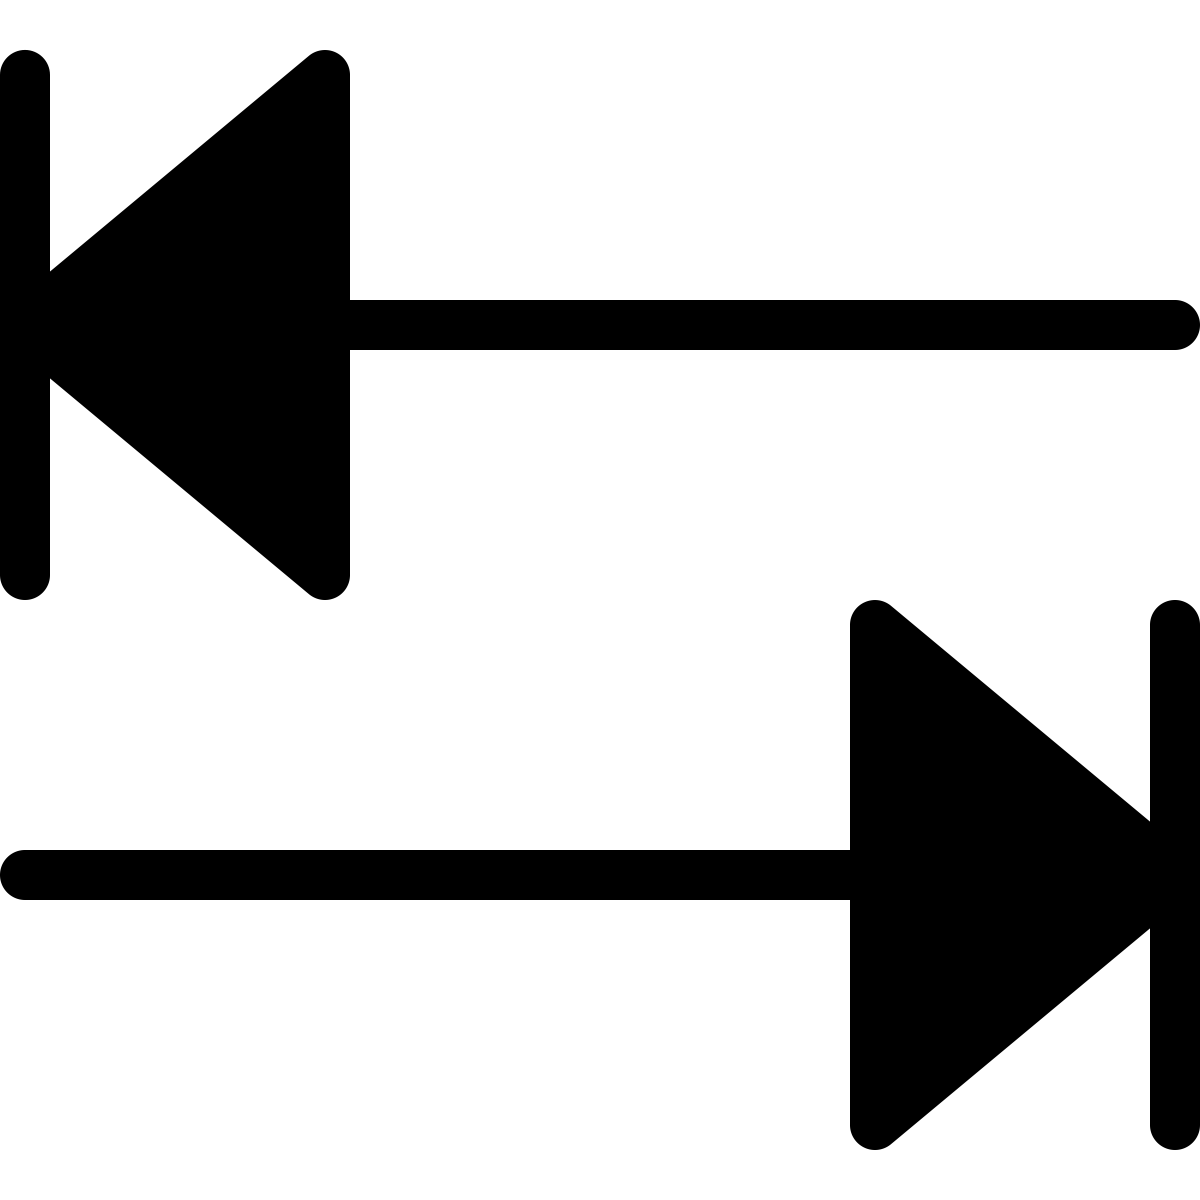
\includegraphics[width=0.15\textwidth,height=\textheight]{figures/tab_complete.png}

}

\end{figure}

Tab complete serves the following purposes:

\begin{enumerate}
\def\labelenumi{\arabic{enumi}.}
\tightlist
\item
  To complete path names and commands
\item
  To list all content that starts with what you have already typed
\item
  To ensure you have no typos
\end{enumerate}

In the below examples press the tab button when you see
\textbf{\textless tab\textgreater{}} and \textbf{replace 2xx with your
user number.}

Move into the directory \textbf{``1\_directory''}

\begin{Shaded}
\begin{Highlighting}[]
\BuiltInTok{cd}\NormalTok{ /pub14/t}\OperatorTok{\textless{}}\NormalTok{tab}\OperatorTok{\textgreater{}}\NormalTok{n}\OperatorTok{\textless{}}\NormalTok{tab}\OperatorTok{\textgreater{}}\NormalTok{2xx}\OperatorTok{\textless{}}\NormalTok{tab}\OperatorTok{\textgreater{}}\NormalTok{L}\OperatorTok{\textless{}}\NormalTok{tab}\OperatorTok{\textgreater{}}\NormalTok{1\_d}\OperatorTok{\textless{}}\NormalTok{tab}\OperatorTok{\textgreater{}}
\end{Highlighting}
\end{Shaded}

Print out all the content within the current directory that starts with
\textbf{``1\_''} in the file or directory name. This is carried out with
a double tab.

\textbf{Note}: the \textbf{``./''} is put before the 1 so it only looks
in the current directory otherwise it will also look for commands.

\begin{Shaded}
\begin{Highlighting}[]
\ExtensionTok{./1\_}\OperatorTok{\textless{}}\NormalTok{tab}\OperatorTok{\textgreater{}\textless{}}\NormalTok{tab}\OperatorTok{\textgreater{}}
\end{Highlighting}
\end{Shaded}

List the contents of directory \textbf{``1\_1\_directory''}

\begin{Shaded}
\begin{Highlighting}[]
\FunctionTok{ls}\NormalTok{ 1\_1}\OperatorTok{\textless{}}\NormalTok{tab}\OperatorTok{\textgreater{}}
\end{Highlighting}
\end{Shaded}

Change directory to \textbf{``1\_2\_directory''}. The \textbf{``./''} is
not needed before the file name as tab will only look for directories
because it is used for an argument of the \texttt{cd} command.

\begin{Shaded}
\begin{Highlighting}[]
\BuiltInTok{cd}\NormalTok{ 1\_2}\OperatorTok{\textless{}}\NormalTok{tab}\OperatorTok{\textgreater{}}
\end{Highlighting}
\end{Shaded}

Change directory to \textbf{example\_1\_part\_1}. The last tab will add
the \textbf{``/''} to the end of the directory name, this informs you
that you have correctly and fully typed in the directory name. However,
this will not always occur if there is another directory name that
starts the same but is longer. That is where double tab comes in handy.

\begin{Shaded}
\begin{Highlighting}[]
\BuiltInTok{cd}\NormalTok{ e}\OperatorTok{\textless{}}\NormalTok{tab}\OperatorTok{\textgreater{}}\NormalTok{1}\OperatorTok{\textless{}}\NormalTok{tab}\OperatorTok{\textgreater{}}\NormalTok{1}\OperatorTok{\textless{}}\NormalTok{tab}\OperatorTok{\textgreater{}}
\end{Highlighting}
\end{Shaded}

In this practical session I have given paths purposefully long names.
This has been carried out to demonstrate the usefulness of tab complete
and to encourage its use. Although they have been artificially extended
in this case, in Bioinformatics long and informative path names are
advised.

\hypertarget{ending-a-command}{%
\section{Ending a command}\label{ending-a-command}}

There are times when you will want to abandon a command on the command
line. To do this simple press \textbf{`Ctrl' + `c'}.

This is useful if a command won't respond or you noticed you have run a
command with a typo or with the wrong file.

\hypertarget{history}{%
\section{History}\label{history}}

\begin{figure}

{\centering 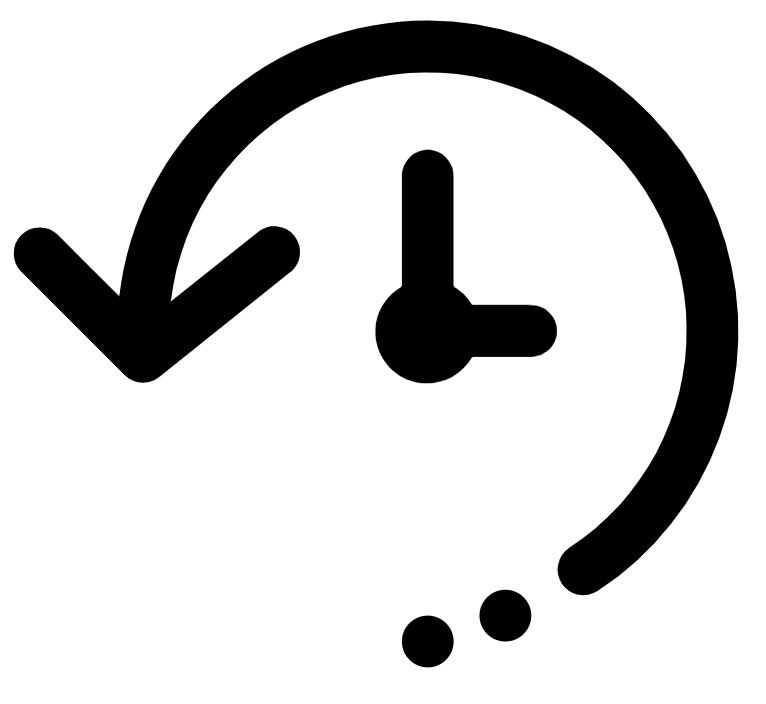
\includegraphics[width=0.15\textwidth,height=\textheight]{figures/history.png}

}

\end{figure}

Linux will save commands you have previously entered. In the terminal,
whilst at the command line, you can press the up and down keys to scroll
through your history. You can then rerun previous commands or edit them
with the left and right arrow keys, and run the edited version.

\hypertarget{clear}{%
\section{Clear}\label{clear}}

The \texttt{clear} command can be used to clear all the text from the
terminal. This is useful for keeping a tidy terminal.

\hypertarget{bash-escape}{%
\section{Bash escape}\label{bash-escape}}

To continue a command on a new line on the command line use the
backslash character, \textbf{\texttt{\textbackslash{}}}. When you press
\texttt{\textbackslash{}} followed by enter, the command will not run
and you will be on a new line on the command line. This can be useful
for clarity and for long commands. In the below example press ``enter''
after the end of a line.

Print to screen the term ``Hello universe, today is a very nice day.
Don't you think so?''

\begin{Shaded}
\begin{Highlighting}[]
\BuiltInTok{echo} \DataTypeTok{\textbackslash{}}
\NormalTok{“Hello universe, today is a very nice day. Don’t you think so}\PreprocessorTok{?}\NormalTok{”}
\end{Highlighting}
\end{Shaded}

Notice that there is a space before the \texttt{\textbackslash{}}. This
is because there needs to be a space between the echo and text to print
out. It is always recommended to use a space before a
\texttt{\textbackslash{}} to bash escape.

Bash escape is useful for this document as it will show if commands in
this document are separate commands or one command over multiple lines.

\hypertarget{annotations}{%
\section{Annotations}\label{annotations}}

\begin{figure}

{\centering 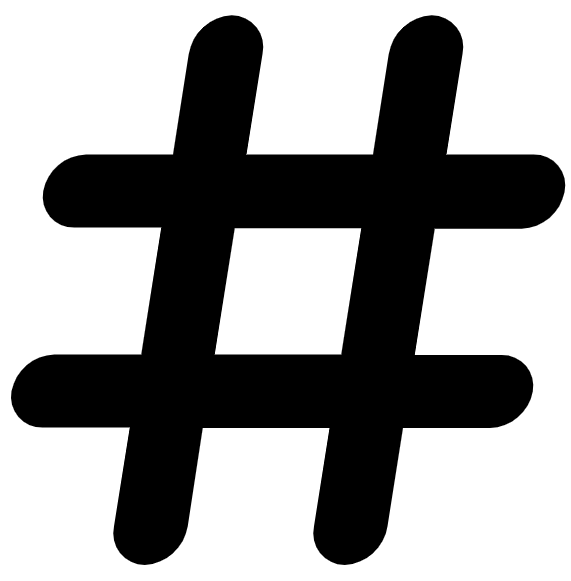
\includegraphics[width=0.15\textwidth,height=\textheight]{figures/hashtag.png}

}

\end{figure}

You can annotate your code so it will not run. This is carried out by
putting a \texttt{\#} at the start of a code line.

An example:

\begin{Shaded}
\begin{Highlighting}[]
\CommentTok{\#This line is annotation and will not run}
\CommentTok{\#The below line will print out the text "this line is not annotated"}
\BuiltInTok{echo} \StringTok{"this line is not annotated"}
\end{Highlighting}
\end{Shaded}

This is useful to give yourself information about what your code is
doing and it is vital if you are creating scripts. We will also use
annotations in this workbook to explain what some lines of code are
doing.

I also find it useful to put a \texttt{\#} at the front of a long
command that I am typing or editing. This means the command won't run if
I accidentally press enter. Just be sure to remove the \texttt{\#} at
the start of the line before you want to run it.

\hypertarget{mcqs-tips-tricks}{%
\section{MCQs: Tips \& tricks}\label{mcqs-tips-tricks}}

\begin{figure}

{\centering 
\includegraphics[width=0.2\textwidth,height=\textheight]{figures/question_bubble_blue.png}

}

\end{figure}

Please attempt to answer the below Multiple-Choice Questions to
reinforce what you have learnt in this chapter.

\begin{enumerate}
\def\labelenumi{\arabic{enumi}.}
\tightlist
\item
  What allows you to auto fill paths and commands so you can quickly
  type without error?
\end{enumerate}

\begin{itemize}
\item
  \begin{enumerate}
  \def\labelenumi{(\Alph{enumi})}
  \tightlist
  \item
    \textbf{\texttt{\#}}\strut \\
  \end{enumerate}
\item
  \begin{enumerate}
  \def\labelenumi{(\Alph{enumi})}
  \setcounter{enumi}{1}
  \tightlist
  \item
    \textbf{Tab complete}\\
  \end{enumerate}
\item
  \begin{enumerate}
  \def\labelenumi{(\Alph{enumi})}
  \setcounter{enumi}{2}
  \tightlist
  \item
    \textbf{\texttt{clear}}
  \end{enumerate}
\end{itemize}

\begin{enumerate}
\def\labelenumi{\arabic{enumi}.}
\setcounter{enumi}{1}
\tightlist
\item
  What command clears text from the terminal?
\end{enumerate}

\begin{itemize}
\item
  \begin{enumerate}
  \def\labelenumi{(\Alph{enumi})}
  \tightlist
  \item
    \textbf{\texttt{\#}}\strut \\
  \end{enumerate}
\item
  \begin{enumerate}
  \def\labelenumi{(\Alph{enumi})}
  \setcounter{enumi}{1}
  \tightlist
  \item
    \textbf{Tab complete}\\
  \end{enumerate}
\item
  \begin{enumerate}
  \def\labelenumi{(\Alph{enumi})}
  \setcounter{enumi}{2}
  \tightlist
  \item
    \textbf{\texttt{clear}}
  \end{enumerate}
\end{itemize}

\begin{enumerate}
\def\labelenumi{\arabic{enumi}.}
\setcounter{enumi}{2}
\tightlist
\item
  What symbol is used for annotation?
\end{enumerate}

\begin{itemize}
\item
  \begin{enumerate}
  \def\labelenumi{(\Alph{enumi})}
  \tightlist
  \item
    \textbf{\texttt{\#}}\strut \\
  \end{enumerate}
\item
  \begin{enumerate}
  \def\labelenumi{(\Alph{enumi})}
  \setcounter{enumi}{1}
  \tightlist
  \item
    \textbf{Tab complete}\\
  \end{enumerate}
\item
  \begin{enumerate}
  \def\labelenumi{(\Alph{enumi})}
  \setcounter{enumi}{2}
  \tightlist
  \item
    \textbf{\texttt{clear}}
  \end{enumerate}
\end{itemize}

\begin{enumerate}
\def\labelenumi{\arabic{enumi}.}
\setcounter{enumi}{3}
\tightlist
\item
  What keyboard short cut cancels/ends a command?
\end{enumerate}

\begin{itemize}
\item
  \begin{enumerate}
  \def\labelenumi{(\Alph{enumi})}
  \tightlist
  \item
    \textbf{Ctrl + c}\\
  \end{enumerate}
\item
  \begin{enumerate}
  \def\labelenumi{(\Alph{enumi})}
  \setcounter{enumi}{1}
  \tightlist
  \item
    \textbf{\texttt{\textbackslash{}}}\strut \\
  \end{enumerate}
\item
  \begin{enumerate}
  \def\labelenumi{(\Alph{enumi})}
  \setcounter{enumi}{2}
  \tightlist
  \item
    \textbf{Up and down arrow}
  \end{enumerate}
\end{itemize}

\begin{enumerate}
\def\labelenumi{\arabic{enumi}.}
\setcounter{enumi}{4}
\tightlist
\item
  What keys scroll through your previously run commands (aka history)?
\end{enumerate}

\begin{itemize}
\item
  \begin{enumerate}
  \def\labelenumi{(\Alph{enumi})}
  \tightlist
  \item
    \textbf{Ctrl + c}\\
  \end{enumerate}
\item
  \begin{enumerate}
  \def\labelenumi{(\Alph{enumi})}
  \setcounter{enumi}{1}
  \tightlist
  \item
    \textbf{\texttt{\textbackslash{}}}\strut \\
  \end{enumerate}
\item
  \begin{enumerate}
  \def\labelenumi{(\Alph{enumi})}
  \setcounter{enumi}{2}
  \tightlist
  \item
    \textbf{Up and down arrows}
  \end{enumerate}
\end{itemize}

\begin{enumerate}
\def\labelenumi{\arabic{enumi}.}
\setcounter{enumi}{5}
\tightlist
\item
  Bash escape allows you to run commands over multiple lines. What
  symbol is used for bash escape?
\end{enumerate}

\begin{itemize}
\item
  \begin{enumerate}
  \def\labelenumi{(\Alph{enumi})}
  \tightlist
  \item
    \textbf{Ctrl + c}\\
  \end{enumerate}
\item
  \begin{enumerate}
  \def\labelenumi{(\Alph{enumi})}
  \setcounter{enumi}{1}
  \tightlist
  \item
    \textbf{\texttt{\textbackslash{}}}\strut \\
  \end{enumerate}
\item
  \begin{enumerate}
  \def\labelenumi{(\Alph{enumi})}
  \setcounter{enumi}{2}
  \tightlist
  \item
    \textbf{Up and down arrow}
  \end{enumerate}
\end{itemize}

\hypertarget{manipulatingdirectories}{%
\chapter{Manipulating directories}\label{manipulatingdirectories}}

\begin{figure}

{\centering 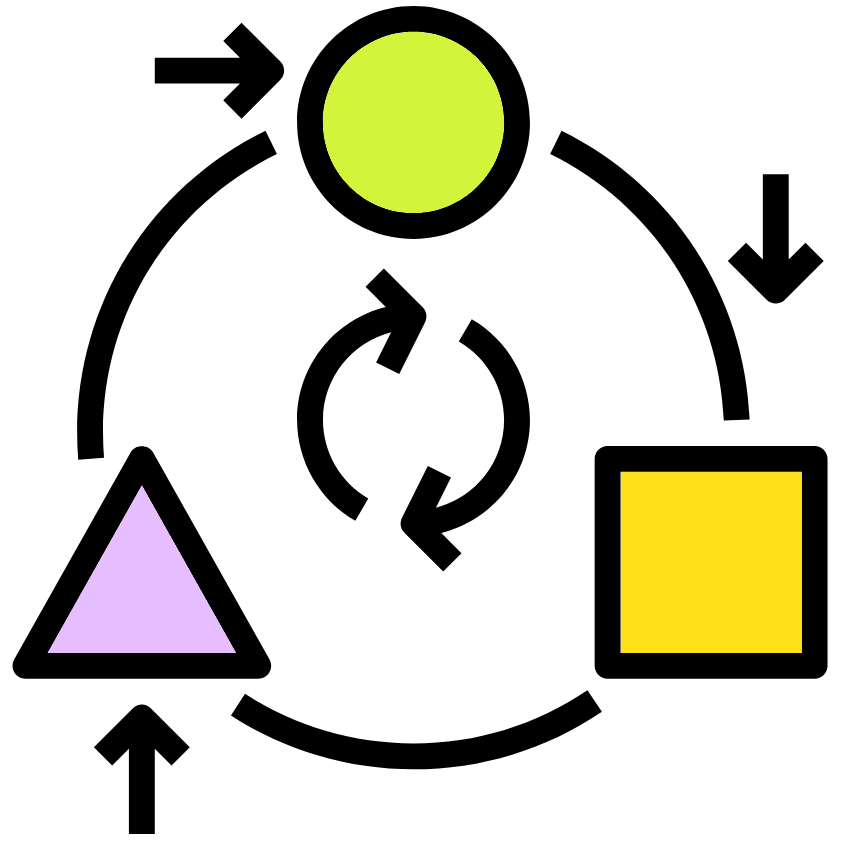
\includegraphics[width=0.2\textwidth,height=\textheight]{figures/transform.png}

}

\end{figure}

Chapter 6 video walk-through

\hypertarget{make-a-directory}{%
\section{Make a directory}\label{make-a-directory}}

To make a directory the command \texttt{mkdir} is used.

For the below examples we will be making heavy use of \texttt{ls} so you
can hopefully visualise the contents of the directories.

Type in the following commands to make a subdirectory within the
\textbf{``CGR\_Linux''} directory called \textbf{``Chicken''} then make
a subdirectory within \textbf{``Chicken''} called \textbf{``Egg''}.

\begin{Shaded}
\begin{Highlighting}[]
\CommentTok{\#Change directory to CGR\_linux in your home (\textasciitilde{})}
\BuiltInTok{cd}\NormalTok{ \textasciitilde{}/Linux/}
\CommentTok{\#Always good to list contents when you move into a directory}
\FunctionTok{ls}
\CommentTok{\#Make a directory called Chicken in your current directory}
\FunctionTok{mkdir}\NormalTok{ Chicken}
\CommentTok{\#Make a subdirectory of Chicken called Egg}
\FunctionTok{mkdir}\NormalTok{ Chicken/Egg}
\CommentTok{\#List the contents of the Chicken directory}
\FunctionTok{ls}\NormalTok{ Chicken}
\end{Highlighting}
\end{Shaded}

\textbf{Tip}: You can use the up arrow key to get to previously run
commands which you can edit using the right and left keys.

\hypertarget{moving-directories-and-files}{%
\section{Moving Directories and
Files}\label{moving-directories-and-files}}

\begin{figure}

{\centering 
\includegraphics[width=0.2\textwidth,height=\textheight]{figures/chicken.png}

}

\end{figure}

Files and directories can be moved with the \texttt{mv} command. This
can also be used to change the name of a file or a directory.

\textbf{Note}: If you move a file to the path of a file that already
exists, the pre existing file will be overwritten.

First ensure your working directory is the \textbf{``Linux''} directory.

Move the \textbf{``Chicken''} directory into the
\textbf{``3\_chicken\_farm/3\_1\_hut/''} directory. This will move the
directory and all its contents.

\begin{Shaded}
\begin{Highlighting}[]
\CommentTok{\#Before moving list the contents of the the destination directory}
\FunctionTok{ls}\NormalTok{ 3\_chicken\_farm/3\_1\_hut/}
\CommentTok{\#Also list the contents of the current directory to ensure }
\CommentTok{\#Chicken is present}
\FunctionTok{ls}
\CommentTok{\#Move Chicken to 3\_chicken\_farm/3\_1\_hut/}
\FunctionTok{mv}\NormalTok{ Chicken/ 3\_chicken\_farm/3\_1\_hut/}
\CommentTok{\#List the current directory and destination}
\FunctionTok{ls}\NormalTok{ . 3\_chicken\_farm/3\_1\_hut/}
\end{Highlighting}
\end{Shaded}

Move the Directory \textbf{``3\_chicken\_farm/3\_1\_hut/Chicken/''} to
\textbf{``3\_chicken\_farm/3\_2\_field''} and rename it
\textbf{``Outdoor\_Chicken''}.

\begin{Shaded}
\begin{Highlighting}[]
\CommentTok{\#List the contents of the start directory}
\FunctionTok{ls}\NormalTok{ \textasciitilde{}/Linux/3\_chicken\_farm/3\_1\_hut}
\CommentTok{\#Move the Chicken directory whilst renaming it}
\FunctionTok{mv}\NormalTok{ \textasciitilde{}/Linux/3\_chicken\_farm/3\_1\_hut/Chicken/ }\DataTypeTok{\textbackslash{}}
\NormalTok{\textasciitilde{}/Linux/3\_chicken\_farm/3\_2\_field/Outdoor\_Chicken}
\CommentTok{\#List the contents of the destination directory}
\FunctionTok{ls}\NormalTok{ \textasciitilde{}/Linux/3\_chicken\_farm/3\_2\_field/Outdoor\_Chicken}
\end{Highlighting}
\end{Shaded}

Move the file \textbf{``3\_chicken\_farm/3\_3\_supplies/feed.txt''} to
the directory \textbf{``3\_chicken\_farm/3\_2\_field''} and rename it
\textbf{``used\_feed.txt''}

\begin{Shaded}
\begin{Highlighting}[]
\CommentTok{\#List start directory to see if the feed.txt file exists}
\FunctionTok{ls}\NormalTok{ 3\_chicken\_farm/3\_3\_supplies/feed.txt}
\CommentTok{\#Move and rename the feed.txt file}
\FunctionTok{mv}\NormalTok{ 3\_chicken\_farm/3\_3\_supplies/feed.txt }\DataTypeTok{\textbackslash{}}
\NormalTok{3\_chicken\_farm/3\_2\_field/used\_feed.txt}
\CommentTok{\#List destination directory}
\FunctionTok{ls}\NormalTok{ 3\_chicken\_farm/3\_2\_field/}
\end{Highlighting}
\end{Shaded}

\hypertarget{copying-directories-and-files}{%
\section{Copying Directories and
Files}\label{copying-directories-and-files}}

\begin{figure}

{\centering 
\includegraphics[width=0.2\textwidth,height=\textheight]{figures/copy.png}

}

\end{figure}

Files and directories can be copied with the \texttt{cp} command.
Directories and files can be copied to any directory and given a new
name. Note: If you copy a file to the path of a file that already
exists, the pre existing file will be overwritten.

Before running the below commands move into your
\textbf{``\textasciitilde/Linux/3\_chicken\_farm/''} directory.

\begin{Shaded}
\begin{Highlighting}[]
\CommentTok{\#Change directory}
\BuiltInTok{cd}\NormalTok{ \textasciitilde{}/Linux/3\_chicken\_farm/}
\CommentTok{\#List contents of current directory}
\FunctionTok{ls}
\end{Highlighting}
\end{Shaded}

Copy the file \textbf{``3\_1\_hut/Laid\_Egg.txt''} to the
\textbf{``3\_2\_field''} directory and give it the filename
\textbf{``Chick.txt''}

\begin{Shaded}
\begin{Highlighting}[]
\CommentTok{\#List contents of 3\_1\_hut}
\FunctionTok{ls}\NormalTok{ 3\_1\_hut}
\CommentTok{\#Copy Laid\_egg to another directory as a new file called Chick.txt}
\FunctionTok{cp}\NormalTok{ 3\_1\_hut/Laid\_Egg.txt 3\_2\_field/Chick.txt}
\CommentTok{\#List contents of 3\_2\_field}
\FunctionTok{ls}\NormalTok{ 3\_2\_field}
\end{Highlighting}
\end{Shaded}

Copy the file \textbf{``3\_2\_field/Chick.txt''} and give the copy the
name \textbf{``Chick\_2.txt''}

\begin{Shaded}
\begin{Highlighting}[]
\CommentTok{\#List contents of 3\_2\_field}
\FunctionTok{ls}\NormalTok{ 3\_2\_field}
\CommentTok{\#Copy the Chick.txt file as Chick\_2.txt}
\FunctionTok{cp}\NormalTok{ 3\_2\_field/Chick.txt 3\_2\_field/Chick\_2.txt}
\CommentTok{\#List contents of 3\_2\_field}
\FunctionTok{ls}\NormalTok{ 3\_2\_field}
\end{Highlighting}
\end{Shaded}

Copy the directory \textbf{``3\_1\_hut''} to \textbf{``3\_1\_hut\_2''}

\begin{Shaded}
\begin{Highlighting}[]
\CommentTok{\#List contents of current directory}
\FunctionTok{ls}
\CommentTok{\#Copy directory with {-}r (recursively)}
\FunctionTok{cp} \AttributeTok{{-}r}\NormalTok{ 3\_1\_hut 3\_1\_hut\_2}
\CommentTok{\#List contents of current directory}
\FunctionTok{ls}
\end{Highlighting}
\end{Shaded}

\hypertarget{deleting-files-and-directories}{%
\section{Deleting Files and
Directories}\label{deleting-files-and-directories}}

\begin{figure}

{\centering 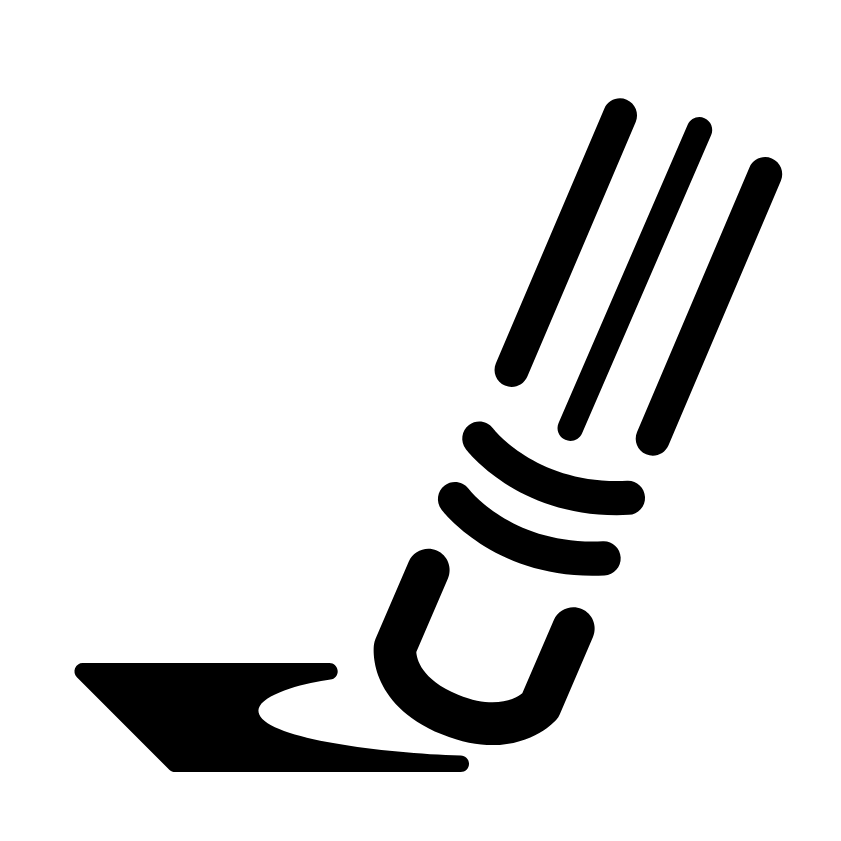
\includegraphics[width=0.2\textwidth,height=\textheight]{figures/erase.png}

}

\end{figure}

To delete files and directories the command \texttt{rm} can be used.

\textbf{Important}: This command can be very dangerous. There is no
recycle bin on Linux machines so once you delete something it cannot be
recovered. Be very careful when deleting files and directories. To avoid
major loss try to keep backups of important data and scripts.

Ensure you are in your \textbf{``3\_chicken\_farm/''} directory

Remove the file \textbf{``3\_2\_field/Chick\_2.txt''}

\begin{Shaded}
\begin{Highlighting}[]
\CommentTok{\#List contents of 3\_2\_field}
\FunctionTok{ls}\NormalTok{ 3\_2\_field}
\CommentTok{\#Remove Chick\_2.txt}
\FunctionTok{rm}\NormalTok{ 3\_2\_field/Chick\_2.txt}
\CommentTok{\#List contents of 3\_2\_field}
\FunctionTok{ls}\NormalTok{ 3\_2\_field}
\end{Highlighting}
\end{Shaded}

Remove the directory \textbf{``3\_1\_hut\_2/''} and its contents

\begin{Shaded}
\begin{Highlighting}[]
\CommentTok{\#List contents of current directory}
\FunctionTok{ls}
\CommentTok{\#Remove directory with {-}r (recursively)}
\FunctionTok{rm} \AttributeTok{{-}r}\NormalTok{  3\_1\_hut\_2}
\CommentTok{\#List contents of current directory}
\FunctionTok{ls}
\end{Highlighting}
\end{Shaded}

\hypertarget{mcqs-manipulating-directories}{%
\section{MCQs: Manipulating
directories}\label{mcqs-manipulating-directories}}

\begin{figure}

{\centering 
\includegraphics[width=0.2\textwidth,height=\textheight]{figures/question_bubble_green.png}

}

\end{figure}

Please attempt to answer the below Multiple-Choice Questions to
reinforce what you have learnt in this chapter.

\begin{enumerate}
\def\labelenumi{\arabic{enumi}.}
\tightlist
\item
  What command removes files and directories?
\end{enumerate}

\begin{itemize}
\item
  \begin{enumerate}
  \def\labelenumi{(\Alph{enumi})}
  \tightlist
  \item
    \textbf{\texttt{rm}}\strut \\
  \end{enumerate}
\item
  \begin{enumerate}
  \def\labelenumi{(\Alph{enumi})}
  \setcounter{enumi}{1}
  \tightlist
  \item
    \textbf{\texttt{mv}}\strut \\
  \end{enumerate}
\item
  \begin{enumerate}
  \def\labelenumi{(\Alph{enumi})}
  \setcounter{enumi}{2}
  \tightlist
  \item
    \textbf{\texttt{ls}}
  \end{enumerate}
\end{itemize}

\begin{enumerate}
\def\labelenumi{\arabic{enumi}.}
\setcounter{enumi}{1}
\tightlist
\item
  What command moves files and directories?
\end{enumerate}

\begin{itemize}
\item
  \begin{enumerate}
  \def\labelenumi{(\Alph{enumi})}
  \tightlist
  \item
    \textbf{\texttt{rm}}\strut \\
  \end{enumerate}
\item
  \begin{enumerate}
  \def\labelenumi{(\Alph{enumi})}
  \setcounter{enumi}{1}
  \tightlist
  \item
    \textbf{\texttt{mv}}\strut \\
  \end{enumerate}
\item
  \begin{enumerate}
  \def\labelenumi{(\Alph{enumi})}
  \setcounter{enumi}{2}
  \tightlist
  \item
    \textbf{\texttt{ls}}
  \end{enumerate}
\end{itemize}

\begin{enumerate}
\def\labelenumi{\arabic{enumi}.}
\setcounter{enumi}{2}
\tightlist
\item
  What command makes a new directory?
\end{enumerate}

\begin{itemize}
\item
  \begin{enumerate}
  \def\labelenumi{(\Alph{enumi})}
  \tightlist
  \item
    \textbf{\texttt{-r}}\strut \\
  \end{enumerate}
\item
  \begin{enumerate}
  \def\labelenumi{(\Alph{enumi})}
  \setcounter{enumi}{1}
  \tightlist
  \item
    \textbf{\texttt{mkdir}}\strut \\
  \end{enumerate}
\item
  \begin{enumerate}
  \def\labelenumi{(\Alph{enumi})}
  \setcounter{enumi}{2}
  \tightlist
  \item
    \textbf{\texttt{ls}}
  \end{enumerate}
\end{itemize}

\begin{enumerate}
\def\labelenumi{\arabic{enumi}.}
\setcounter{enumi}{3}
\tightlist
\item
  What option is needed for moving or removing a directory?
\end{enumerate}

\begin{itemize}
\item
  \begin{enumerate}
  \def\labelenumi{(\Alph{enumi})}
  \tightlist
  \item
    \textbf{\texttt{-r}}\strut \\
  \end{enumerate}
\item
  \begin{enumerate}
  \def\labelenumi{(\Alph{enumi})}
  \setcounter{enumi}{1}
  \tightlist
  \item
    \textbf{\texttt{mkdir}}\strut \\
  \end{enumerate}
\item
  \begin{enumerate}
  \def\labelenumi{(\Alph{enumi})}
  \setcounter{enumi}{2}
  \tightlist
  \item
    \textbf{\texttt{ls}}
  \end{enumerate}
\end{itemize}

\begin{enumerate}
\def\labelenumi{\arabic{enumi}.}
\setcounter{enumi}{4}
\tightlist
\item
  What command list the contents of directories?
\end{enumerate}

\begin{itemize}
\item
  \begin{enumerate}
  \def\labelenumi{(\Alph{enumi})}
  \tightlist
  \item
    \textbf{\texttt{-r}}\strut \\
  \end{enumerate}
\item
  \begin{enumerate}
  \def\labelenumi{(\Alph{enumi})}
  \setcounter{enumi}{1}
  \tightlist
  \item
    \textbf{\texttt{mkdir}}\strut \\
  \end{enumerate}
\item
  \begin{enumerate}
  \def\labelenumi{(\Alph{enumi})}
  \setcounter{enumi}{2}
  \tightlist
  \item
    \textbf{\texttt{ls}}
  \end{enumerate}
\end{itemize}

\hypertarget{exercise-1}{%
\chapter{Exercise 1}\label{exercise-1}}

\begin{figure}

{\centering 
\includegraphics[width=0.2\textwidth,height=\textheight]{figures/exercise.png}

}

\end{figure}

Perform the following tasks with the skills and knowledge you have
gained.

Change the name of the subdirectory \textbf{``four\_exercises''} within
your \textbf{``Linux''} directory to \textbf{``4\_exercises''}

\begin{enumerate}
\def\labelenumi{\arabic{enumi}.}
\tightlist
\item
  Make a backup of the \textbf{``4\_exercises''} directory
\item
  List the contents of the \textbf{``4\_exercises''} directory
\item
  Within the directory \textbf{``4\_exercises''}

  \begin{enumerate}
  \def\labelenumii{\arabic{enumii}.}
  \tightlist
  \item
    Print the working directory.
  \item
    Print out to screen the phrase `\textbf{the echo command allows me
    to print phrases to screen}'.
  \item
    Copy the file \textbf{``copy\_this\_file.txt''} to the directory
    \textbf{``to\_me''}
  \item
    Rename the directory \textbf{``to\_me''} to \textbf{``you''}
  \item
    Delete the initial \textbf{``copy\_this\_file.txt''} file
  \end{enumerate}
\end{enumerate}

You can check my solutions in the
\protect\hyperlink{exercise1_answers}{Answers section}. These are not
the definitive solution but only examples of solutions. If your method
works and you understand why then you have done it correctly.

\part{Part 2}

\hypertarget{filereadingandprocessing}{%
\chapter{File reading and processing}\label{filereadingandprocessing}}

\begin{figure}

{\centering 
\includegraphics[width=0.2\textwidth,height=\textheight]{figures/files.png}

}

\end{figure}

There are many ways to show the contents of a file. Below are a few
examples.

The files for the examples are within the directory:
\textbf{``/pub14/tea/nsc2xx/Linux/5\_reading\_files/''} \textbf{(replace
xxx with your user number)}.

Chapter 8 video walk-through

\hypertarget{print-out-a-file}{%
\section{Print out a file}\label{print-out-a-file}}

\begin{figure}

{\centering 
\includegraphics[width=0.2\textwidth,height=\textheight]{figures/cat.png}

}

\end{figure}

The \texttt{cat} command will print out the entire contents of a file to
the screen. This is useful for small text files and pipelines (pipelines
are not covered here). Example commands are below (remember to replace
xxx with your user name number):

\textbf{Note}: remember tab complete and using the arrow keys

Print contents of \textbf{``short\_file.txt''} to screen

\begin{Shaded}
\begin{Highlighting}[]
\FunctionTok{cat}\NormalTok{ /pub14/tea/nsc2xx/Linux/5\_reading\_files/short\_file.txt}
\end{Highlighting}
\end{Shaded}

Print contents of \textbf{``Scientist.txt''} to screen

\begin{Shaded}
\begin{Highlighting}[]
\FunctionTok{cat}\NormalTok{ /pub14/tea/nsc2xx/Linux/5\_reading\_files/Scientist.txt}
\end{Highlighting}
\end{Shaded}

Print contents of \textbf{``ecoli.gbk''} to screen

\begin{Shaded}
\begin{Highlighting}[]
\FunctionTok{cat}\NormalTok{ /pub14/tea/nsc2xx/Linux/5\_reading\_files/ecoli.gbk}
\end{Highlighting}
\end{Shaded}

\textbf{Remember}: The \texttt{clear} command.

\hypertarget{head-and-tail}{%
\section{head and tail}\label{head-and-tail}}

\begin{figure}

{\centering 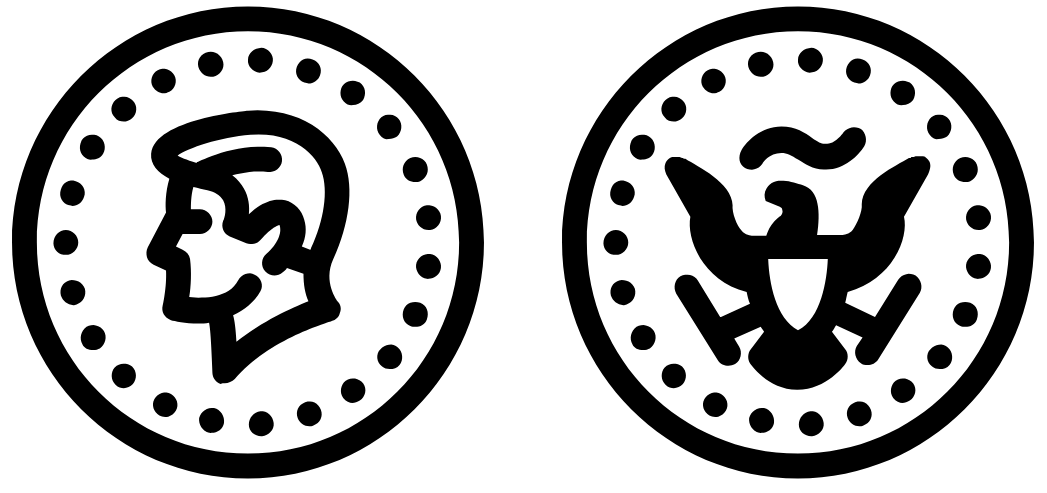
\includegraphics[width=0.3\textwidth,height=\textheight]{figures/head_and_tails.png}

}

\end{figure}

The \texttt{head} command will print out to screen the top n lines of a
file.

The \texttt{tail} command will print out to screen the bottom n lines of
a file.

The default value is 10. The \texttt{-n} option can be used to indicate
how many lines to print out.

Carry out the below commands in the directory
\textbf{``/pub14/tea/nsc2xx/Linux/5\_reading\_files/''}

Print out the top 10 lines of \textbf{``ecoli.gbk''}

\begin{Shaded}
\begin{Highlighting}[]
\FunctionTok{head}\NormalTok{ ecoli.gbk}
\end{Highlighting}
\end{Shaded}

Print out the bottom 10 lines of \textbf{``ecoli.gbk''}

\begin{Shaded}
\begin{Highlighting}[]
\FunctionTok{tail}\NormalTok{ ecoli.gbk}
\end{Highlighting}
\end{Shaded}

Print out the top 25 lines of \textbf{``ecoli.gbk''}

\begin{Shaded}
\begin{Highlighting}[]
\FunctionTok{head} \AttributeTok{{-}n}\NormalTok{ 25 ecoli.gbk}
\end{Highlighting}
\end{Shaded}

Print out the bottom 2 lines of \textbf{``ecoli.gbk''}

\begin{Shaded}
\begin{Highlighting}[]
\FunctionTok{tail} \AttributeTok{{-}n}\NormalTok{ 2 ecoli.gbk}
\end{Highlighting}
\end{Shaded}

Print out all but the bottom 2 lines of \textbf{``Scientist.txt''}

\begin{Shaded}
\begin{Highlighting}[]
\FunctionTok{head} \AttributeTok{{-}n} \AttributeTok{{-}2}\NormalTok{ Scientist.txt}
\end{Highlighting}
\end{Shaded}

Print out all lines starting from the 2nd top line of
\textbf{``Scientist.txt''}

\begin{Shaded}
\begin{Highlighting}[]
\FunctionTok{tail} \AttributeTok{{-}n}\NormalTok{ +2 Scientist.txt}
\end{Highlighting}
\end{Shaded}

Print out all but the bottom 5 lines of \textbf{``Scientist.txt''}

\begin{Shaded}
\begin{Highlighting}[]
\FunctionTok{head} \AttributeTok{{-}n} \AttributeTok{{-}5}\NormalTok{ Scientist.txt}
\end{Highlighting}
\end{Shaded}

Print out all lines starting from the 3rd top line of
\textbf{``Scientist.txt''}

\begin{Shaded}
\begin{Highlighting}[]
\FunctionTok{tail} \AttributeTok{{-}n}\NormalTok{ +3 Scientist.txt}
\end{Highlighting}
\end{Shaded}

Print out the top 25 lines of \textbf{``ecoli.gbk''}

\begin{Shaded}
\begin{Highlighting}[]
\FunctionTok{head} \AttributeTok{{-}n}\NormalTok{ +25 ecoli.gbk}
\end{Highlighting}
\end{Shaded}

Print out the bottom 2 lines of \textbf{``ecoli.gbk''}

\begin{Shaded}
\begin{Highlighting}[]
\FunctionTok{tail} \AttributeTok{{-}n} \AttributeTok{{-}2}\NormalTok{ ecoli.gbk}
\end{Highlighting}
\end{Shaded}

\hypertarget{file-viewing-with-less}{%
\section{File viewing with less}\label{file-viewing-with-less}}

\begin{figure}

{\centering 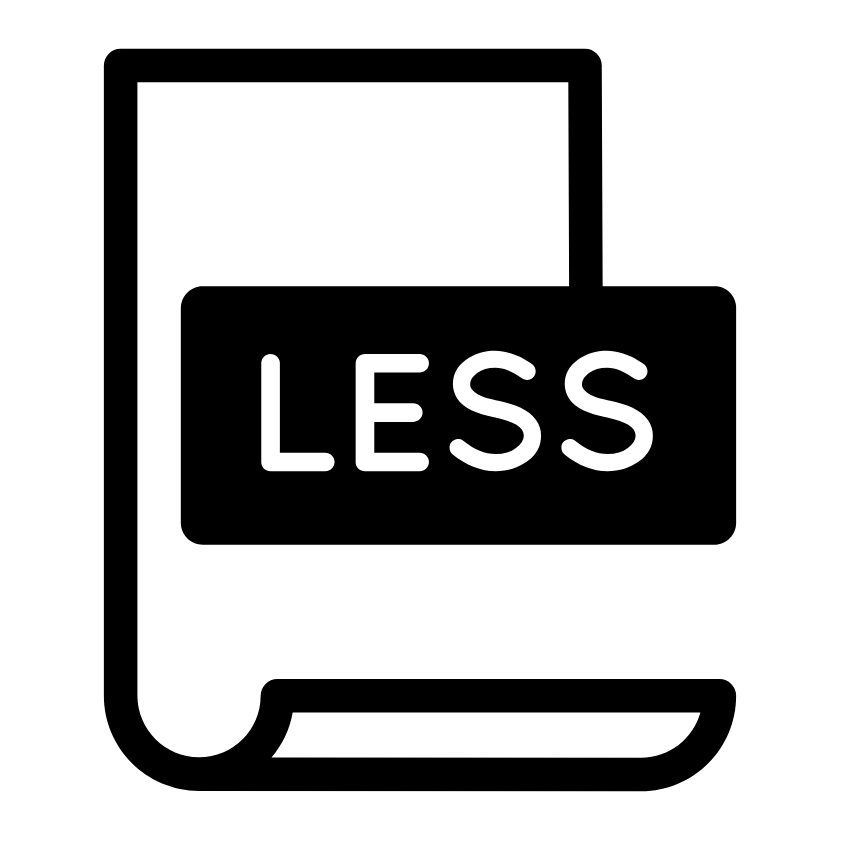
\includegraphics[width=0.2\textwidth,height=\textheight]{figures/less.png}

}

\end{figure}

The \texttt{less} command will display a file's contents one page at a
time. Various keys on the keyboard will allow you to navigate the
contents of the files. The below actions will occur identically with the
man command.

\begin{itemize}
\tightlist
\item
  \textbf{q} : Exit
\item
  \textbf{up and down arrow keys} : Will move up/down 1 line at a time
\item
  \textbf{space} : Move down one page
\item
  \textbf{b} : Move up one page
\item
  \textbf{\texttt{/}} : Follow this by a term to search for it in the
  file's contents
\item
  \textbf{n} : Find the next occurrence of the term last searched for
\item
  \textbf{N} : Find the previous occurrence of the term last searched
  for
\item
  \textbf{g} : Jump to the first line of the file
\item
  \textbf{G} : Jump to the bottom line of the file
\end{itemize}

Use the \texttt{less} command to view the contents of the
\textbf{``ecoli.gbk''} file. Then find the 3rd occurrence of the word
`ribosome'. Afterwards move around the file.

\begin{Shaded}
\begin{Highlighting}[]
\FunctionTok{less}\NormalTok{ ecoli.gbk}
\end{Highlighting}
\end{Shaded}

Look at the \texttt{man}ual for \texttt{less} and search for the first
occurrence of the string `percent'. Afterwards look around the manual
page.

\begin{Shaded}
\begin{Highlighting}[]
\FunctionTok{man}\NormalTok{ less}
\end{Highlighting}
\end{Shaded}

\hypertarget{word-count}{%
\section{Word count}\label{word-count}}

\begin{figure}

{\centering 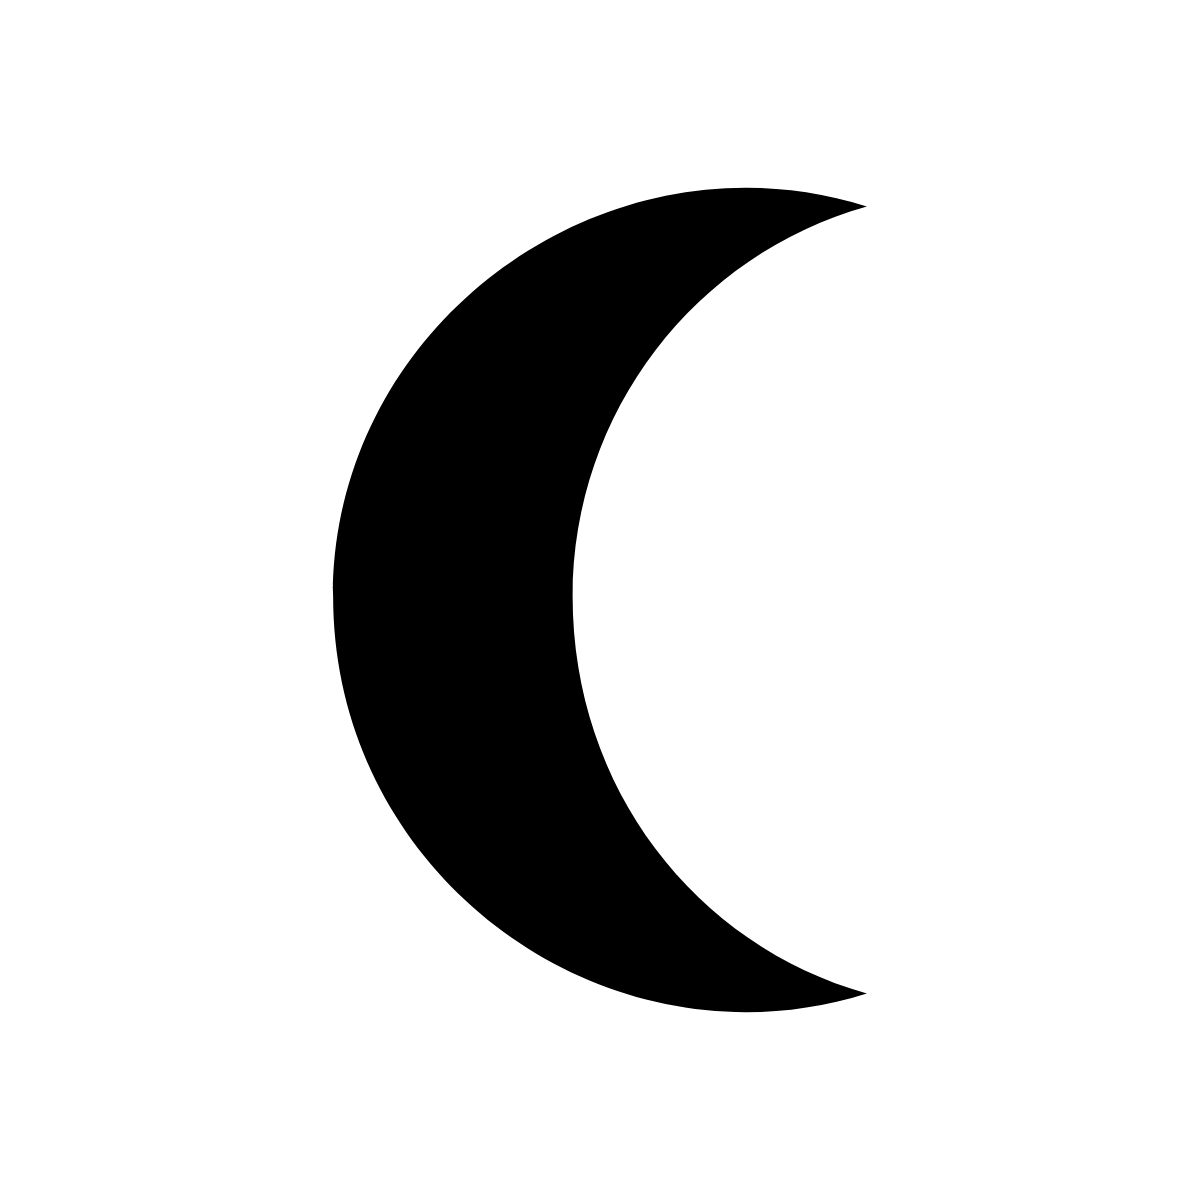
\includegraphics[width=0.2\textwidth,height=\textheight]{figures/wc.png}

}

\end{figure}

The \texttt{wc} command will allow allow you to word count files. It
will display line, word and byte counts for files in that order.

Use \texttt{wc} to see the line, word and byte count of the
\textbf{``short\_file.txt''} and \textbf{``ecoli.gbk''} files. As you
can see you can carry this out on multiple files at once.

\begin{Shaded}
\begin{Highlighting}[]
\FunctionTok{wc}\NormalTok{ short\_file.txt Scientist.txt ecoli.gbk}
\end{Highlighting}
\end{Shaded}

Count the number of characters in the \textbf{``short\_file.txt''} file

\begin{Shaded}
\begin{Highlighting}[]
\FunctionTok{wc} \AttributeTok{{-}m}\NormalTok{ short\_file.txt}
\end{Highlighting}
\end{Shaded}

Count the number of lines in the \textbf{``ecoli.gbk''} file

\begin{Shaded}
\begin{Highlighting}[]
\FunctionTok{wc} \AttributeTok{{-}l}\NormalTok{ ecoli.gbk}
\end{Highlighting}
\end{Shaded}

\hypertarget{pattern-searching}{%
\section{Pattern searching}\label{pattern-searching}}

\begin{figure}

{\centering 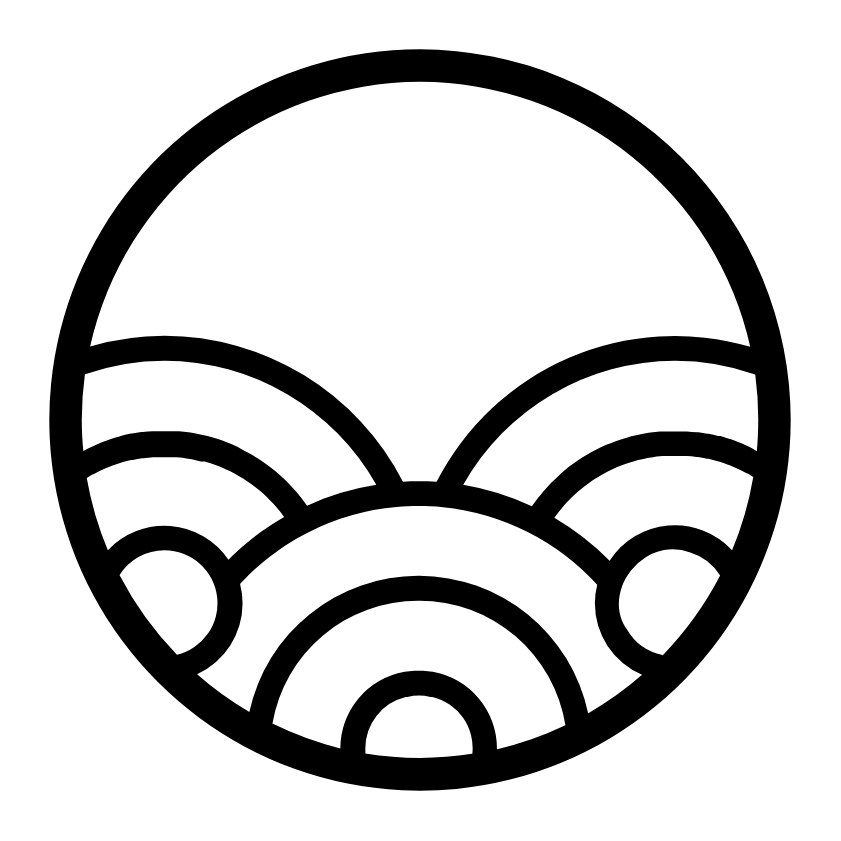
\includegraphics[width=0.2\textwidth,height=\textheight]{figures/pattern.png}

}

\end{figure}

The \texttt{grep} command will search for a pattern in a text file and
output all the lines containing the pattern.

Print out the lines from \textbf{``Scientist.txt''} that have the number
18 in them. In this particular example it prints out all scientists
which were born in the 1800s. This will not always be the case depending
on the data in the file.

\begin{Shaded}
\begin{Highlighting}[]
\FunctionTok{grep}\NormalTok{ “18” Scientist.txt}
\end{Highlighting}
\end{Shaded}

Print out the lines which have the string ``Ada'' in them.

\begin{Shaded}
\begin{Highlighting}[]
\FunctionTok{grep}\NormalTok{ “Ada” Scientist.txt}
\end{Highlighting}
\end{Shaded}

Print out the lines which have the string ``ada'' in them. There should
be none, as grep is case sensitive.

\begin{Shaded}
\begin{Highlighting}[]
\FunctionTok{grep}\NormalTok{ “ada” Scientist.txt}
\end{Highlighting}
\end{Shaded}

Type in the following command.

\begin{Shaded}
\begin{Highlighting}[]
\FunctionTok{grep}\NormalTok{ Scientist.txt}
\end{Highlighting}
\end{Shaded}

The above command will be stuck as \texttt{grep} does not know what it
is looking for. To cancel the command use \textbf{`Ctrl' + `c'}

\hypertarget{text-editor}{%
\section{Text editor}\label{text-editor}}

\begin{figure}

{\centering 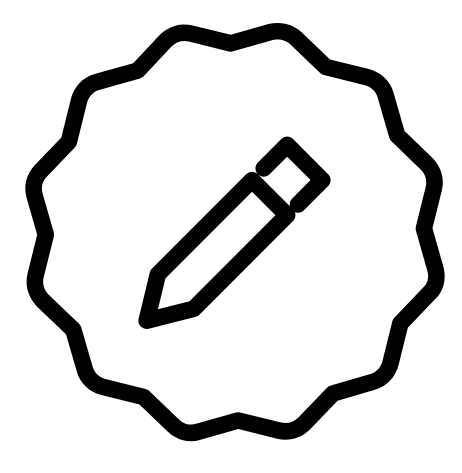
\includegraphics[width=0.2\textwidth,height=\textheight]{figures/text_editor.png}

}

\end{figure}

Three of the most popular text editors are \textbf{vim}, \textbf{gedit}
and \textbf{nano}. Below are quick introductions to \textbf{nano} and
\textbf{vim}.

\textbf{nano} is the easiest to learn but is quite limiting.
\textbf{vim} and \textbf{gedit} are quite similar in power with
different people preferring one or the other.

The below will teach you \textbf{nano}. If you are interested in
learning \textbf{vim} in the future you can find a quick guide in the
\protect\hyperlink{vim}{appendix}.

\hypertarget{nano}{%
\subsection{nano}\label{nano}}

\begin{figure}

{\centering 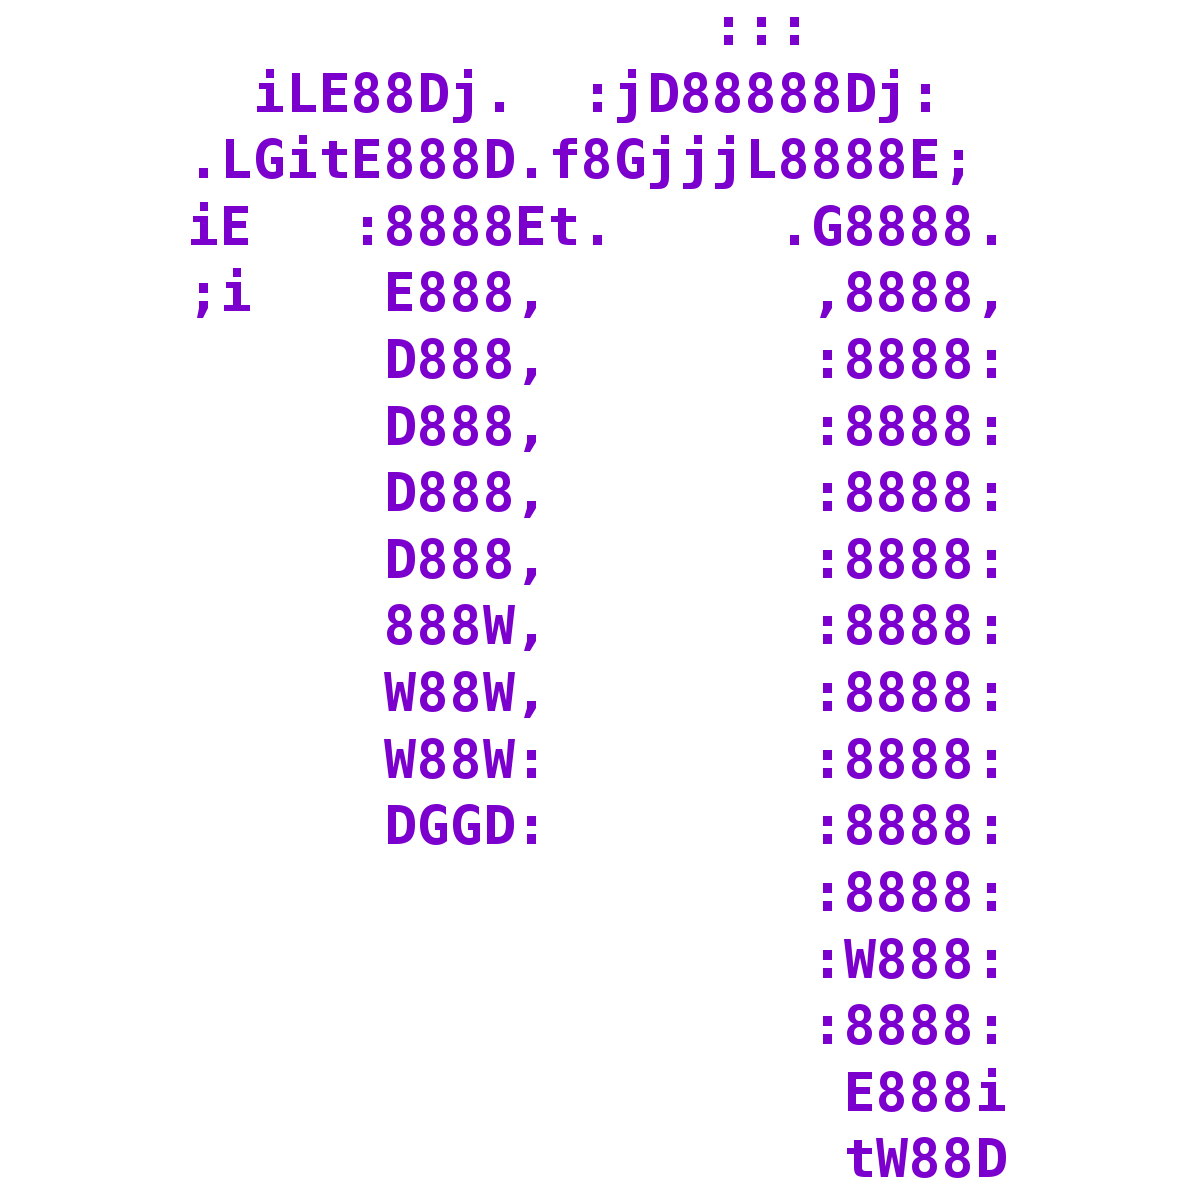
\includegraphics[width=0.2\textwidth,height=\textheight]{figures/1200px-Gnu-nano.png}

}

\end{figure}

To enter the \texttt{nano} text editor you can use the command
\texttt{nano}. The command is: \texttt{nano\ file.txt}.

\texttt{nano} can be run with a previous file name which you can then
edit or a new file name in which case you will create a new file.

Once you are in the editor you can type characters and move around with
the arrow keys.

To carry out specific functions you will need to use \textbf{Ctrl} or
\textbf{Alt} with another key. At the bottom of the editor are a few
examples where the \texttt{\^{}} indicates \textbf{Ctrl}. For example
the \texttt{\^{}G\ Get\ Help} means you need to press \textbf{Ctrl+G} to
get help. When you use letters this way in \textbf{nano} they are case
insensitive (i.e.~the CAPS lock can be on or off and you will get the
same result).

After you carry out a function ensure you look at the bottom of the
editor again as it may ask you to type something or you may get a new
series of functions you can use.

Below are some important examples:

\begin{itemize}
\tightlist
\item
  \textbf{Ctrl+X} - Exit nano
\item
  \textbf{Ctrl+S} - Save file
\item
  \textbf{Ctrl+O} - Save file as
\item
  \textbf{Ctrl+A} - Jump to the start of a line
\item
  \textbf{Ctrl+E} - Jump to the end of a line
\item
  \textbf{Ctrl+W} - Start search (Where is) \textbf{Note} This
  unfortunately is also the shortcut to close a tab in internet
  browsers. Therefore this can't be used with our webVNC.
\item
  \textbf{Alt+W} - Continue search forward (find next occurrence
  forward)
\item
  \textbf{Alt+Q} - Find next occurrence backward
\item
  \textbf{Alt+K} - Cut current line
\item
  \textbf{Alt+\textbackslash{}} - Go to the first line
\item
  \textbf{Alt+/} - Go to the last line
\end{itemize}

\href{https://www.nano-editor.org/dist/latest/cheatsheet.html}{\textbf{Nano
cheatsheet}}

\hypertarget{tasks}{%
\subsection{Tasks}\label{tasks}}

Carry out the following tasks in the directory:
\textbf{``/pub14/tea/nscxx/Linux/5\_reading\_files/''}

Using a text editor (\textbf{nano} or \textbf{vim}) add an entry for
Scientist Mae Jemison (Born: 1956) to the file
\textbf{``Scientist.txt''}. The names and date are separated by one tab.

Using your text editor of choice delete all the scientists born before
1000 in the \textbf{``Scientist.txt''} file and save this as
\textbf{``Scientist\_post\_1000.txt''}.

\hypertarget{mcqs-file-reading-and-processing}{%
\section{MCQs: File reading and
processing}\label{mcqs-file-reading-and-processing}}

\begin{figure}

{\centering 
\includegraphics[width=0.2\textwidth,height=\textheight]{figures/question_bubble_purple.png}

}

\end{figure}

Please attempt to answer the below Multiple-Choice Questions to
reinforce what you have learnt in this chapter.

\begin{enumerate}
\def\labelenumi{\arabic{enumi}.}
\tightlist
\item
  What command searches for a pattern?
\end{enumerate}

\begin{itemize}
\item
  \begin{enumerate}
  \def\labelenumi{(\Alph{enumi})}
  \tightlist
  \item
    \textbf{\texttt{wc}}\strut \\
  \end{enumerate}
\item
  \begin{enumerate}
  \def\labelenumi{(\Alph{enumi})}
  \setcounter{enumi}{1}
  \tightlist
  \item
    \textbf{\texttt{grep}}\strut \\
  \end{enumerate}
\item
  \begin{enumerate}
  \def\labelenumi{(\Alph{enumi})}
  \setcounter{enumi}{2}
  \tightlist
  \item
    \textbf{\texttt{cat}}
  \end{enumerate}
\end{itemize}

\begin{enumerate}
\def\labelenumi{\arabic{enumi}.}
\setcounter{enumi}{1}
\tightlist
\item
  What command word counts files?
\end{enumerate}

\begin{itemize}
\item
  \begin{enumerate}
  \def\labelenumi{(\Alph{enumi})}
  \tightlist
  \item
    \textbf{\texttt{wc}}\strut \\
  \end{enumerate}
\item
  \begin{enumerate}
  \def\labelenumi{(\Alph{enumi})}
  \setcounter{enumi}{1}
  \tightlist
  \item
    \textbf{\texttt{grep}}\strut \\
  \end{enumerate}
\item
  \begin{enumerate}
  \def\labelenumi{(\Alph{enumi})}
  \setcounter{enumi}{2}
  \tightlist
  \item
    \textbf{\texttt{cat}}
  \end{enumerate}
\end{itemize}

\begin{enumerate}
\def\labelenumi{\arabic{enumi}.}
\setcounter{enumi}{2}
\tightlist
\item
  What command prints the contents of a file?
\end{enumerate}

\begin{itemize}
\item
  \begin{enumerate}
  \def\labelenumi{(\Alph{enumi})}
  \tightlist
  \item
    \textbf{\texttt{wc}}\strut \\
  \end{enumerate}
\item
  \begin{enumerate}
  \def\labelenumi{(\Alph{enumi})}
  \setcounter{enumi}{1}
  \tightlist
  \item
    \textbf{\texttt{grep}}\strut \\
  \end{enumerate}
\item
  \begin{enumerate}
  \def\labelenumi{(\Alph{enumi})}
  \setcounter{enumi}{2}
  \tightlist
  \item
    \textbf{\texttt{cat}}
  \end{enumerate}
\end{itemize}

\begin{enumerate}
\def\labelenumi{\arabic{enumi}.}
\setcounter{enumi}{3}
\tightlist
\item
  What command displays a file's contents one page at a time and allows
  keyboard navigation?
\end{enumerate}

\begin{itemize}
\item
  \begin{enumerate}
  \def\labelenumi{(\Alph{enumi})}
  \tightlist
  \item
    \textbf{\texttt{less}}\strut \\
  \end{enumerate}
\item
  \begin{enumerate}
  \def\labelenumi{(\Alph{enumi})}
  \setcounter{enumi}{1}
  \tightlist
  \item
    \textbf{\texttt{tail}}\strut \\
  \end{enumerate}
\item
  \begin{enumerate}
  \def\labelenumi{(\Alph{enumi})}
  \setcounter{enumi}{2}
  \tightlist
  \item
    \textbf{\texttt{head}}
  \end{enumerate}
\end{itemize}

\begin{enumerate}
\def\labelenumi{\arabic{enumi}.}
\setcounter{enumi}{4}
\tightlist
\item
  What command prints out the top n lines of a file
\end{enumerate}

\begin{itemize}
\item
  \begin{enumerate}
  \def\labelenumi{(\Alph{enumi})}
  \tightlist
  \item
    \textbf{\texttt{less}}\strut \\
  \end{enumerate}
\item
  \begin{enumerate}
  \def\labelenumi{(\Alph{enumi})}
  \setcounter{enumi}{1}
  \tightlist
  \item
    \textbf{\texttt{tail}}\strut \\
  \end{enumerate}
\item
  \begin{enumerate}
  \def\labelenumi{(\Alph{enumi})}
  \setcounter{enumi}{2}
  \tightlist
  \item
    \textbf{\texttt{head}}
  \end{enumerate}
\end{itemize}

\begin{enumerate}
\def\labelenumi{\arabic{enumi}.}
\setcounter{enumi}{5}
\tightlist
\item
  What command prints out the bottom n lines of a file
\end{enumerate}

\begin{itemize}
\item
  \begin{enumerate}
  \def\labelenumi{(\Alph{enumi})}
  \tightlist
  \item
    \textbf{\texttt{less}}\strut \\
  \end{enumerate}
\item
  \begin{enumerate}
  \def\labelenumi{(\Alph{enumi})}
  \setcounter{enumi}{1}
  \tightlist
  \item
    \textbf{\texttt{tail}}\strut \\
  \end{enumerate}
\item
  \begin{enumerate}
  \def\labelenumi{(\Alph{enumi})}
  \setcounter{enumi}{2}
  \tightlist
  \item
    \textbf{\texttt{head}}
  \end{enumerate}
\end{itemize}

\hypertarget{recap}{%
\chapter{Recap}\label{recap}}

\begin{figure}

{\centering 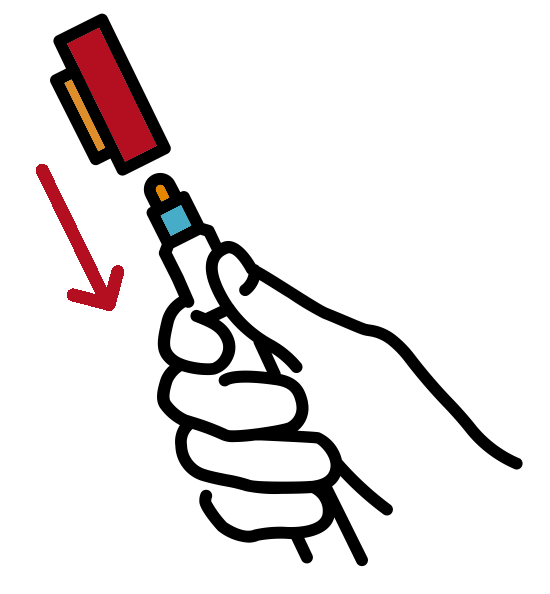
\includegraphics[width=0.2\textwidth,height=\textheight]{figures/recap.png}

}

\end{figure}

Throughout this practical we have covered the topics:

\begin{itemize}
\tightlist
\item
  Linux

  \begin{itemize}
  \tightlist
  \item
    Multiuser Multitasking OS
  \item
    User, Shell and Kernel
  \end{itemize}
\item
  Running commands on the command line

  \begin{itemize}
  \tightlist
  \item
    Search engines, cheat sheets and manual pages
  \item
    Commands: \texttt{man}
  \end{itemize}
\item
  Useful Linux practice and commands

  \begin{itemize}
  \tightlist
  \item
    Tab complete
  \item
    Up and Down arrow keys to access history
  \item
    \textbf{`Ctrl' + `c'} to stop a command
  \item
    Commands: \texttt{clear}
  \end{itemize}
\item
  Files and Directories

  \begin{itemize}
  \tightlist
  \item
    Navigating through directory structure and looking at files with
    paths
  \item
    Commands: \texttt{cd}, \texttt{pwd}, \texttt{ls}, \texttt{mkdir}
  \end{itemize}
\item
  Manipulating files i.e.~creating, copying, moving, deleting

  \begin{itemize}
  \tightlist
  \item
    Commands: \texttt{cp}, \texttt{mv}, \texttt{rm}
  \end{itemize}
\item
  Looking at files

  \begin{itemize}
  \tightlist
  \item
    Commands: \texttt{cat}, \texttt{head}, \texttt{tail}, \texttt{less},
    \texttt{wc}, \texttt{grep}
  \end{itemize}
\item
  Text editor

  \begin{itemize}
  \tightlist
  \item
    Commands: \texttt{vim}
  \end{itemize}
\end{itemize}

\textbf{Note}: There is a cheatsheet at the end of this book with these
commands.

\hypertarget{fastq-format}{%
\chapter{Fastq format}\label{fastq-format}}

\begin{figure}

{\centering 
\includegraphics[width=0.2\textwidth,height=\textheight]{figures/files.png}

}

\end{figure}

The next exercise will focus on a set of files including fastq files.

\begin{itemize}
\tightlist
\item
  Fastq files are very commonly used in bioinformatics.
\item
  Fastq files contain DNA or Amino acid sequenceing data.
\item
  Fastq files contain the nucleotide/amino acid content and its
  sequencing quality for sequences.
\item
  Generally these files are separated by sample but not always.
\item
  A fastq file acts as a normal txt file that can be read but is of a
  specific format.
\item
  One fastq file contains many fastq entries, one after the other.
\item
  Each fastq entry contains four lines.

  \begin{itemize}
  \tightlist
  \item
    One fastq entry represents one sequence.
  \end{itemize}
\end{itemize}

The format of one entry is as below:

\textbf{@Sequence 1}\\
\textbf{CTGTTAAATACCGACTTGCGTCAGGTGCGTGAACAACTGGGCCGCTTT}\\
\textbf{+}\\
\textbf{=\textless\textless\textless=\textgreater@@@ACDCBCDAC@BAA@BA@BBCBBDA@BB@\textgreater CD@A@B?B@@}

The lines represent:\\
1. Header for fastq entry known as the fastq header. This always begins
with a `@'.\\
2. Sequence content of sequence\\
3. Quality header. Always begins with a `+'. Sometimes also contains the
same information as fastq header.\\
4. Quality values for each base in the 2nd line. NOTE: `@' can be used
as quality values.

For more information on the fastq format the below resource is good:
https://en.wikipedia.org/wiki/FASTQ\_format

\hypertarget{exercise-2}{%
\chapter{Exercise 2}\label{exercise-2}}

\begin{figure}

{\centering 
\includegraphics[width=0.15\textwidth,height=\textheight]{figures/exercise_2.png}

}

\end{figure}

The directory \textbf{``\textasciitilde/Linux/6\_final\_exercise/''} has
all the files you need. Below is a set of tasks and questions that will
require all the skills you have gained from this practical.

\begin{enumerate}
\def\labelenumi{\arabic{enumi}.}
\tightlist
\item
  See what files are in the directory.\\
\item
  Rename the file ``3-P£\_CACTTCGA\_L001\_R1\_001.fastq'' as
  ``3-P3\_CACTTCGA\_L001\_R1\_001.fastq''.\\
\item
  Make a backup of the files in a directory called \textbf{backup}.\\
\item
  How many reads are in the samples?\\
\item
  Remove the fastq files with no data.
\item
  Update the backup files with the previous change.\\
\item
  Check if the 1st read names match in the paired files.\\
\item
  Check if the last read names match in the paired files.\\
\item
  In file \textbf{``1-P1\_ATGCCTGG\_L001\_R1\_001.fastq''} look for
  sequence headers with the term `psychrobacter'.\\
\item
  In the sample \textbf{1-P1} remove any fastq entries where the term
  `psychrobacter' appears in the fastq header. Do this for the R1 and R2
  files.\\
\item
  Print to screen the fastq header, sequence and quality data for the
  25th sequence in sample \textbf{2-P2} for both the R1 and R2 file. Do
  this with one command for R1 and a separate command for R2.
\end{enumerate}

You can check my solutions in the
\protect\hyperlink{exercise2_answers}{Answers section}. These are not
the definitive solution but only examples of solutions. If your method
works and you understand why then you have done it correctly.

\part{Advanced topics}

\hypertarget{advancedlinux}{%
\chapter{Advanced Linux practice}\label{advancedlinux}}

\begin{figure}

{\centering 
\includegraphics[width=0.2\textwidth,height=\textheight]{figures/linux_intermdiary.png}

}

\end{figure}

We have covered a small amount of Linux coding. This should be
sufficient to carry out our future workshops but if you were to continue
in bioinformatics we would recommend learning more advanced methods.

Below are some short sections to introduce you to some more advanced
linux coding techniques. These give you a quick overview and some
examples. This will hopefully put you in a good position to allow you to
to learn these techniques in more depth outside of this workshop.

The following sections will all be run with the files in the directory
\textbf{``\textasciitilde/Linux/advanced\_practice/''}. Therefore ensure
you are in this directory before running the below examples. This
contains fastq and txt files for 20 samples. Each sample contains a
fastq file and txt file for uncorrected and corrected reads. These fastq
files are single end (i.e.~there is no reverse/R2 reads).

\hypertarget{wildcard-characters}{%
\section{Wildcard characters}\label{wildcard-characters}}

\begin{figure}

{\centering 
\includegraphics[width=0.2\textwidth,height=\textheight]{figures/wildcard.png}

}

\end{figure}

These are characters that can be used to represent a variety of other
characters. This can be useful for deleting many files, searching for
files with specific patterns in their names and more!

Be very careful when using wildcard character with the command
\textbf{rm}.

Three basic and useful wildcards include:

\begin{itemize}
\tightlist
\item
  \texttt{*} - This represents zero or more characters\\
\item
  \texttt{?} - This represents a single character\\
\item
  \texttt{{[}{]}} - This represents a range of characters
\end{itemize}

Below are various examples you can run to show wildcards in action.

List all the files and directories in the working directory

\begin{Shaded}
\begin{Highlighting}[]
\FunctionTok{ls} \PreprocessorTok{*}
\end{Highlighting}
\end{Shaded}

List all files ending in ``.fastq''

\begin{Shaded}
\begin{Highlighting}[]
\FunctionTok{ls} \PreprocessorTok{*}\NormalTok{.fastq}
\end{Highlighting}
\end{Shaded}

List all files ending in ``.txt''

\begin{Shaded}
\begin{Highlighting}[]
\FunctionTok{ls} \PreprocessorTok{*}\NormalTok{.txt}
\end{Highlighting}
\end{Shaded}

List all files with the string ``corrected'' somewhere in the file name

\begin{Shaded}
\begin{Highlighting}[]
\FunctionTok{ls} \PreprocessorTok{*}\NormalTok{corrected}\PreprocessorTok{*}
\end{Highlighting}
\end{Shaded}

List all files with the string ``corrected'' somewhere in the file name
and it ends in ``fastq''

\begin{Shaded}
\begin{Highlighting}[]
\FunctionTok{ls} \PreprocessorTok{*}\NormalTok{corrected}\PreprocessorTok{*}\NormalTok{fastq}
\end{Highlighting}
\end{Shaded}

List all files that begin with ``sample\_2''

\begin{Shaded}
\begin{Highlighting}[]
\FunctionTok{ls}\NormalTok{ sample\_2}\PreprocessorTok{*}
\end{Highlighting}
\end{Shaded}

List all files that begin with ``sample\_2\_''

\begin{Shaded}
\begin{Highlighting}[]
\FunctionTok{ls}\NormalTok{ sample\_2\_}\PreprocessorTok{*}
\end{Highlighting}
\end{Shaded}

List the files that begin with ``sample\_1'' and ends with ``AAAA.txt''.
It may have zero or more characters between these two.

\begin{Shaded}
\begin{Highlighting}[]
\FunctionTok{ls}\NormalTok{ sample\_1\_}\PreprocessorTok{*}\NormalTok{AAAA.txt}
\end{Highlighting}
\end{Shaded}

List the fastq files of samples with a single digit number

\begin{Shaded}
\begin{Highlighting}[]
\FunctionTok{ls}\NormalTok{ sample\_}\PreprocessorTok{?}\NormalTok{\_}\PreprocessorTok{*}\NormalTok{fastq}
\end{Highlighting}
\end{Shaded}

List the txt files of samples with a number in the tens

\begin{Shaded}
\begin{Highlighting}[]
\FunctionTok{ls}\NormalTok{ sample\_1}\PreprocessorTok{?}\NormalTok{\_}\PreprocessorTok{*}\NormalTok{txt}
\end{Highlighting}
\end{Shaded}

List the txt files for samples 3,4,5,6 \& 7 i.e.~3-7

\begin{Shaded}
\begin{Highlighting}[]
\FunctionTok{ls}\NormalTok{ sample\_}\PreprocessorTok{[}\SpecialStringTok{3}\PreprocessorTok{{-}}\SpecialStringTok{7}\PreprocessorTok{]}\NormalTok{\_}\PreprocessorTok{*}\NormalTok{txt}
\end{Highlighting}
\end{Shaded}

List the txt files for the non corrected information of samples with
single digits.

\begin{Shaded}
\begin{Highlighting}[]
\FunctionTok{ls}\NormalTok{ sample\_}\PreprocessorTok{?}\NormalTok{\_}\PreprocessorTok{*[}\SpecialStringTok{ATGC}\PreprocessorTok{]}\NormalTok{.txt}
\end{Highlighting}
\end{Shaded}

List the corrected txt files for samples with numbers divisible by 10.

\begin{Shaded}
\begin{Highlighting}[]
\FunctionTok{ls}\NormalTok{ sample\_}\PreprocessorTok{[}\SpecialStringTok{0}\PreprocessorTok{{-}}\SpecialStringTok{9}\PreprocessorTok{][}\SpecialStringTok{0}\PreprocessorTok{]}\NormalTok{\_}\PreprocessorTok{*}\NormalTok{corrected.txt}
\end{Highlighting}
\end{Shaded}

\hypertarget{redirection}{%
\section{Redirection}\label{redirection}}

\begin{figure}

{\centering 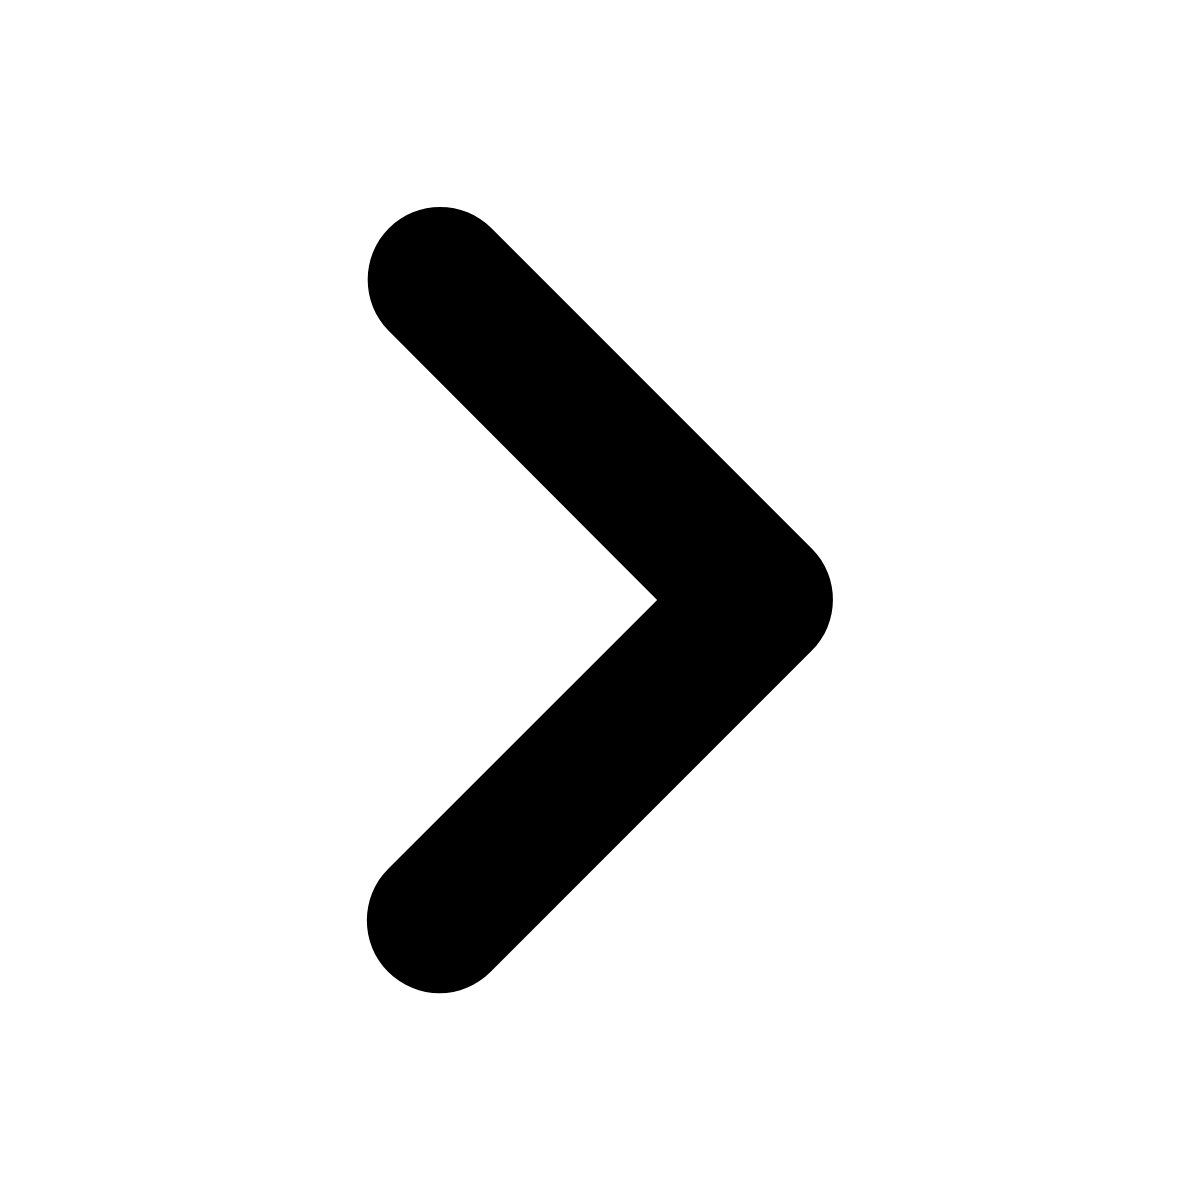
\includegraphics[width=0.15\textwidth,height=\textheight]{figures/chevron.png}

}

\end{figure}

Redirection allows you to put the output of a command to a file. The
redirect symbol is \texttt{\textgreater{}}. Be careful when redirecting
as it will overwrite any existing files. To append to the bottom of a
file use \texttt{\textgreater{}\textgreater{}}.

Below are various examples of redirecting in action.

Create a file called \textbf{ecoli.tmp} containing the text ``I am
escherichia coli''

\begin{Shaded}
\begin{Highlighting}[]
\BuiltInTok{echo}\NormalTok{ “I am escherichia coli” }\OperatorTok{\textgreater{}}\NormalTok{ ecoli.tmp}
\end{Highlighting}
\end{Shaded}

Create a file called \textbf{pcryohalolentis.tmp} containing the text
``I am psychrobacter cryohalolentis''

\begin{Shaded}
\begin{Highlighting}[]
\BuiltInTok{echo}\NormalTok{ “I am psychrobacter cryohaloloentis” }\OperatorTok{\textgreater{}}\NormalTok{ pcryohalolentis.tmp}
\end{Highlighting}
\end{Shaded}

Create a new file called \textbf{bacteria.tmp} which will contain the
text from \textbf{ecoli.tmp} and \textbf{pcryohalolentis.tmp}

\begin{Shaded}
\begin{Highlighting}[]
\FunctionTok{cat} \PreprocessorTok{*}\NormalTok{tmp }\OperatorTok{\textgreater{}}\NormalTok{ bacteria.tmp}
\end{Highlighting}
\end{Shaded}

Create a file called \textbf{vcholerae.tmp} containing the text ``I am
not ecoli or pcryohalolentis''

\begin{Shaded}
\begin{Highlighting}[]
\BuiltInTok{echo}\NormalTok{ “I am not ecoli or pcryohalolentis” }\OperatorTok{\textgreater{}}\NormalTok{ vcholerae.tmp}
\end{Highlighting}
\end{Shaded}

\texttt{cat} the file \textbf{vcholerae.tmp} and redirect it to
\textbf{bacteria.tmp}.

\begin{Shaded}
\begin{Highlighting}[]
\FunctionTok{cat}\NormalTok{ vcholerae.tmp }\OperatorTok{\textgreater{}}\NormalTok{ bacteria.tmp}
\end{Highlighting}
\end{Shaded}

Look at the contents of \textbf{bacteria.tmp}

\begin{Shaded}
\begin{Highlighting}[]
\FunctionTok{cat}\NormalTok{ bacteria.tmp}
\end{Highlighting}
\end{Shaded}

This has removed the ecoli and pcryohalolentis lines. Append the
contents of \textbf{ecoli.tmp} and \textbf{pcryohalolentis.tmp} to
\textbf{bacteria.tmp} and then check the file

\begin{Shaded}
\begin{Highlighting}[]
\FunctionTok{cat}\NormalTok{ ecoli.tmp pcryohalolentis.tmp }\OperatorTok{\textgreater{}\textgreater{}}\NormalTok{ bacteria.tmp}
\FunctionTok{cat}\NormalTok{ bacteria.tmp}
\end{Highlighting}
\end{Shaded}

Put information regarding number of lines of all the fastq files into a
new file called \textbf{fastq\_lines.tmp}

\begin{Shaded}
\begin{Highlighting}[]
\FunctionTok{wc} \AttributeTok{{-}l} \PreprocessorTok{*}\NormalTok{fastq }\OperatorTok{\textgreater{}}\NormalTok{ fastq\_lines.tmp}
\end{Highlighting}
\end{Shaded}

Now delete all the files that were created in the above examples. Again
be very careful about using the \texttt{rm} command with wildcards.

\begin{Shaded}
\begin{Highlighting}[]
\FunctionTok{rm} \PreprocessorTok{*}\NormalTok{tmp}
\end{Highlighting}
\end{Shaded}

\hypertarget{pipes}{%
\section{Pipes}\label{pipes}}

\begin{figure}

{\centering 
\includegraphics[width=0.2\textwidth,height=\textheight]{figures/pipes.png}

}

\end{figure}

Pipes allow you to put the output of one command to the input of
another. For example you could use \texttt{grep} to get all the lines
with a certain string and pipe the output to \texttt{wc} to count the
number of lines that have the specific string.

The pipe symbol is \texttt{\textbar{}}. This is normally found on your
keyboard directly left of the Z key. Weirdly the symbol is represented
by \texttt{\textbar{}} but split in the middle on some keyboards.

A useful tip when building up longer pipes is to start with a smaller
amount of data and check the output of each step as you go. To do this
you could use \texttt{head} instead of \texttt{cat} whilst testing.

Below are various examples of piping in action

Print to screen the second last fastq entry of the file
\textbf{sample\_20\_ATAC\_corrected.fastq}

\begin{Shaded}
\begin{Highlighting}[]
\FunctionTok{cat}\NormalTok{ sample\_20\_ATAC\_corrected.fastq }\KeywordTok{|} \FunctionTok{tail} \AttributeTok{{-}n}\NormalTok{ 8 }\KeywordTok{|} \FunctionTok{head} \AttributeTok{{-}n}\NormalTok{ 4 }
\end{Highlighting}
\end{Shaded}

\textbf{Note}: In the above command the \texttt{tail} command is working
on the output of the \texttt{cat} command. Therefore this would not work
to get the second last fastq entry of multiple files. For example the
following command would print the second last fastq entry of the last
fastq file (i.e.~\textbf{sample\_9\_AAGA.fastq} due to file ordering)

\begin{Shaded}
\begin{Highlighting}[]
\FunctionTok{cat} \PreprocessorTok{*}\NormalTok{fastq }\KeywordTok{|} \FunctionTok{tail} \AttributeTok{{-}n}\NormalTok{ 8 }\KeywordTok{|} \FunctionTok{head} \AttributeTok{{-}n}\NormalTok{ 4}
\end{Highlighting}
\end{Shaded}

Count the number of lines within all the fastq files

\begin{Shaded}
\begin{Highlighting}[]
\FunctionTok{cat} \PreprocessorTok{*}\NormalTok{fastq }\KeywordTok{|} \FunctionTok{wc} \AttributeTok{{-}l}
\end{Highlighting}
\end{Shaded}

Count the number of lines which contain the text ``TAG'' within all the
fastq files

\begin{Shaded}
\begin{Highlighting}[]
\FunctionTok{cat} \PreprocessorTok{*}\NormalTok{fastq }\KeywordTok{|} \FunctionTok{grep}\NormalTok{ “TAG” }\KeywordTok{|} \FunctionTok{wc} \AttributeTok{{-}l}
\end{Highlighting}
\end{Shaded}

\hypertarget{regular-expressions}{%
\section{Regular expressions}\label{regular-expressions}}

\begin{figure}

{\centering \includegraphics[width=0.2\textwidth,height=\textheight]{figures/trex.png}

}

\end{figure}

Regular expressions are similar to wildcard characters but more complex
and used for commands like \texttt{grep} and \texttt{sed}.

Below are a basic set of regular expressions:

\begin{itemize}
\tightlist
\item
  \texttt{.} : A single character\\
\item
  \texttt{?} : The preceding character matches 1 or 0 times\\
\item
  \texttt{*} : The preceding character matches zero or more times\\
\item
  \texttt{+} : The preceding character matches one or more times\\
\item
  \texttt{\{n\}} : The preceding character matches exactly n times\\
\item
  \texttt{\{n,m\}} : The preceding character matches n to m times\\
\item
  \texttt{{[}AT{]}} : The character is one of the characters in the
  brackets\\
\item
  \texttt{{[}\^{}CG{]}} : The character is not one of those in the
  brackets\\
\item
  \texttt{{[}1-7{]}} : The character is 1,2,3,4,5,6 or 7. This works
  with letters too.\\
\item
  \texttt{()} : Group several characters into one\\
\item
  \texttt{\textbar{}} : Logical OR operator\\
\item
  \texttt{\^{}} : Matches the beginning of the line\\
\item
  \texttt{\$} : Matches the end of the line
\end{itemize}

Below are various examples of regular expressions in action.

Look at the contents of \textbf{metadata.txt}

\begin{Shaded}
\begin{Highlighting}[]
\FunctionTok{cat}\NormalTok{ metadata.txt}
\end{Highlighting}
\end{Shaded}

!Print out the lines for the Healthy patients

\begin{Shaded}
\begin{Highlighting}[]
\FunctionTok{cat}\NormalTok{ metadata.txt }\KeywordTok{|} \FunctionTok{grep}\NormalTok{ “HEALTHY”}
\end{Highlighting}
\end{Shaded}

Print out the lines for the IBD patients from Craigavon and Belfast. In
the below command \texttt{\textbackslash{}} is used to allow
\texttt{\textbar{}} to be used as an \textbf{or} operator instead of
acting as a string to match.

\begin{Shaded}
\begin{Highlighting}[]
\FunctionTok{cat}\NormalTok{ metadata.txt }\KeywordTok{|} \FunctionTok{grep} \StringTok{"IBD"} \KeywordTok{|} \FunctionTok{grep} \StringTok{"BELFAST\textbackslash{}|CRAIGAVON"}
\end{Highlighting}
\end{Shaded}

Print out the lines for the Pre information of patients not from
Edinburgh or Aberdeen

\begin{Shaded}
\begin{Highlighting}[]
\FunctionTok{cat}\NormalTok{ metadata.txt }\KeywordTok{|} \FunctionTok{grep} \StringTok{"PRE$"} \KeywordTok{|} \FunctionTok{grep} \AttributeTok{{-}v} \StringTok{"ABERDEEN\textbackslash{}|EDINBURGH"}
\end{Highlighting}
\end{Shaded}

Print out the lines for patients 1,2,3 and 4

\begin{Shaded}
\begin{Highlighting}[]
\FunctionTok{cat}\NormalTok{ metadata.txt }\KeywordTok{|} \FunctionTok{grep} \StringTok{"Patient\_[1{-}4][\^{}0{-}9]"} 
\end{Highlighting}
\end{Shaded}

Print to screen every fastq header of file
\textbf{sample\_15\_AACG\_corrected.fastq}

\begin{Shaded}
\begin{Highlighting}[]
\FunctionTok{cat}\NormalTok{ sample\_15\_AACG\_corrected.fastq }\KeywordTok{|} \FunctionTok{grep}\NormalTok{ “\^{}@sample”}
\end{Highlighting}
\end{Shaded}

In the piping examples we counted the number of lines with the text
``TAG'' within the fastq files. However this also counted fastq headers
due to the name of the samples. Let us use a regular expression to only
count the number of sequences within the fastq files that contain
``TAG''.

\begin{Shaded}
\begin{Highlighting}[]
\FunctionTok{cat} \PreprocessorTok{*}\NormalTok{fastq }\KeywordTok{|} \FunctionTok{grep}\NormalTok{ “\^{}}\PreprocessorTok{[\^{}}\SpecialStringTok{@}\PreprocessorTok{]}\NormalTok{.}\PreprocessorTok{*}\NormalTok{TAG”}
\end{Highlighting}
\end{Shaded}

Print to screen every line within the file
\textbf{sample\_3\_AAAG\_corrected.fastq} that has a possible Threonine
codon in the forward direction.

\begin{Shaded}
\begin{Highlighting}[]
\FunctionTok{grep} \StringTok{"\^{}[\^{}@].*AC[ACTG]"}\NormalTok{ sample\_3\_AAAG\_corrected.fastq}
\end{Highlighting}
\end{Shaded}

In the above example fastq quality lines are also extracted as some of
them also contain the pattern we are searching for. To get around this
we can pipe. First grep the fastq quality header (i.e.~+), as no other
line only contains ``+'', and the line before it. Then we can remove
lines with only a plus with an invert grep. Finally we can grep for the
threonine pattern using only the sequence lines. Let us build this up
step by step.

Print to screen the fastq quality header plus the one line preceding
each (i.e.~Sequence line) for file
\textbf{sample\_3\_AAAG\_corrected.fastq.}

\begin{Shaded}
\begin{Highlighting}[]
\FunctionTok{grep} \AttributeTok{{-}B}\NormalTok{ 1 “\^{}+$” sample\_3\_AAAG\_corrected.fastq}
\end{Highlighting}
\end{Shaded}

Now pipe this output so it removes the lines with ``+'' (fastq quality
headers) and ``--'' (separators of each \texttt{grep} match provided by
grep because of the -B 1 option).

\begin{Shaded}
\begin{Highlighting}[]
\FunctionTok{grep} \AttributeTok{{-}B}\NormalTok{ 1 }\StringTok{"\^{}+$"}\NormalTok{ sample\_3\_AAAG\_corrected.fastq }\KeywordTok{|} \FunctionTok{grep} \AttributeTok{{-}v} \StringTok{"+\textbackslash{}|{-}{-}"}
\end{Highlighting}
\end{Shaded}

Now from this output, \texttt{grep} for the Threonine pattern plus
colour each match within the line with the option ``\textbf{--color}''.

\begin{Shaded}
\begin{Highlighting}[]
\FunctionTok{grep} \AttributeTok{{-}B}\NormalTok{ 1 }\StringTok{"\^{}+$"}\NormalTok{ sample\_3\_AAAG\_corrected.fastq }\KeywordTok{|} \FunctionTok{grep} \AttributeTok{{-}v} \StringTok{"+\textbackslash{}|{-}{-}"} \KeywordTok{|} \FunctionTok{grep} \AttributeTok{{-}{-}color} \StringTok{"AC[ACTG]"}
\end{Highlighting}
\end{Shaded}

Let us repeat the above but add the possibility of the threonine being
in the reverse direction.

\begin{Shaded}
\begin{Highlighting}[]
\FunctionTok{grep} \AttributeTok{{-}B}\NormalTok{ 1 }\StringTok{"\^{}+$"}\NormalTok{ sample\_3\_AAAG\_corrected.fastq }\KeywordTok{|} \FunctionTok{grep} \AttributeTok{{-}v} \StringTok{"+\textbackslash{}|{-}{-}"} \DataTypeTok{\textbackslash{}}
\KeywordTok{|} \FunctionTok{grep} \AttributeTok{{-}{-}color} \StringTok{"AC[ACTG]\textbackslash{}|[ACTG]CA"}
\end{Highlighting}
\end{Shaded}

\textbf{Resources to learn more in the future}

Rex Egg, A good resource to learn more about regular expressions:

https://www.rexegg.com/

Cheatsheet:

https://www.rexegg.com/regex-quickstart.html

Regex Crossword, A online game like soduku that is useful to practice
regular expressions. Best used in conjunction with the above cheat
sheet:

https://regexcrossword.com/

\hypertarget{sed}{%
\section{sed}\label{sed}}

\begin{figure}

{\centering \includegraphics[width=0.2\textwidth,height=\textheight]{figures/sed.png}

}

\end{figure}

This is a complicated yet powerful command that can be used to edit text
files quickly and efficiently. The main use is to substitute text with
other text. \texttt{sed} can be used with regular expressions.

The basic outline of a \texttt{sed} substitute command is as below. In
the below case \texttt{s/} signifies that \texttt{sed} will be used for
substitution

\begin{Shaded}
\begin{Highlighting}[]
\FunctionTok{sed}\NormalTok{ “s/old\_text/new\_text/” old\_file }\OperatorTok{\textgreater{}}\NormalTok{ new\_file}
\end{Highlighting}
\end{Shaded}

Below are some examples of sed in action.

Print out a list of all the sample names using the fastq files

\begin{Shaded}
\begin{Highlighting}[]
\FunctionTok{ls} \AttributeTok{{-}1} \PreprocessorTok{*[}\SpecialStringTok{AGTC}\PreprocessorTok{]}\NormalTok{.fastq }\KeywordTok{|} \FunctionTok{sed} \StringTok{"s/.fastq//"}
\end{Highlighting}
\end{Shaded}

First print out the contents of the file \textbf{metadata.txt}

\begin{Shaded}
\begin{Highlighting}[]
\FunctionTok{cat}\NormalTok{ metadata.txt}
\end{Highlighting}
\end{Shaded}

Print out \textbf{metadata.txt} and change IBD to DISEASE without
altering the file

\begin{Shaded}
\begin{Highlighting}[]
\FunctionTok{sed} \StringTok{"s/IBD/DISEASE/"}\NormalTok{ metadata.txt}
\end{Highlighting}
\end{Shaded}

or

\begin{Shaded}
\begin{Highlighting}[]
\FunctionTok{cat}\NormalTok{ metadata.txt }\KeywordTok{|} \FunctionTok{sed} \StringTok{"s/IBD/DISEASE/"}
\end{Highlighting}
\end{Shaded}

\texttt{sed} is case sensitive and will by default only replace the
first instance it finds within each line. Print \textbf{metadata.txt} to
screen and then change the ``P'' in ``Patient'' to ``Human\_P''

\begin{Shaded}
\begin{Highlighting}[]
\FunctionTok{cat}\NormalTok{ metadata.txt }\KeywordTok{|} \FunctionTok{sed} \StringTok{"s/P/Human\_P/"}
\end{Highlighting}
\end{Shaded}

To replace every instance of the old pattern within each line \texttt{g}
can be added after the last \texttt{/}. This stands for global therefore
it changes the command to a global substitute.

Print \textbf{metadata.txt} to screen and change every occurrence of a
number to ``number''. To get the regular expression meaning of ``+'' it
needs a ``\textbf{\texttt{\textbackslash{}}}'' before the ``+''

\begin{Shaded}
\begin{Highlighting}[]
\FunctionTok{cat}\NormalTok{ metadata.txt }\KeywordTok{|} \FunctionTok{sed} \StringTok{"s/[0{-}9]\textbackslash{}+/number/g"}
\end{Highlighting}
\end{Shaded}

The file metadata.txt is tab delimited (i.e.~there is a tab between each
column. Make a comma separated file containing the information of
\textbf{metadata.txt} called \textbf{metadata.csv} (csv = comma
separated value). \texttt{\textbackslash{}t} presents a tab.

\begin{Shaded}
\begin{Highlighting}[]
\FunctionTok{cat}\NormalTok{ metadata.txt }\KeywordTok{|} \FunctionTok{sed} \StringTok{"s/\textbackslash{}t/,/g"} \OperatorTok{\textgreater{}}\NormalTok{ metadata.csv}
\end{Highlighting}
\end{Shaded}

For a very in depth look into the sed command please look at the
following link: http://www.grymoire.com/Unix/Sed.html

\hypertarget{permissions}{%
\section{Permissions}\label{permissions}}

All files, directories and programs have permissions. It is important to
know about this so you know your read, write and executability
permissions for the content within machines.

Below is a useful link to learn about file permissions:\\
https://www.guru99.com/file-permissions.html

\hypertarget{mcqs-advanced-linux}{%
\section{MCQs: Advanced linux}\label{mcqs-advanced-linux}}

\begin{figure}

{\centering \includegraphics[width=0.2\textwidth,height=\textheight]{figures/question_bubble_red.png}

}

\end{figure}

Please attempt to answer the below Multiple-Choice Questions to
reinforce what you have learnt in this chapter.

\begin{enumerate}
\def\labelenumi{\arabic{enumi}.}
\tightlist
\item
  Which symbol is used to pipe the output of one command to the input of
  another?
\end{enumerate}

\begin{itemize}
\item
  \begin{enumerate}
  \def\labelenumi{(\Alph{enumi})}
  \tightlist
  \item
    \textbf{\texttt{\textgreater{}}}\strut \\
  \end{enumerate}
\item
  \begin{enumerate}
  \def\labelenumi{(\Alph{enumi})}
  \setcounter{enumi}{1}
  \tightlist
  \item
    \textbf{\texttt{\textbar{}}}\strut \\
  \end{enumerate}
\item
  \begin{enumerate}
  \def\labelenumi{(\Alph{enumi})}
  \setcounter{enumi}{2}
  \tightlist
  \item
    \textbf{\texttt{sed}}
  \end{enumerate}
\end{itemize}

\begin{enumerate}
\def\labelenumi{\arabic{enumi}.}
\setcounter{enumi}{1}
\tightlist
\item
  What command can be used to substitute text with other text?
\end{enumerate}

\begin{itemize}
\item
  \begin{enumerate}
  \def\labelenumi{(\Alph{enumi})}
  \tightlist
  \item
    \textbf{\texttt{\textgreater{}}}\strut \\
  \end{enumerate}
\item
  \begin{enumerate}
  \def\labelenumi{(\Alph{enumi})}
  \setcounter{enumi}{1}
  \tightlist
  \item
    \textbf{\texttt{\textbar{}}}\strut \\
  \end{enumerate}
\item
  \begin{enumerate}
  \def\labelenumi{(\Alph{enumi})}
  \setcounter{enumi}{2}
  \tightlist
  \item
    \textbf{\texttt{sed}}
  \end{enumerate}
\end{itemize}

\begin{enumerate}
\def\labelenumi{\arabic{enumi}.}
\setcounter{enumi}{2}
\tightlist
\item
  Which symbol is used to redirect the output of a command to a file?
\end{enumerate}

\begin{itemize}
\item
  \begin{enumerate}
  \def\labelenumi{(\Alph{enumi})}
  \tightlist
  \item
    \textbf{\texttt{\textgreater{}}}\strut \\
  \end{enumerate}
\item
  \begin{enumerate}
  \def\labelenumi{(\Alph{enumi})}
  \setcounter{enumi}{1}
  \tightlist
  \item
    \textbf{\texttt{\textbar{}}}\strut \\
  \end{enumerate}
\item
  \begin{enumerate}
  \def\labelenumi{(\Alph{enumi})}
  \setcounter{enumi}{2}
  \tightlist
  \item
    \textbf{\texttt{sed}}
  \end{enumerate}
\end{itemize}

\begin{enumerate}
\def\labelenumi{\arabic{enumi}.}
\setcounter{enumi}{3}
\tightlist
\item
  Which wildcard represents a single character?
\end{enumerate}

\begin{itemize}
\item
  \begin{enumerate}
  \def\labelenumi{(\Alph{enumi})}
  \tightlist
  \item
    \textbf{\texttt{*}}\strut \\
  \end{enumerate}
\item
  \begin{enumerate}
  \def\labelenumi{(\Alph{enumi})}
  \setcounter{enumi}{1}
  \tightlist
  \item
    \textbf{\texttt{{[}{]}}}\strut \\
  \end{enumerate}
\item
  \begin{enumerate}
  \def\labelenumi{(\Alph{enumi})}
  \setcounter{enumi}{2}
  \tightlist
  \item
    \textbf{\texttt{?}}
  \end{enumerate}
\end{itemize}

\begin{enumerate}
\def\labelenumi{\arabic{enumi}.}
\setcounter{enumi}{4}
\tightlist
\item
  Which wildcard represents zero or more characters?
\end{enumerate}

\begin{itemize}
\item
  \begin{enumerate}
  \def\labelenumi{(\Alph{enumi})}
  \tightlist
  \item
    \textbf{\texttt{*}}\strut \\
  \end{enumerate}
\item
  \begin{enumerate}
  \def\labelenumi{(\Alph{enumi})}
  \setcounter{enumi}{1}
  \tightlist
  \item
    \textbf{\texttt{{[}{]}}}\strut \\
  \end{enumerate}
\item
  \begin{enumerate}
  \def\labelenumi{(\Alph{enumi})}
  \setcounter{enumi}{2}
  \tightlist
  \item
    \textbf{\texttt{?}}
  \end{enumerate}
\end{itemize}

\begin{enumerate}
\def\labelenumi{\arabic{enumi}.}
\setcounter{enumi}{5}
\tightlist
\item
  Which wildcard represents a range of characters?
\end{enumerate}

\begin{itemize}
\item
  \begin{enumerate}
  \def\labelenumi{(\Alph{enumi})}
  \tightlist
  \item
    \textbf{\texttt{*}}\strut \\
  \end{enumerate}
\item
  \begin{enumerate}
  \def\labelenumi{(\Alph{enumi})}
  \setcounter{enumi}{1}
  \tightlist
  \item
    \textbf{\texttt{{[}{]}}}\strut \\
  \end{enumerate}
\item
  \begin{enumerate}
  \def\labelenumi{(\Alph{enumi})}
  \setcounter{enumi}{2}
  \tightlist
  \item
    \textbf{\texttt{?}}
  \end{enumerate}
\end{itemize}

\begin{enumerate}
\def\labelenumi{\arabic{enumi}.}
\setcounter{enumi}{6}
\tightlist
\item
  Which regular expression indicates that the preceding character
  matches 1 or 0 times?
\end{enumerate}

\begin{itemize}
\item
  \begin{enumerate}
  \def\labelenumi{(\Alph{enumi})}
  \tightlist
  \item
    \textbf{\texttt{.}}\strut \\
  \end{enumerate}
\item
  \begin{enumerate}
  \def\labelenumi{(\Alph{enumi})}
  \setcounter{enumi}{1}
  \tightlist
  \item
    \textbf{\texttt{?}}\strut \\
  \end{enumerate}
\item
  \begin{enumerate}
  \def\labelenumi{(\Alph{enumi})}
  \setcounter{enumi}{2}
  \tightlist
  \item
    \textbf{\texttt{*}}
  \end{enumerate}
\end{itemize}

\begin{enumerate}
\def\labelenumi{\arabic{enumi}.}
\setcounter{enumi}{7}
\tightlist
\item
  Which regular expression represents a single character?
\end{enumerate}

\begin{itemize}
\item
  \begin{enumerate}
  \def\labelenumi{(\Alph{enumi})}
  \tightlist
  \item
    \textbf{\texttt{.}}\strut \\
  \end{enumerate}
\item
  \begin{enumerate}
  \def\labelenumi{(\Alph{enumi})}
  \setcounter{enumi}{1}
  \tightlist
  \item
    \textbf{\texttt{?}}\strut \\
  \end{enumerate}
\item
  \begin{enumerate}
  \def\labelenumi{(\Alph{enumi})}
  \setcounter{enumi}{2}
  \tightlist
  \item
    \textbf{\texttt{*}}
  \end{enumerate}
\end{itemize}

\begin{enumerate}
\def\labelenumi{\arabic{enumi}.}
\setcounter{enumi}{8}
\tightlist
\item
  Which regular expression indicates that the preceding character
  matches zero or more times?
\end{enumerate}

\begin{itemize}
\item
  \begin{enumerate}
  \def\labelenumi{(\Alph{enumi})}
  \tightlist
  \item
    \textbf{\texttt{.}}\strut \\
  \end{enumerate}
\item
  \begin{enumerate}
  \def\labelenumi{(\Alph{enumi})}
  \setcounter{enumi}{1}
  \tightlist
  \item
    \textbf{\texttt{?}}\strut \\
  \end{enumerate}
\item
  \begin{enumerate}
  \def\labelenumi{(\Alph{enumi})}
  \setcounter{enumi}{2}
  \tightlist
  \item
    \textbf{\texttt{*}}
  \end{enumerate}
\end{itemize}

\begin{enumerate}
\def\labelenumi{\arabic{enumi}.}
\setcounter{enumi}{9}
\tightlist
\item
  Which regular expression matches the end of the line?
\end{enumerate}

\begin{itemize}
\item
  \begin{enumerate}
  \def\labelenumi{(\Alph{enumi})}
  \tightlist
  \item
    \textbf{\texttt{\textbar{}}}\strut \\
  \end{enumerate}
\item
  \begin{enumerate}
  \def\labelenumi{(\Alph{enumi})}
  \setcounter{enumi}{1}
  \tightlist
  \item
    \textbf{\texttt{\^{}}}\strut \\
  \end{enumerate}
\item
  \begin{enumerate}
  \def\labelenumi{(\Alph{enumi})}
  \setcounter{enumi}{2}
  \tightlist
  \item
    \textbf{\texttt{\$}}
  \end{enumerate}
\end{itemize}

\begin{enumerate}
\def\labelenumi{\arabic{enumi}.}
\setcounter{enumi}{10}
\tightlist
\item
  Which regular expression is a logical OR operator?
\end{enumerate}

\begin{itemize}
\item
  \begin{enumerate}
  \def\labelenumi{(\Alph{enumi})}
  \tightlist
  \item
    \textbf{\texttt{\textbar{}}}\strut \\
  \end{enumerate}
\item
  \begin{enumerate}
  \def\labelenumi{(\Alph{enumi})}
  \setcounter{enumi}{1}
  \tightlist
  \item
    \textbf{\texttt{\^{}}}\strut \\
  \end{enumerate}
\item
  \begin{enumerate}
  \def\labelenumi{(\Alph{enumi})}
  \setcounter{enumi}{2}
  \tightlist
  \item
    \textbf{\texttt{\$}}
  \end{enumerate}
\end{itemize}

\begin{enumerate}
\def\labelenumi{\arabic{enumi}.}
\setcounter{enumi}{11}
\tightlist
\item
  Which regular expression matches the start of the line?
\end{enumerate}

\begin{itemize}
\item
  \begin{enumerate}
  \def\labelenumi{(\Alph{enumi})}
  \tightlist
  \item
    \textbf{\texttt{\textbar{}}}\strut \\
  \end{enumerate}
\item
  \begin{enumerate}
  \def\labelenumi{(\Alph{enumi})}
  \setcounter{enumi}{1}
  \tightlist
  \item
    \textbf{\texttt{\^{}}}\strut \\
  \end{enumerate}
\item
  \begin{enumerate}
  \def\labelenumi{(\Alph{enumi})}
  \setcounter{enumi}{2}
  \tightlist
  \item
    \textbf{\texttt{\$}}
  \end{enumerate}
\end{itemize}

\hypertarget{advance-practice-exercise}{%
\chapter{Advance practice exercise}\label{advance-practice-exercise}}

\begin{figure}

{\centering \includegraphics[width=0.2\textwidth,height=\textheight]{figures/adv_exercise.png}

}

\end{figure}

\begin{enumerate}
\def\labelenumi{\arabic{enumi}.}
\tightlist
\item
  Copy the directory \textbf{\textasciitilde/Linux/advanced\_practice}
  to \textbf{\textasciitilde/Linux/advanced\_practice\_exercise}
\item
  Move into \textbf{\textasciitilde/Linux/advanced\_practice\_exercise}
\item
  Make a directory called \textbf{fastq} and one called \textbf{txt}
\item
  With one command move all the fastq files into the directory
  \textbf{fastq}
\item
  With one command move all the txt files, excluding
  \textbf{metadata.txt} and \textbf{samples.txt}, into the directory
  \textbf{txt}
\item
  Create a file in the \textbf{fastq} directory called
  \textbf{patient\_1\_corrected.fastq} and put all the corrected fastq
  data for patient\_1 into the file. You can look at the metadat.txt
  file to see which samples belong to patient\_1.
\item
  Append the metadata line for sample\_1\_AAAA to the bottom of the file
  \textbf{sample\_1\_AAAA.txt} in the \textbf{txt} directory.
\item
  For all the corrected fastq files find the sequences that start with a
  stop codon in the forward orientation (i.e.~TAG, TAA or TGA). Print
  out to screen the sample name and sequence info separated by a ``:''
  only
  (e.g.~sample\_10\_AAGT:TAAGAGAACAATGAACAGATATTAATAATTTTGCCGCTTTTCTGCGGGAT)
\item
  Count the number of Gs and Cs within file
  \textbf{sample\_16\_AACC.fastq}
\item
  Get the fastq headers of sequences with homopolymers made of As with a
  length of 5 or greater for the uncorrected fastq files for samples
  3,4,5,13,14 and 15 with one command.
\end{enumerate}

You can check my solutions in the
\protect\hyperlink{exerciseadv_answers}{Answers section}. These are not
the definitive solution but only examples of solutions. If your method
works and you understand why then you have done it correctly.

\hypertarget{bfxlanguages}{%
\chapter{Bioinformatic Languages}\label{bfxlanguages}}

\begin{figure}

{\centering \includegraphics[width=0.2\textwidth,height=\textheight]{figures/languages.png}

}

\end{figure}

Unfortunately you cannot do everything you would want directly on the
Linux command line. Even the tasks you can do are sometimes not very
efficient or easy. Fortunately there are many other programming
languages you can use. There is a large amount of other programming
languages and it can be hard to know which one to learn. Below is a list
of commonly used bioinformatic program languages with a brief summary on
their purpose and links to online resources to introduce you to the
language.

\hypertarget{awk}{%
\section{awk}\label{awk}}

\texttt{awk} is typically used as a data extraction and reporting tool.
It is very good due to its power and versatility.

Tutorial:

http://www.grymoire.com/Unix/Awk.html

Manual:

https://www.gnu.org/software/gawk/manual/gawk.html

\hypertarget{python}{%
\section{Python}\label{python}}

\begin{figure}

{\centering \includegraphics[width=0.2\textwidth,height=\textheight]{figures/python.png}

}

\end{figure}

Python is used for software development and other applications It is
favoured in Bioinformatics due to its relative ease to learn and it is
able to handle strings well (i.e.~genetic code). There are also many
packages for python that help the analysis of biological data and other
scientific data.

Python website:

https://www.python.org/

BioPython:

https://biopython.org/

\hypertarget{perl}{%
\section{Perl}\label{perl}}

\begin{figure}

{\centering \includegraphics[width=0.2\textwidth,height=\textheight]{figures/perl.png}

}

\end{figure}

Perl is a similar language to python with similar uses. The main
difference is how they look.

Tutorial:

https://www.tutorialspoint.com/perl/perl\_introduction.htm

Perl website:

https://www.perl.org/

BioPerl:

https://bioperl.org/

\hypertarget{python-or-perl}{%
\section{Python or Perl?}\label{python-or-perl}}

Generally speaking people normally choose to either learn python or
perl. However there are many bioinformatic tools written in perl and
many written in python. Therefore it is good to know a bit in both so
you can debug scripts and specialise in one so you can write your own
scripts. Our suggestion would be to specialise in Python due to its ease
to learn and its growing popularity in the Bioinformatics field. However
there are also other upcoming programming languages that are becoming
more popular in bioinformatics, so you may like to give them a look.

\hypertarget{ruby}{%
\section{Ruby}\label{ruby}}

\begin{figure}

{\centering \includegraphics[width=0.2\textwidth,height=\textheight]{figures/ruby.png}

}

\end{figure}

A programming language that is becoming more popular in bioinformatics
due to its beginner friendliness.

Tutorial:

http://rubylearning.com/

Ruby website:

https://www.ruby-lang.org/en/

BioRuby:

http://bioruby.org/

Why learn Ruby?

http://www.bestprogramminglanguagefor.me/why-learn-ruby

\hypertarget{golang-aka-go}{%
\section{Golang (AKA Go)}\label{golang-aka-go}}

\begin{figure}

{\centering \includegraphics[width=0.2\textwidth,height=\textheight]{figures/golang.png}

}

\end{figure}

Another easy programming language with a library specifically made for
bioinformatics.

Tutorial:

https://tour.golang.org/welcome/1

Go website:

https://golang.org/

biogo:

https://github.com/biogo/biogo

\hypertarget{r}{%
\section{R}\label{r}}

\begin{figure}

{\centering \includegraphics[width=0.2\textwidth,height=\textheight]{figures/R.png}

}

\end{figure}

R is a very powerful programming language for statistical analysis and
visualisation. It unfortunately has a large barrier to entry and
normally quite unclear documentation. However it will unlikely be
surpassed by another language any time soon due to its widespread use
and large amount of very useful and powerful packages for various uses
in the public domain. We would recommend using the IDE Rstudio when
using R.

Tutorial:

https://swirlstats.com/

R Website:

https://www.r-project.org/

Cran Website:

https://cran.r-project.org/

Rstudio Website:

https://www.rstudio.com/

\part{Answers}

\hypertarget{exercise1_answers}{%
\chapter*{Exercise 1}\label{exercise1_answers}}
\addcontentsline{toc}{chapter}{Exercise 1}

\markboth{Exercise 1}{Exercise 1}

\begin{figure}

{\centering \includegraphics[width=0.2\textwidth,height=\textheight]{figures/exercise.png}

}

\end{figure}

Ensure you are in the correct directory before carrying out the below
commands

\begin{Shaded}
\begin{Highlighting}[]
\BuiltInTok{cd}\NormalTok{ \textasciitilde{}/Linux/}
\end{Highlighting}
\end{Shaded}

\begin{enumerate}
\def\labelenumi{\arabic{enumi}.}
\tightlist
\item
  Change the name of the subdirectory 4\_exercises\_aaaa within your
  Linux to 4\_exercises
\end{enumerate}

\begin{Shaded}
\begin{Highlighting}[]
\FunctionTok{mv}\NormalTok{ 4\_exercises\_aaaa 4\_exercises}
\end{Highlighting}
\end{Shaded}

\begin{enumerate}
\def\labelenumi{\arabic{enumi}.}
\setcounter{enumi}{1}
\tightlist
\item
  Make a backup of the 4\_exercises directory
\end{enumerate}

\begin{Shaded}
\begin{Highlighting}[]
\FunctionTok{cp} \AttributeTok{{-}r}\NormalTok{ 4\_exercises 4\_exercises\_backup }
\end{Highlighting}
\end{Shaded}

\begin{enumerate}
\def\labelenumi{\arabic{enumi}.}
\setcounter{enumi}{2}
\tightlist
\item
  List the contents of the 4\_exercises directory
\end{enumerate}

\begin{Shaded}
\begin{Highlighting}[]
\FunctionTok{ls}\NormalTok{ 4\_exercises}
\end{Highlighting}
\end{Shaded}

\begin{enumerate}
\def\labelenumi{\arabic{enumi}.}
\setcounter{enumi}{3}
\tightlist
\item
  Within the directory 4\_exercises
\end{enumerate}

\begin{Shaded}
\begin{Highlighting}[]
\BuiltInTok{cd}\NormalTok{ 4\_exercises}
\end{Highlighting}
\end{Shaded}

Print the working directory

\begin{Shaded}
\begin{Highlighting}[]
\BuiltInTok{pwd}
\end{Highlighting}
\end{Shaded}

\begin{enumerate}
\def\labelenumi{\alph{enumi}.}
\setcounter{enumi}{1}
\tightlist
\item
  Print out to screen the phrase `the echo command allows me to print
  phrases to screen'
\end{enumerate}

\begin{Shaded}
\begin{Highlighting}[]
\BuiltInTok{echo}\NormalTok{ “the echo command allows me to print phrases to screen”}
\end{Highlighting}
\end{Shaded}

\begin{enumerate}
\def\labelenumi{\alph{enumi}.}
\setcounter{enumi}{2}
\tightlist
\item
  Copy the file copy\_this\_file.txt to the directory to\_me
\end{enumerate}

\begin{Shaded}
\begin{Highlighting}[]
\FunctionTok{cp}\NormalTok{ copy\_this\_file.txt to\_me}
\end{Highlighting}
\end{Shaded}

\begin{enumerate}
\def\labelenumi{\alph{enumi}.}
\setcounter{enumi}{3}
\tightlist
\item
  Rename the directory to\_me to you
\end{enumerate}

\begin{Shaded}
\begin{Highlighting}[]
\FunctionTok{mv}\NormalTok{ to\_me you}
\end{Highlighting}
\end{Shaded}

\begin{enumerate}
\def\labelenumi{\alph{enumi}.}
\setcounter{enumi}{5}
\tightlist
\item
  Delete the initial copy\_this\_file.txt file
\end{enumerate}

\begin{Shaded}
\begin{Highlighting}[]
\FunctionTok{rm}\NormalTok{ copy\_this\_file.txt}
\end{Highlighting}
\end{Shaded}

\hypertarget{exercise2_answers}{%
\chapter*{Exercise 2}\label{exercise2_answers}}
\addcontentsline{toc}{chapter}{Exercise 2}

\markboth{Exercise 2}{Exercise 2}

\begin{figure}

{\centering \includegraphics[width=0.2\textwidth,height=\textheight]{figures/exercise_2.png}

}

\end{figure}

Ensure you are in the correct directory before carrying out the below
commands

\begin{Shaded}
\begin{Highlighting}[]
\BuiltInTok{cd}\NormalTok{ \textasciitilde{}/Linux/6\_final\_exercise}
\end{Highlighting}
\end{Shaded}

\begin{enumerate}
\def\labelenumi{\arabic{enumi}.}
\tightlist
\item
  See what files are in the directory
\end{enumerate}

\begin{Shaded}
\begin{Highlighting}[]
\FunctionTok{ls}
\end{Highlighting}
\end{Shaded}

\begin{enumerate}
\def\labelenumi{\arabic{enumi}.}
\setcounter{enumi}{1}
\tightlist
\item
  Rename the file 3-P£\_CACTTCGA\_L001\_R1\_001.fastq to
  3-P3\_CACTTCGA\_L001\_R1\_001.fastq
\end{enumerate}

\begin{Shaded}
\begin{Highlighting}[]
\FunctionTok{mv}\NormalTok{ 3{-}P£\_CACTTCGA\_L001\_R1\_001.fastq }\DataTypeTok{\textbackslash{}}
\NormalTok{3{-}P3\_CACTTCGA\_L001\_R1\_001.fastq}
\end{Highlighting}
\end{Shaded}

\begin{enumerate}
\def\labelenumi{\arabic{enumi}.}
\setcounter{enumi}{2}
\tightlist
\item
  Make a backup of the files in a directory called backup
\end{enumerate}

\begin{Shaded}
\begin{Highlighting}[]
\FunctionTok{mkdir}\NormalTok{ backup}
\FunctionTok{cp}\NormalTok{ 1{-}P1\_ATGCCTGG\_L001\_R1\_001.fastq backup/}
\FunctionTok{cp}\NormalTok{ 1{-}P1\_ATGCCTGG\_L001\_R2\_001.fastq backup/}
\FunctionTok{cp}\NormalTok{ 2{-}P2\_AAGGACAC\_L001\_R1\_001.fastq backup/}
\FunctionTok{cp}\NormalTok{ 2{-}P2\_AAGGACAC\_L001\_R2\_001.fastq backup/}
\FunctionTok{cp}\NormalTok{ 3{-}P3\_CACTTCGA\_L001\_R1\_001.fastq backup/}
\FunctionTok{cp}\NormalTok{ 3{-}P3\_CACTTCGA\_L001\_R2\_001.fastq backup/}
\FunctionTok{cp}\NormalTok{ 4{-}E1\_ATTGGCTC\_L001\_R1\_001.fastq backup/}
\FunctionTok{cp}\NormalTok{ 4{-}E1\_ATTGGCTC\_L001\_R2\_001.fastq backup/}
\FunctionTok{cp}\NormalTok{ metadata.txt backup/}
\end{Highlighting}
\end{Shaded}

This can be done a lot quicker with the use of wildcard characters
(Covered in Advanced Linux section)

\begin{Shaded}
\begin{Highlighting}[]
\FunctionTok{mkdir}\NormalTok{ backup}
\FunctionTok{cp} \PreprocessorTok{*}\NormalTok{fastq backup}
\FunctionTok{cp} \PreprocessorTok{*}\NormalTok{txt backup}
\end{Highlighting}
\end{Shaded}

\begin{enumerate}
\def\labelenumi{\arabic{enumi}.}
\setcounter{enumi}{3}
\tightlist
\item
  How many reads are in the samples? The below command will give the
  number of lines in the files, this number can then be divided by 4
  (mentally or using a calculator). These values will be the same for
  the R2 files as they are for the matching R1 file.
\end{enumerate}

\begin{Shaded}
\begin{Highlighting}[]
\FunctionTok{wc} \AttributeTok{{-}l}\NormalTok{ 1{-}P1\_ATGCCTGG\_L001\_R1\_001.fastq }\DataTypeTok{\textbackslash{}}
\NormalTok{2{-}P2\_AAGGACAC\_L001\_R1\_001.fastq }\DataTypeTok{\textbackslash{}}
\NormalTok{3{-}P3\_CACTTCGA\_L001\_R1\_001.fastq}
\end{Highlighting}
\end{Shaded}

An advanced method using regular expressions, wildcard characters and
grep

\begin{Shaded}
\begin{Highlighting}[]
\FunctionTok{grep} \AttributeTok{{-}c} \StringTok{"\^{}@[0{-}9]*\_"} \PreprocessorTok{*}\NormalTok{R1}\PreprocessorTok{*}\NormalTok{.fastq}
\end{Highlighting}
\end{Shaded}

\begin{enumerate}
\def\labelenumi{\arabic{enumi}.}
\setcounter{enumi}{4}
\tightlist
\item
  Remove the fastq files with no data Check which files have no data
\end{enumerate}

\begin{Shaded}
\begin{Highlighting}[]
\FunctionTok{wc} \DataTypeTok{\textbackslash{}}
\NormalTok{1{-}P1\_ATGCCTGG\_L001\_R1\_001.fastq 1{-}P1\_ATGCCTGG\_L001\_R2\_001.fastq }\DataTypeTok{\textbackslash{}}
\NormalTok{2{-}P2\_AAGGACAC\_L001\_R1\_001.fastq 2{-}P2\_AAGGACAC\_L001\_R2\_001.fastq }\DataTypeTok{\textbackslash{}}
\NormalTok{3{-}P3\_CACTTCGA\_L001\_R1\_001.fastq 3{-}P3\_CACTTCGA\_L001\_R2\_001.fastq }\DataTypeTok{\textbackslash{}}
\NormalTok{4{-}E1\_ATTGGCTC\_L001\_R1\_001.fastq 4{-}E1\_ATTGGCTC\_L001\_R2\_001.fastq }
\end{Highlighting}
\end{Shaded}

Remove empty files

\begin{Shaded}
\begin{Highlighting}[]
\FunctionTok{rm} \DataTypeTok{\textbackslash{}}
\NormalTok{4{-}E1\_ATTGGCTC\_L001\_R1\_001.fastq 4{-}E1\_ATTGGCTC\_L001\_R2\_001.fastq}
\end{Highlighting}
\end{Shaded}

\begin{enumerate}
\def\labelenumi{\arabic{enumi}.}
\setcounter{enumi}{5}
\tightlist
\item
  Update the backup files with the previous change
\end{enumerate}

\begin{Shaded}
\begin{Highlighting}[]
\FunctionTok{rm}\NormalTok{ backup/4{-}E1\_ATTGGCTC\_L001\_R1\_001.fastq }\DataTypeTok{\textbackslash{}}
\NormalTok{backup/4{-}E1\_ATTGGCTC\_L001\_R2\_001.fastq }
\end{Highlighting}
\end{Shaded}

\begin{enumerate}
\def\labelenumi{\arabic{enumi}.}
\setcounter{enumi}{6}
\tightlist
\item
  Check if the 1st read names match in the paired files
\end{enumerate}

\begin{Shaded}
\begin{Highlighting}[]
\FunctionTok{head} \AttributeTok{{-}n}\NormalTok{ 1 }\DataTypeTok{\textbackslash{}}
\NormalTok{1{-}P1\_ATGCCTGG\_L001\_R1\_001.fastq 1{-}P1\_ATGCCTGG\_L001\_R2\_001.fastq }\DataTypeTok{\textbackslash{}}
\NormalTok{2{-}P2\_AAGGACAC\_L001\_R1\_001.fastq 2{-}P2\_AAGGACAC\_L001\_R2\_001.fastq }\DataTypeTok{\textbackslash{}}
\NormalTok{3{-}P3\_CACTTCGA\_L001\_R1\_001.fastq 3{-}P3\_CACTTCGA\_L001\_R2\_001.fastq }
\end{Highlighting}
\end{Shaded}

\begin{enumerate}
\def\labelenumi{\arabic{enumi}.}
\setcounter{enumi}{7}
\tightlist
\item
  Check if the last read names match in the paired files
\end{enumerate}

\begin{Shaded}
\begin{Highlighting}[]
\FunctionTok{tail} \AttributeTok{{-}n}\NormalTok{ 4 }\DataTypeTok{\textbackslash{}}
\NormalTok{1{-}P1\_ATGCCTGG\_L001\_R1\_001.fastq 1{-}P1\_ATGCCTGG\_L001\_R2\_001.fastq }\DataTypeTok{\textbackslash{}}
\NormalTok{2{-}P2\_AAGGACAC\_L001\_R1\_001.fastq 2{-}P2\_AAGGACAC\_L001\_R2\_001.fastq }\DataTypeTok{\textbackslash{}}
\NormalTok{3{-}P3\_CACTTCGA\_L001\_R1\_001.fastq 3{-}P3\_CACTTCGA\_L001\_R2\_001.fastq }
\end{Highlighting}
\end{Shaded}

\begin{enumerate}
\def\labelenumi{\arabic{enumi}.}
\setcounter{enumi}{8}
\tightlist
\item
  In file 1-P1\_ATGCCTGG\_L001\_R1\_001.fastq look for sequence headers
  with the term `psychrobacter'
\end{enumerate}

\begin{Shaded}
\begin{Highlighting}[]
\FunctionTok{grep}\NormalTok{ “psychrobacter” 1{-}P1\_ATGCCTGG\_L001\_R1\_001.fastq}
\end{Highlighting}
\end{Shaded}

\begin{enumerate}
\def\labelenumi{\arabic{enumi}.}
\setcounter{enumi}{9}
\tightlist
\item
  In the sample 1-P1 remove any fastq entries where the term
  `psychrobacter' appears in the fastq header. Do this for the R1 and R2
  file.

  \begin{itemize}
  \tightlist
  \item
    Using \textbf{nano} use ``Ctrl+W'' to search for psychrobacter. Then
    use ``Ctrl+K'' to cut the lines followed by ``Ctrl+W'' and
    ``Ctrl+X'' to save and exit.
  \item
    Using \textbf{vim} with ``/'' to search for psychrobacter, ``dd'' to
    delete lines and ``:wq'' to save the file and exit it.
  \end{itemize}
\item
  Print to screen the fastq header, sequence and quality data for the
  25th sequence in sample 2-P2 for both the R1 and R2 file. Do this with
  one command. @24\_ecoli is grepped as the first sequence is @0\_ecoli
\end{enumerate}

\begin{Shaded}
\begin{Highlighting}[]
\FunctionTok{grep} \AttributeTok{{-}A}\NormalTok{ 3 }\StringTok{"@24\_ecoli"}\NormalTok{ 2{-}P2\_AAGGACAC\_L001\_R1\_001.fastq}
\FunctionTok{grep} \AttributeTok{{-}A}\NormalTok{ 3 }\StringTok{"@24\_ecoli"}\NormalTok{ 2{-}P2\_AAGGACAC\_L001\_R2\_001.fastq}
\end{Highlighting}
\end{Shaded}

\hypertarget{exerciseadv_answers}{%
\chapter*{Advanced exercise}\label{exerciseadv_answers}}
\addcontentsline{toc}{chapter}{Advanced exercise}

\markboth{Advanced exercise}{Advanced exercise}

\begin{figure}

{\centering \includegraphics[width=0.2\textwidth,height=\textheight]{figures/adv_exercise.png}

}

\end{figure}

\begin{enumerate}
\def\labelenumi{\arabic{enumi}.}
\tightlist
\item
  Copy the directory \textasciitilde/Linux/advanced\_practice to
  \textasciitilde/Linux/advanced\_practice\_exercise
\end{enumerate}

\begin{Shaded}
\begin{Highlighting}[]
\FunctionTok{cp} \AttributeTok{{-}r}\NormalTok{ \textasciitilde{}/Linux/advanced\_practice \textasciitilde{}/Linux/advanced\_practice\_exercise}
\end{Highlighting}
\end{Shaded}

\begin{enumerate}
\def\labelenumi{\arabic{enumi}.}
\setcounter{enumi}{1}
\tightlist
\item
  Move into \textasciitilde/Linux/advanced\_practice\_exercise
\end{enumerate}

\begin{Shaded}
\begin{Highlighting}[]
\BuiltInTok{cd}\NormalTok{ \textasciitilde{}/Linux/advanced\_practice\_exercise}
\end{Highlighting}
\end{Shaded}

\begin{enumerate}
\def\labelenumi{\arabic{enumi}.}
\setcounter{enumi}{2}
\tightlist
\item
  Make a directory called fastq and one called txt
\end{enumerate}

\begin{Shaded}
\begin{Highlighting}[]
\FunctionTok{mkdir}\NormalTok{ fastq txt}
\end{Highlighting}
\end{Shaded}

\begin{enumerate}
\def\labelenumi{\arabic{enumi}.}
\setcounter{enumi}{3}
\tightlist
\item
  With one command move all the fastq files into the directory fastq
\end{enumerate}

\begin{Shaded}
\begin{Highlighting}[]
\FunctionTok{mv} \PreprocessorTok{*}\NormalTok{.fastq fastq/}
\end{Highlighting}
\end{Shaded}

\begin{enumerate}
\def\labelenumi{\arabic{enumi}.}
\setcounter{enumi}{4}
\tightlist
\item
  With one command move all the txt files, excluding metadata.txt and
  samples.txt, into the directory txt.
\end{enumerate}

\begin{Shaded}
\begin{Highlighting}[]
\FunctionTok{mv}\NormalTok{ sample\_}\PreprocessorTok{*}\NormalTok{txt txt/}
\end{Highlighting}
\end{Shaded}

\begin{enumerate}
\def\labelenumi{\arabic{enumi}.}
\setcounter{enumi}{5}
\tightlist
\item
  Create a file in the fastq directory called
  patient\_1\_corrected.fastq and put all the corrected fastq data for
  patient\_1 into the file.
\end{enumerate}

\begin{Shaded}
\begin{Highlighting}[]
\FunctionTok{cat}\NormalTok{ fastq/sample\_}\PreprocessorTok{[}\SpecialStringTok{1}\PreprocessorTok{{-}}\SpecialStringTok{2}\PreprocessorTok{]}\NormalTok{\_}\PreprocessorTok{*}\NormalTok{corrected.fastq }\OperatorTok{\textgreater{}} \DataTypeTok{\textbackslash{}}
\NormalTok{fastq/patient\_1\_corrected.fastq}
\end{Highlighting}
\end{Shaded}

\begin{enumerate}
\def\labelenumi{\arabic{enumi}.}
\setcounter{enumi}{6}
\tightlist
\item
  Append the metadata line for sample\_1\_AAAA from metadata.txt to the
  bottom of the file sample\_1\_AAA.txt in the txt directory.
\end{enumerate}

\begin{Shaded}
\begin{Highlighting}[]
\FunctionTok{cat}\NormalTok{ metadata.txt }\KeywordTok{|} \FunctionTok{grep} \StringTok{"sample\_1\_AAAA"} \OperatorTok{\textgreater{}\textgreater{}}\NormalTok{ txt/sample\_1\_AAAA.txt}
\end{Highlighting}
\end{Shaded}

\begin{enumerate}
\def\labelenumi{\arabic{enumi}.}
\setcounter{enumi}{7}
\tightlist
\item
  For all the corrected fastq files find the sequences that start with a
  stop codon in the forward orientation (i.e.~TAG, TAA or TGA). Print
  out to screen the sample name and sequence info separated by a ``:''
  only
  (i.e.~sample\_10\_AAGT:TAAGAGAACAATGAACAGATATTAATAATTTTGCCGCTTTTCTGCGGGAT)
\end{enumerate}

\begin{Shaded}
\begin{Highlighting}[]
\FunctionTok{grep} \StringTok{"\^{}TA[AG]\textbackslash{}|\^{}TGA"}\NormalTok{ fastq/}\PreprocessorTok{*}\NormalTok{corrected.fastq }\KeywordTok{|} \DataTypeTok{\textbackslash{}}
\FunctionTok{sed} \StringTok{"s/.*sample/sample/"} \KeywordTok{|} \FunctionTok{sed} \StringTok{"s/\_corrected.fastq//"}
\end{Highlighting}
\end{Shaded}

\begin{enumerate}
\def\labelenumi{\arabic{enumi}.}
\setcounter{enumi}{8}
\tightlist
\item
  Count the number of Gs and Cs within the sequences of file
  sample\_16\_AACC.fastq
\end{enumerate}

\begin{Shaded}
\begin{Highlighting}[]
\FunctionTok{cat}\NormalTok{ fastq/sample\_16\_AACC.fastq }\KeywordTok{|} \FunctionTok{grep} \AttributeTok{{-}B}\NormalTok{ 1 }\StringTok{"\^{}+$"} \KeywordTok{|} \DataTypeTok{\textbackslash{}}
\FunctionTok{grep} \AttributeTok{{-}v} \StringTok{"+\textbackslash{}|{-}{-}"} \KeywordTok{|} \FunctionTok{sed} \StringTok{"s/A\textbackslash{}|T//g"} \KeywordTok{|} \FunctionTok{wc} \AttributeTok{{-}c}
\end{Highlighting}
\end{Shaded}

\begin{enumerate}
\def\labelenumi{\arabic{enumi}.}
\setcounter{enumi}{9}
\tightlist
\item
  Get the fastq headers of sequences with homopolymers made of As with a
  length of 5 or greater for the uncorrected fastq files for samples
  8-13 with one command. Then in the same command make the final output
  of each line in the format of ``Sample\_13: Sequence 12''
\end{enumerate}

\begin{Shaded}
\begin{Highlighting}[]
\FunctionTok{cat}\NormalTok{ fastq/}\PreprocessorTok{*[}\SpecialStringTok{3}\PreprocessorTok{{-}}\SpecialStringTok{5}\PreprocessorTok{]*[}\SpecialStringTok{AGCT}\PreprocessorTok{]}\NormalTok{.fastq }\KeywordTok{|} \FunctionTok{grep} \AttributeTok{{-}B}\NormalTok{ 2 }\StringTok{"\^{}+$"} \KeywordTok{|} \DataTypeTok{\textbackslash{}}
\FunctionTok{grep} \AttributeTok{{-}B}\NormalTok{ 1 }\StringTok{"AAAAA"} \KeywordTok{|} \FunctionTok{grep} \StringTok{"\^{}@"} \KeywordTok{|} \FunctionTok{sed} \StringTok{"s/\^{}@s/S/"} \KeywordTok{|} \DataTypeTok{\textbackslash{}}
\FunctionTok{sed} \StringTok{"s/\_[AGCT]*\_/: Sequence /"} \KeywordTok{|} \FunctionTok{sed} \StringTok{"s/ 1:$//"}
\end{Highlighting}
\end{Shaded}

\cleardoublepage
\phantomsection
\addcontentsline{toc}{part}{Appendices}
\appendix

\hypertarget{cheatsheet}{%
\chapter{Practical cheat sheet}\label{cheatsheet}}

\begin{figure}

{\centering \includegraphics[width=0.2\textwidth,height=\textheight]{figures/cheatsheet.png}

}

\end{figure}

\begin{longtable}[]{@{}
  >{\raggedright\arraybackslash}p{(\columnwidth - 4\tabcolsep) * \real{0.2466}}
  >{\raggedright\arraybackslash}p{(\columnwidth - 4\tabcolsep) * \real{0.3425}}
  >{\raggedright\arraybackslash}p{(\columnwidth - 4\tabcolsep) * \real{0.4110}}@{}}
\toprule\noalign{}
\begin{minipage}[b]{\linewidth}\raggedright
\textbf{Command}
\end{minipage} & \begin{minipage}[b]{\linewidth}\raggedright
\textbf{Description}
\end{minipage} & \begin{minipage}[b]{\linewidth}\raggedright
\textbf{Usage example}
\end{minipage} \\
\midrule\noalign{}
\endhead
\bottomrule\noalign{}
\endlastfoot
echo & Print out a string to screen & Echo `Hello World' \\
man & Look at the manual page of a command & man man \\
clear & Clear the screen & clear \\
\textless tab\textgreater{} & Complete a path or command &
\textless tab\textgreater{} \\
cd & Change directory & cd /directory/path/ \\
pwd & Print Working Directory & pwd \\
ls & List the contents of a directory & ls /directory/path/ \\
mkdir & Make a directory & mkdir /directory/path/new\_directory/ \\
cp & Copy content to another path & cp /directory/path/file.txt
/directory/path/new\_directory/ \\
mv & Move content to a new path & mv /directory/path/file.txt
/directory/path/new\_directory/ \\
rm & Delete content & rm /directory/path/file.txt \\
cat & Print contents of a file to screen & cat
/directory/path/file.txt \\
head & Print out the first n lines of a file to screen & head -n 10
/directory/path/file.txt \\
tail & Print the last n lines of a file to screen & tail -n 12
/directory/path/file.txt \\
less & Read a file one page at a time & less /directory/path/file.txt \\
wc & Print out line, word and byte count & wc
/directory/path/file.txt \\
grep & Search for lines that contain a specific pattern & grep
``pattern'' /directory/path/file.txt \\
vim & Text editor & vim /directory/path/file.txt \\
\end{longtable}

\hypertarget{windows-terminals}{%
\chapter{Windows terminals}\label{windows-terminals}}

\begin{figure}

{\centering \includegraphics[width=0.15\textwidth,height=\textheight]{figures/windows.png}

}

\end{figure}

If you are on a windows you may need to download a terminal program to
\texttt{ssh} to a linux cluster. Thankfully Macs come with an in built
terminal. Below are a few suggestions of windows terminals:

\begin{itemize}
\tightlist
\item
  \href{https://mobaxterm.mobatek.net/}{MobaXterm}
\item
  \href{https://www.putty.org/}{Putty}
\item
  \href{https://www.microsoft.com/en-us/p/ubuntu/9nblggh4msv6?activetab=pivot:overviewtab}{Ubuntu
  on Windows}
\end{itemize}

\hypertarget{ssh}{%
\chapter{\texorpdfstring{\texttt{ssh}}{ssh}}\label{ssh}}

\begin{figure}

{\centering \includegraphics[width=0.15\textwidth,height=\textheight]{figures/turtle_shell.png}

}

\end{figure}

The \texttt{ssh} (Secure Shell Protocol) command is used to login into
cluster and other machines. For more information on this please see the
following online tutorial: https://opensource.com/article/20/9/ssh

\hypertarget{file-transferring}{%
\chapter{File transferring}\label{file-transferring}}

\begin{figure}

{\centering \includegraphics[width=0.15\textwidth,height=\textheight]{figures/file_transfer.png}

}

\end{figure}

When working with a remote cluster you will most likely want to transfer
files from your computer to the cluster and vice versa.

For transferring on windows machine I would suggest
\href{https://winscp.net/eng/index.php}{WinSCP}.

For transferring on Macs I would suggest
\href{https://filezilla-project.org/}{FileZIlla}

\hypertarget{mamba}{%
\chapter{Mamba}\label{mamba}}

\begin{figure}

{\centering \includegraphics[width=0.25\textwidth,height=\textheight]{figures/mamba_logo.png}

}

\end{figure}

\hypertarget{mamba_install}{%
\section{Mamba installation}\label{mamba_install}}

Once you start using bioinformatic tools you will notice that a lot of
installing is required. I would highly suggest using Mamba for this
purpose.

Mamba is a reimplementation of conda. It is a great tool for installing
bioinformatic packages including R packages.

Mamba github: \url{https://github.com/mamba-org/mamba}

The best way to use Mamba is to install Miniforge. It has both Conda and
Mamba commands.

Miniforge installation: \url{https://github.com/conda-forge/miniforge}

Mamba guide:
\url{https://mamba.readthedocs.io/en/latest/user_guide/mamba.html}

\hypertarget{vim}{%
\chapter{vim}\label{vim}}

\begin{figure}

{\centering \includegraphics[width=0.2\textwidth,height=\textheight]{figures/Vimlogo.png}

}

\end{figure}

To enter the \texttt{vim} text editor you can use the command
\texttt{vim}. The command is: \texttt{vim\ file.txt}.

\texttt{vim} can be run with a previous file name which you can then
edit or a new file name in which case you will create a new file.

Once you are in the \texttt{vim} editor there are two main modes:

\begin{enumerate}
\def\labelenumi{\arabic{enumi}.}
\tightlist
\item
  \textbf{Command mode}: This is the starting mode of \texttt{vim}. It
  can be used to enter commands but not for typing.
\item
  \textbf{Insert mode}: This mode can be used to insert characters into
  the text. Pasting only works properly in insert mode. You will know
  you are in insert mode as at the bottom of the screen will be
  \textbf{``-- INSERT --''}.

  \begin{enumerate}
  \def\labelenumii{\arabic{enumii}.}
  \tightlist
  \item
    To \textbf{enter} insert mode press \textbf{i}
  \item
    To \textbf{escape} Insert mode press \textbf{esc}
  \end{enumerate}
\end{enumerate}

Below are a subset of commands you can use in the command mode of vim.

\begin{itemize}
\tightlist
\item
  \textbf{:q} - Quit vim. Will fail if there are any unsaved changes
\item
  \textbf{:w} - Save the file
\item
  \textbf{:wq} - Save and quit
\item
  \textbf{:x} - Save and quit
\item
  \textbf{:q!} - Quit and throw away unsaved changes
\item
  \textbf{:saveas file} - Save file as. File name can be changed
\item
  \textbf{:w file} - Save file as. File name can be changed
\item
  \textbf{arrow keys} - Navigate the text. (works in insert mode too)
\item
  \textbf{\^{}} - Jump to the start of a line
\item
  \textbf{\$} - Jump to the end of a line
\item
  \textbf{/pattern} - Search for pattern
\item
  \textbf{n} - Repeat search in same direction
\item
  \textbf{N} - Repeat search in reverse direction
\item
  \textbf{dd} - Delete the current line
\item
  \textbf{i} - Enter insert mode
\item
  \textbf{1G} - Go to the first line in the file. Number can be changed
\item
  \textbf{G} - Go to the last line of the file
\end{itemize}

\href{https://vim.rtorr.com/}{\textbf{Vim cheatsheet}}



\end{document}
